%%%%%%%%%%%%%%%%%%%%%%%%%%%%%%%%%%%%%%%%%%%%%%%%%%%%%%%%%%%%%%%%%
%
%   Revised Rough Draft for Genomic Manifold Analysis Paper
%   Built around the provided figures for collaborative writing.
%
%%%%%%%%%%%%%%%%%%%%%%%%%%%%%%%%%%%%%%%%%%%%%%%%%%%%%%%%%%%%%%%%%

\documentclass[11pt, a4paper]{article}

% --- PACKAGES ---
\usepackage[margin=1in]{geometry}
\usepackage{times}
\usepackage{graphicx}
\usepackage{subcaption} % Needed for multi-panel figures
\usepackage{float}
\usepackage[
    colorlinks=true,
    linkcolor=blue,
    urlcolor=blue,
    citecolor=blue
]{hyperref}

\usepackage{setspace}
\onehalfspacing

\usepackage{natbib}
\bibliographystyle{jneurosci}

%\usepackage{authblk}


\newcommand{\cngb}{\textit{Cngb$^{neo/neo}$}~}
\newcommand{\cngbwt}{\textit{Cngb1$^{+/neo}$}~}

% --- TITLE & AUTHOR ---
\title{Manifold inference reveals the landscape of transcriptomic changes to retinal neurons during aging and photoreceptor degeneration}
\author{
  Miranda L. Scalabrino$^{1,*}$, Kais Saradi$^{2}$, Luciano Dyballa$^{3}$, Mishek Thapa$^{2}$,\\ Jeannie Chen$^{4}$, Steven W. Zucker$^{5,6}$, Greg D. Field$^{2,*}$ \\
  \\
  \begin{minipage}{\textwidth}
  \raggedright
  \small $^{1}$Department of Ophthalmology, Medical College of Wisconsin, Milwaukee, WI, USA \\
  \small $^{2}$Jules Stein Eye Institute, Department of Ophthalmology, University of California, Los Angeles, CA, USA \\
  \small $^{3}$School of Science \& Technology, IE University, Madrid, Spain \\
  \small $^{4}$Zilkha Neurogenetics Institute, University of Southern California, Los Angeles CA, USA \\
  \small $^{5}$Department of Computer Science, Yale University, New Haven, CT, USA \\
  \small $^{6}$Department of Biomedical Engineering, Yale University, New Haven, CT, USA \\
  \small $^{*}$Corresponding authors: \href{mailto:gregfield@ucla.edu} {gregfield@ucla.edu} and \href{mailto:mscalabrino@mcw.edu}{mscalabrino@mcw.edu}
  \end{minipage}
}

%%%%%%%%%%%%%%%%%%%%%%%%%%%%%%%%%%%%%%%%%%%%%%%%%%%%%%%%%%%%%%%%%
%
% BEGIN DOCUMENT
%
%%%%%%%%%%%%%%%%%%%%%%%%%%%%%%%%%%%%%%%%%%%%%%%%%%%%%%%%%%%%%%%%%
\begin{document}

\maketitle

\section*{Abstract}
Neurodegenerative diseases often begin with the death of a small number of cell types, which has a cascading influence on synaptically connected neurons, leading to the rewiring of neural circuits. This rewiring is ultimately governed by changes in the transcriptomes of these neurons, creating a complex and evolving landscape of expression patterns that change according to cell type, age, and degeneration. An important challenge is disambiguating changes in these transcriptomic landscapes from normal aging. One example is photoreceptor degeneration in diseases like retinitis pigmentosa, where rod death causes a rewiring among downstream neurons in the retina. We sought to identify changes in the transcriptomic landscape of neurons immediately postsynaptic to photoreceptors, the bipolar cells, as the photoreceptors die. We applied a recently developed manifold inference approach that organizes genes according to how their expression changes across states such as normal aging and degeneration.  This approach organized genes associated with different phases of degeneration and aging.  We show that normal aging in young adult to adult mouse retinas is associated with substantial changes in bipolar cell transcriptomes. Furthermore, we identify candidate genes that may control the rewiring process of bipolar cells as photoreceptors die. 

\vspace{1cm}

\section*{Introduction}

Neurodegeneration causes insult and dysregulation to the central nervous system in addition to neuronal death. In the retina, genetic mutations (e.g., retinitis pigmentosa, lebers congenital amaurosis), non-genetic disease (e.g., diabetic retinopathy, age-related macular degeneration), or physical trauma (e.g., blunt force head injury) result the in death of photoreceptors. Generally, photoreceptors die relatively slowly in these diseases, allowing the remaining neural circuit ample time to react to declining synaptic input. In response, bipolar cells, neurons immediately postsynaptic to photoreceptors, begin to rewire, which has been examined histologically: in response to losing their synapses with photoreceptors, ON bipolar cells first extend dendrites to find new partners, then retract dendrites once no photoreceptors remain in close proximity \cite{REFS}. In the first stage, the dendritic extension has been described as maladaptive as searching bipolar cells can disrupt intact synaptic contacts between neighbor photoreceptor-bipolar cell contacts \citep{Marc2003,Beier2017,Leinonen2023}, though recent evidence suggests it may be preserving visual responses \citep{Bonezzi2025-xo}. In the second stage of dendrite retraction, bipolar cells are thought to become quiescent, which would limit the therapeutic potential of treatments such as cell replacement or late-stage gene replacement. Recent physiological studies have demonstrated the resilience of retinal circuits in both stages of reorganization, which is likely mediated by changes in bipolar cells \citep{Scalabrino2022-um, Scalabrino2023-dk, Ellis2023-qy}. However, the molecular underpinnings of these processes remain undefined.

Our goal was to identify the molecular contributions to bipolar cell rewiring. To do this, we measured changes in ON bipolar cell transcriptomes at different ages and stages of photoreceptor degeneration using a mouse model of retinitis pigmentosa, \cngb. This mouse has a mutation in the rod-specific cyclic nucleotide gated channel Cngb1, causing a relatively slow rod photoreceptor degeneration over approximately 7 months. Cone loss accompanies this rod loss, but is delayed with limited loss ($\sim$5\%) until ~3 months, $\sim$60\% by 7 months, and near complete loss by 8 months \citep{Scalabrino2022-um}. To isolate ON bipolar cells for transcriptomic analysis, we crossed in the Grm6-GFP line \citep{Dhingra2008}, which enabled cell sorting of GFP+ ON bipolar cells. We collected cells from littermate controls (e.g., \cngbwt), which do not exhibit degeneration and \cngb retinas at P30 (1 month, termed 1M), P90 (3 months, termed 3M), and P210 (7 months, termed 7M), representing early degeneration ($\sim$25$\%$ rod loss), late degeneration ($\sim$70$\%$  rod loss), and cone only (100$\%$  rod loss). We identified the 2000 genes that changed the most during aging and/or degeneration. 

 We used this gene list to create a manifold embedding that captures the landscape of genetic changes in ON bipolar cells that occur during retinal degeneration contrasted with that during normal aging. Nonlinear embeddings of this kind rest on a neighborhood graph over the data, and constructing that graph normally requires fixing a neighborhood size in advance. We instead inferred the graph using
Iterated Adaptive Neighborhoods (IAN) \citep{Dyballa2023-ur}, which assigns to each gene its own neighborhood, and embedded it using diffusion maps \citep{Coifman2005-te}; the same combination has been used to organize large populations of visual neurons according to their responses to a diverse array of visual stimuli \citep{Dyballa2024-sa}. Here, we utilize this approach to organize genes according to changes in their expression levels during aging and retinal degeneration. Specifically, genes nearby on the manifold exhibit similar changes in expression levels across conditions. We report three findings. First, IAN combined with diffusion maps organized gene networks across aging and degeneration more faithfully than t-SNE or UMAP, whose neighborhood graphs are built from a globally fixed $k$. Second, genes with similar functions were organized into local neighborhoods by the manifold embedding approach, without prior knowledge of these functions in the embedding process. Third, distinct and overlapping gene networks are exercised by aging and degeneration. Cumulatively, these results point to several gene networks that likely regulate neurite growth and the plasticity of bipolar cells during retinal degeneration, which highlights potential therapeutic targets for vision rescue following photoreceptor death.  

\section*{Results}

\subsection*{Secondary changes in bipolar cells during retinitis pigmentosa}
\cngb mice exhibit a relatively slow time course of photoreceptor death: rods progressively die over the first 7 months after birth; cones begin to degenerate as the rods die and all cone light responses are lost by 8 months \citep{Wang2019-pr,Scalabrino2022-um,Scalabrino2023-dk}. This progressive loss of photoreceptors induces the rewiring of second-order neurons in the retina: bipolar and horizontal cells \citep{Bonezzi2025-xo, zhang2024temporal, Jones2003-ae}. Rewiring of bipolar cells is particularly important because these neurons transmit information to subsequent stages of visual processing, such as retinal ganglion cells, which are critical for the flow of visual information to the rest of the brain. 

\begin{figure}[htbp]
    \centering
    \begin{subfigure}[b]{0.7\textwidth}
        \centering
        \includegraphics[width=\linewidth]{final-figures/fig1-kais.pdf}
    \end{subfigure}
    \caption{\textbf{ON bipolar cell transcriptomes change with aging and degeneration.} 
    (\textbf{a}) Schematic highlighting the time points and mouse lines used for measuring changes in ON bipolar cell transcriptomes in healthy and degenerating retinas. (\textbf{b}) Images highlighting bipolar cell morphologies in control retinas with no rod or cone loss. (\textbf{c}) Images highlight changes in bipolar cell morphologies with increasing rod and cone loss at 1 month (M), 3M, and 7M of age. (\textbf{d}) Grm6-GFP mice produce GFP-expressing bipolar cells that can be isolated via fluorescence-activated cell sorting (FACS). (\textbf{e}) GFP+ cells carried a clear signal that allowed clean sorting of putative ON bipolar cells. (\textbf{f}) Histograms showing the number reads per animal in each cohort. (\textbf{h}) Volcano plot showing log$_{2}$-fold changes in expression levels. Dashed lines indicate significance cutoffs. Gray (yellow) points indicate genes with significant decreases (increases) in expression in ON bipolar cells between 1M and 3M control animals without retinal degeneration. (\textbf{i}) Same as \textbf{h}, but comparing 3M and 7M control animals without retinal degeneration. (\textbf{j}) Same as \textbf{h} comparing gene expression levels in ON bipolar cells between 7M control animals an animals \cngb animals at 7M.}   
    \label{fig:cohorts}
\end{figure}


To identify the molecular underpinnings of this rewiring, we created a transcriptome of ON bipolar cells during early, mid, and late degeneration. We focus on ON bipolar cells because rods make direct synaptic contacts with a subtype of ON bipolar cell (the rod bipolar cell) and as a population, ON bipolar cells express a common set of genes associated with synaptic transmission to generate the ‘ON’ pathway in the retina \citep{Kolb1983-cd, Slaughter1981-pi, Kuo2025}. To isolate ON bipolar cells,  we crossed \cngb mice with a GRM6-GFP mouse line, which expresses green fluorescent protein (GFP) in all ON bipolar cells, but in no other retinal cell types \citep{Dhingra2008}. Crossing these mouse lines resulted in a subset of animals that exhibited slow retinal degeneration and expressed GFP in all ON bipolar cells, while other offspring (\cngbwt and \textit{Cngb1$^{+/+}$}) served as littermate controls (WT) that lacked retinal degeneration, but expressed GFP in ON bipolar cells. Retinas were harvested from both cohorts of mice at 1M, 3M, and 7M (Fig \ref{fig:cohorts}A) and first used to analyze the morphology of the connections between photoreceptors and bipolar cells (Figure \ref{fig:cohorts}B-C). As expected, control mice exhibited a normal pattern of synaptic connectivity between photoreceptors and bipolar cells (Figure \ref{fig:cohorts}B), while \cngb animals exhibited photoreceptor loss, a general reduction in bipolar cell dendritic processes, with some ectopic dendritic processes extending relatively far into the photoreceptor layer, as though searching for synaptic partners (Figure \ref{fig:cohorts}C). 

In additional cohorts of mice, retinas were also collected at 1M, 3M, and 7M, dissociated using papain, and underwent fluorescence-activated cell sorting (FACS) to create a pure population of GFP-positive cells.  Bulk mRNA was then extracted for stranded mRNA sequencing (Figure \ref{fig:cohorts}D-E).  For a preliminary assessment of gene expression levels and the quality of the RNA sequence measurements, we compared the number of reads assigned to mouse genome GRCm39 (RefSeq \#GCF\_000001635.27) and found relatively similar levels of transcripts between samples (Figure \ref{fig:cohorts}F). We next assayed ON bipolar cell transcriptomes between 1M and 3M WT retinas. Surprisingly, there were a large number of genes changing between these two time points, which represent young adult retinas (Figure \ref{fig:cohorts}g). We thought that perhaps some developmental processes are not completely finished by 1M, so we compared 3M with 7M WT transcriptomes (Figure \ref{fig:cohorts}h). Again, a substantial number of genes exhibited statistically significant and large changes in their expression profiles. In total, 268 genes exhibited changes between 1M-3M and 54 genes between 3M and 7M. These data indicate that there is no stable, adult-like WT ON bipolar cell transcriptome. Instead, ON bipolar cell transcriptomes are changing over early adulthood. We also examined transcriptomic changes between 7M control and 7M \cngb mice ((Figure \ref{fig:cohorts}i). As expected, many more changes were significantly differentially regulated (227 genes) in ON bipolar cells than during normal aging, as ON bipolar cells lost all their rods and most of their cone input. These observations motivated a more global perspective on the transcriptomes of ON bipolar cells to understand how normal aging processes can be differentiated from transcriptomic changes associated with photoreceptor death and deafferentation. Thus, we turned to a relatively new data processing algorithm and visualization approach to understand these transcriptomic changes and to highlight groups of genes that are changing similarly along different experimental conditions (i.e., normal aging versus degeneration). 

\subsection*{Manifold inference to visualize transcriptomic landscapes in aging and degeneration}

To generate a more global perspective on transcriptomic changes between aging and degeneration, we utilized Iterated Adaptive Neighborhoods (IAN), a recently developed manifold inference approach \citep{Dyballa2023-ur}. The most popular embedding algorithms used in transcriptional studies fix a single, global neighborhood-size parameter and apply it to every point. Genes are not distributed uniformly in
expression space, so a $k$ large enough to connect sparse regions will over-connect dense ones; the choice is rarely justified, yet it changes the result, yielding a suboptimal and potentially misleading visualization \citep{Kobak2019}. IAN makes no such choice, inferring a separate neighborhood size for each gene.

\begin{figure}[htbp]
    \centering
    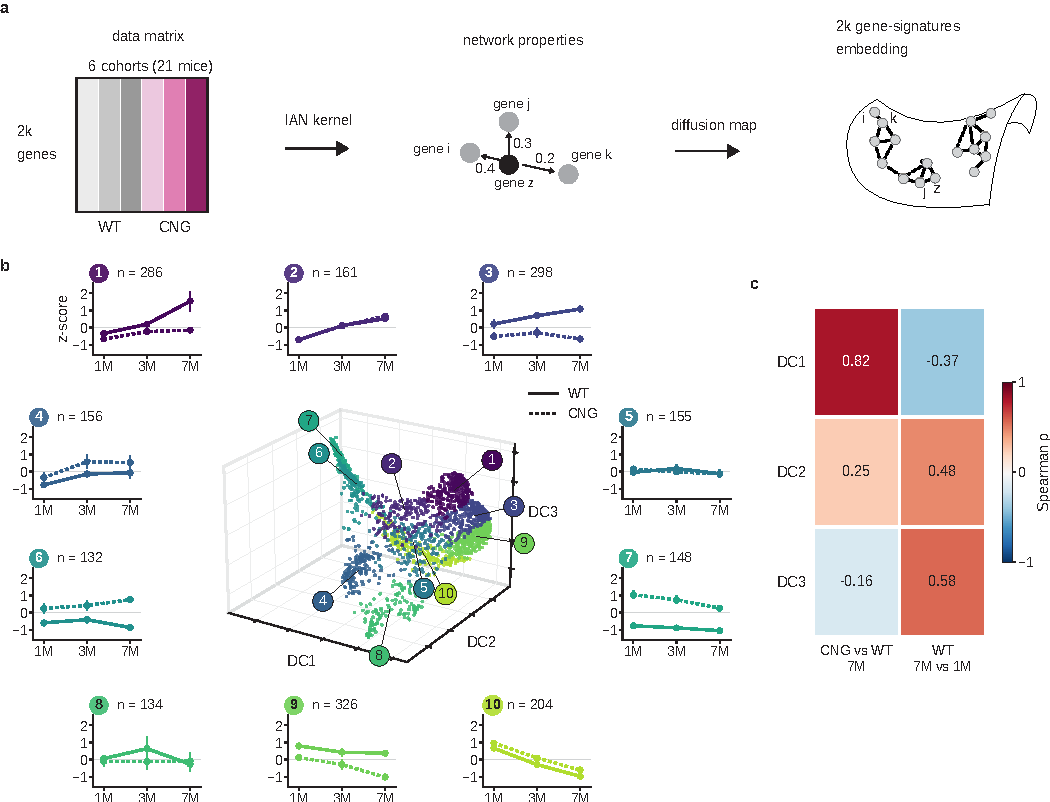
\includegraphics[width=1.0\textwidth]{final-figures/fig2-Kais.pdf}
    \caption{\textbf{Manifold inference reveals the topological landscape of retinal degeneration.} 
    (\textbf{a}) Schematic of the computational workflow: genes and cohorts are organized into a tensor; the IAN kernel is used to identify network properties; diffusion maps are used to organize the network properties into a low dimensional representation. 
    (\textbf{b}) Gene manifold shown for the first three diffusion coordinates (DC) and points colored by local density (Gaussian KDE). 
    (\textbf{c}) Same as \textbf{b} but shown in just two DCs. 
    (\textbf{d}) Spearman correlation analysis linking manifold axes to biological variables, confirming that DC1 and DC2 are highly correlated with disease progression and normal aging, respectively.}
    \label{fig:intro-manifold}
\end{figure}

Applying this approach to transcriptomic data required organizing these data into a matrix of expression levels of 2000 genes by 21 animals, where the animals were organized into 6 cohorts: WT and \cngb retinas harvested at 1, 3, and 7 months of age. Each gene is thus a point whose coordinates are its expression levels across conditions. We used IAN to infer the neighborhood graph over genes, then diffusion maps \citep{Coifman2005-te} to embed that graph in a lower-dimensional space (Figure \ref{fig:intro-manifold}a); we refer to the result as the IAN manifold. The resulting manifold organizes genes according to changes in their expression levels across conditions (Figure \ref{fig:intro-manifold}b,c): each point represents a gene and genes nearby on the manifold exhibit similar changes in expression across conditions. The data are represented in diffusion coordinates (DCs; e.g., DC1 and DC2). These DCs were highly correlated with particular experimental variables. For example, DC1 was highly correlated with changes in gene expression between late stage photoreceptor degeneration (\cngb mice at 7M) compared with age-matched WT mice (Figure \ref{fig:intro-manifold}d). 

The organization of genes on the manifold is made clearer by partitioning it into local neighborhoods and plotting their expression levels across normal aging and degeneration (Figure \ref{fig:neighborhoods}a). For example, neighborhood 1 (dark blue) identifies genes whose expression increases with age but stays relatively flat during degeneration; neighborhood 3 (light green) identifies genes that decrease in both; and neighborhood 10 (dark red) is formed by genes that are low and constant during normal aging but elevated during degeneration.  


\begin{figure}[htbp]
    \centering
    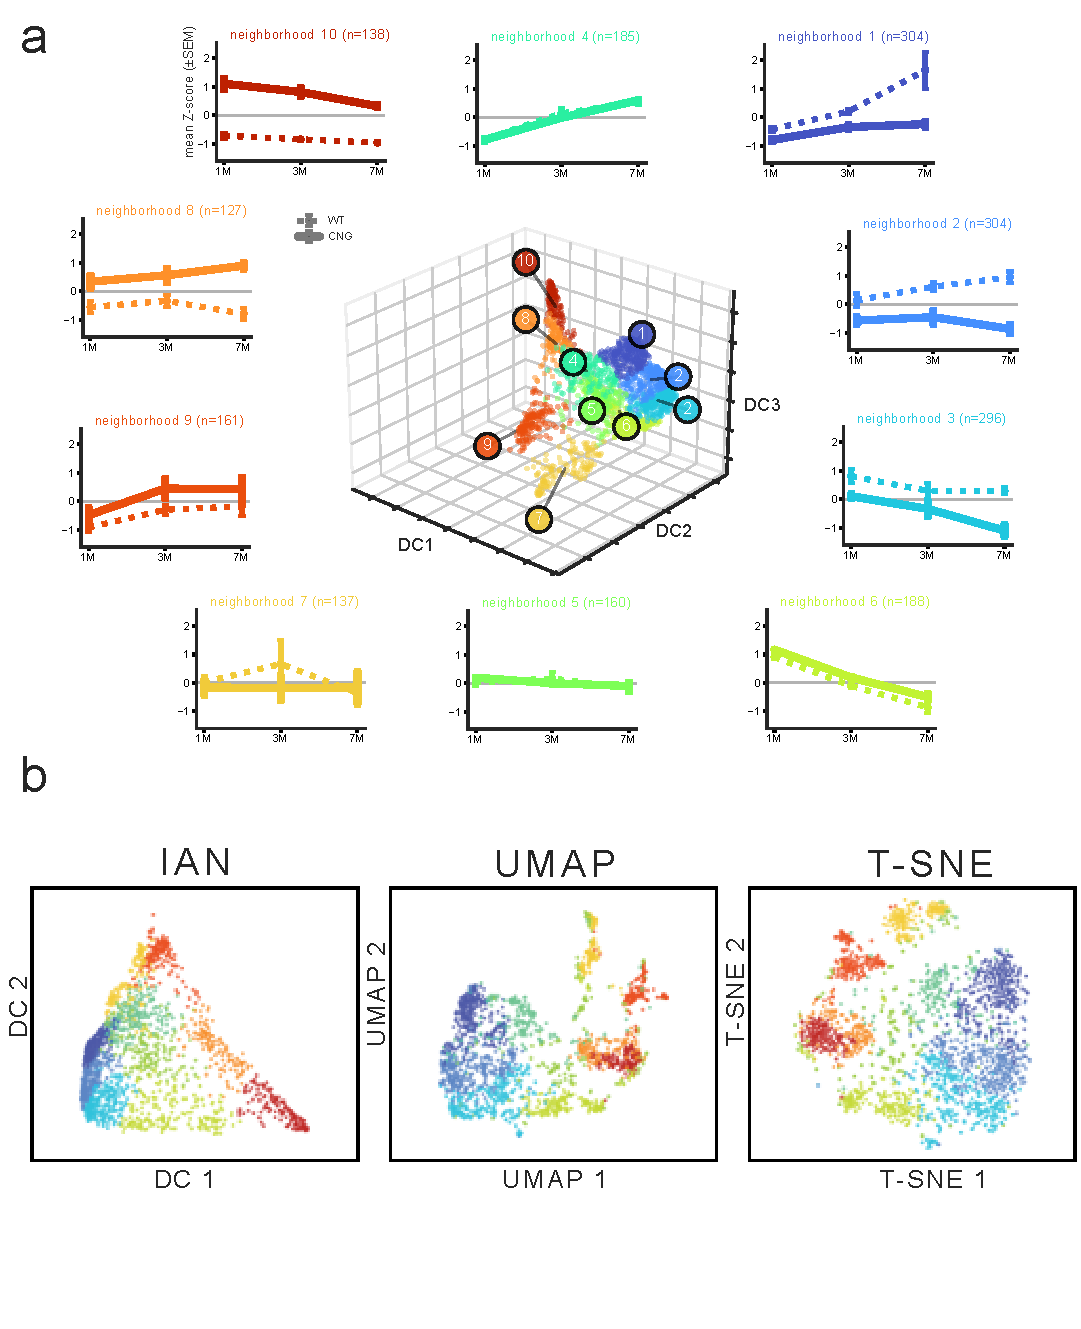
\includegraphics[width=0.7\textwidth]{final-figures/fig3.pdf}
    \caption{\textbf{Spatiotemporal organization of the ON bipolar cell transcriptomic manifold.} 
    (A) Three-dimensional gene manifold partitioned into discrete neighborhoods using automated density peak clustering. 
    (B) Z-scored expression trajectories for divergent manifold neighborhoods in healthy control (WT) and \textit{Cngb1$^{neo/neo}$} (CNG) cohorts.
    (C) Volcano plot of late-stage disease (CNG 7M vs WT 7M) colored by manifold neighborhood. The topological organization of the manifold accurately segregates transcriptomic outcomes, with key remodeling markers (\textit{Stat3}, \textit{Edn2}) and structural transcripts (\textit{Prph}) localizing to specific neighborhoods.}
    \label{fig:neighborhoods}
\end{figure}


\subsection*{Comparison to other common visualizations}

UMAP and t-SNE are the most popular algorithms for visualizing transcriptomic landscapes. Both build a neighborhood graph using a fixed number of neighbors and optimize a layout that preserves local relationships. Importantly, the optimization is stochastic in each case, so repeated runs give different embeddings unless random seeds are fixed. Their objectives target local distance structure, and mesoscale and global relationships in the data are correspondingly less well preserved, which can support false or misleading premises about overall organization of the data. Our pipeline differs in both respects: IAN infers the neighborhood graph without a fixed neighborhood size, and diffusion maps embeds it using eigenvectors of the graph Laplacian, which depend on connectivity throughout the graph rather than on nearest-neighbor relations alone. Diffusion distances therefore reflect relationships at all scales, and the embedding is identical on every run. Thus, we compared the spatial relationships among genes generated by the three approaches.

First, we clustered genes by k-means in the IAN manifold. This resulted in groups of genes whose expression profiles changed similarly across aging and degeneration (Figure XX). We then painted these cluster identities onto the UMAP and t-SNE embeddings. The identities are visibly intermixed in both, whereas they are compact in the IAN manifold, as quantified by the tightness of each cluster (Fig XX). A grouping defined in one embedding will tend to look coherent there, so we reversed the analysis: we clustered genes in the UMAP and t-SNE embeddings and looked at how these gene groups changed across aging and degeneration. Mean expression profiles within these groups were (on average) flat and highly variable across genes within a group, unlike the IAN clusters (Fig XX). Proximity in the IAN manifold therefore corresponded to shared expression dynamics, which is what the analyses below depend on; proximity in the UMAP and t-SNE embeddings did so far more weakly.


\subsection*{Normal aging in early adulthood alters ON bipolar cell gene expression} 

One application of this manifold embedding is to visualize and identify gene expression changes between cohort pairs (e.g., 3M to 7M healthy aging animals) within the larger context of gene expression changes across both aging and degeneration. Thus, using only WT data, we first analyzed cohorts of genes that changed expression levels across the different ages of mice (Figure \ref{fig:aging}). We began with analyzing the largest age gap: 1M to 7M animals. Genes with statistically significant changes in expression between these two ages were identified on the manifold, with point size indicating statistical significance and color indicating magnitude (Figure \ref{fig:aging}A). This analysis showed a substantial number of genes (XX) that displayed statistically significant changes in gene expression over early to mid adulthood. This indicates ON bipolar cell transcriptomes are not particularly stable over adulthood. We also identified the top 10 most up and down regulated genes between the two cohorts (Figure \ref{fig:aging}B). Many of these genes such as XX and XX have been associated previously with aging processes. 

\begin{figure}[htbp]
    \centering
    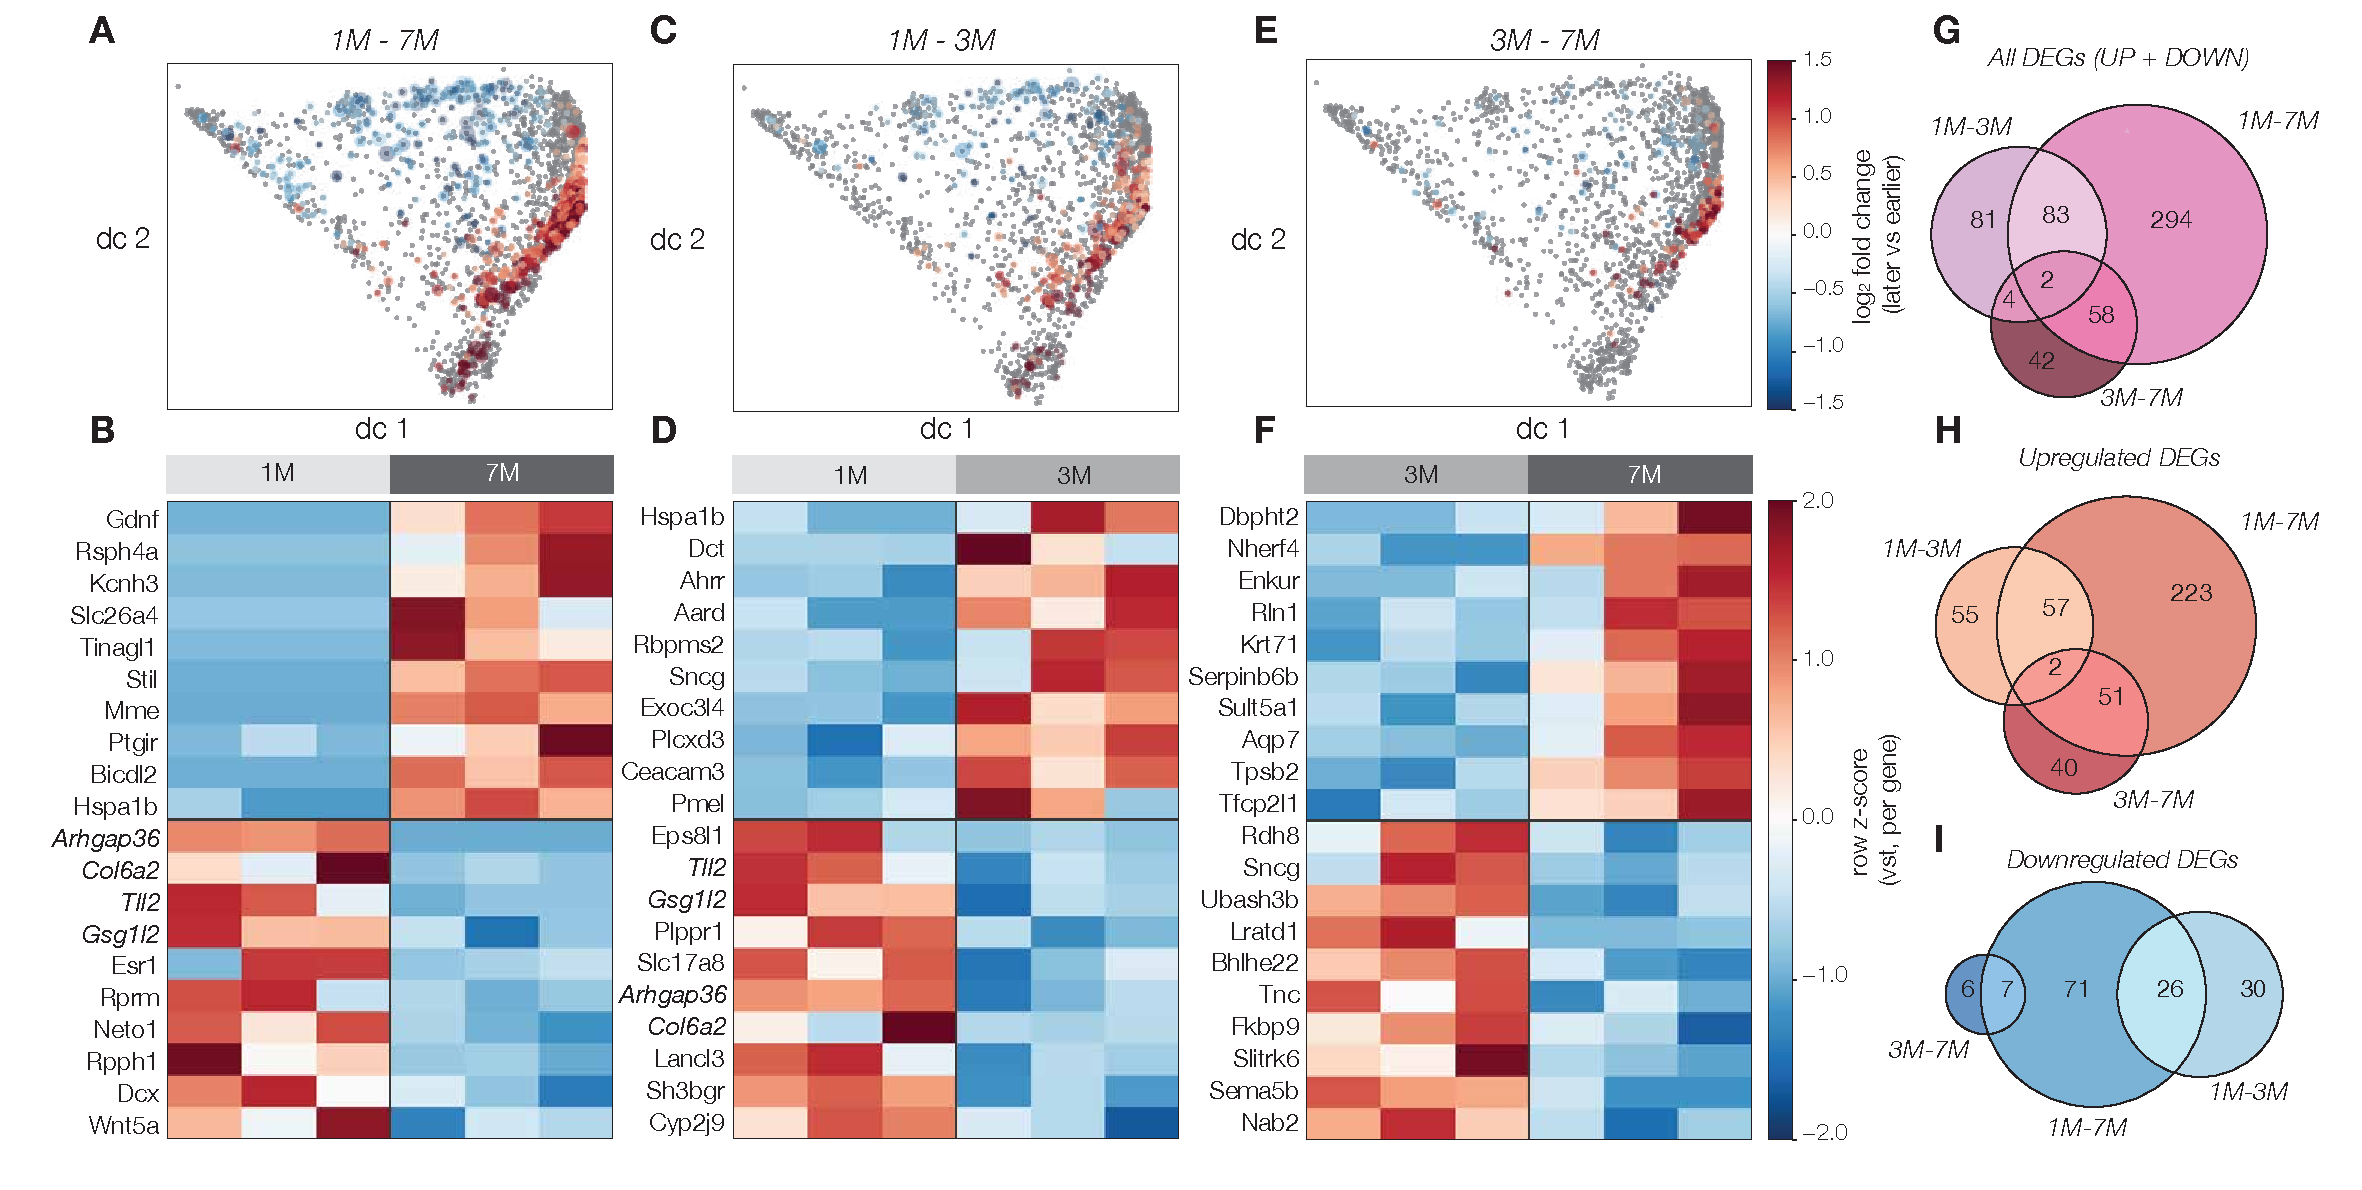
\includegraphics[width=1.0\textwidth]{final-figures/Aging.pdf}
    \caption{ON Bipolar cell transcriptomes change substantially over early to mid-adulthood in normally aging retinas. (\textbf{A.}) Manifold identifying gene changes between 1M and 7M cohorts of WT mice. Point size indicates statistical significance and color indicates magnitude. (\textbf{B.}) Ten most up (top) and down (bottom) regulated genes between 1M and 7M. Each row is a gene, each column show expression level in one animal. (\textbf{C, E}) Same as A, but for 1M to 3M and 3M to 7M, respectively. (\textbf{D, F}) Same as B, but for 1M to 3M and 3M to 7M, respectively. (\textbf{G-H}) Venn diagrams indicating the numbers of shared and distinct genes that are differentially expressed (G), up regulated (H) and down regulated (I) across the three pairwise comparisons of the normal aging cohorts.}
    \label{fig:aging}
\end{figure}

While the 1M time point should be at or very near the close of the developmental window for the retina \textbf{(references)}, it is possible some developmental processes have not completely ended, thereby confusing genes associated with development to genes associated with post-developmental aging. Thus, we also analyzed changes in gene expression between 1M and 3M and between 3M and 7M healthy ON bipolar cells (Figure \ref{fig:aging}C-F). 3M is well past the development of the retina. Some genes did change more substantially between 1M and 3M, such as Ahrr, which negatively regulates cell growth, and Plppr1, involved in synapse formation. However, many genes also changed expression levels substantially between 3M and 7M (Figure \ref{fig:aging}E-F), such as Nher4f, encoding a scaffolding protein,  and Sema5b, related to axon guidance. This indicates that even into adulthood ON bipolar cell expression patterns changes with age in mouse. The genes changing the most across all three pairwise cohort comparisons inhabited highly overlapping neighborhoods on the manifold, with down regulared genes generally along the top edge, and up regulated genes generally along the right edge (Figure \ref{fig:aging}A, C, E). These qualitative patterns will change when we turn our attention to the impact of degeneration on gene expression.

The Venn diagrams summarize the numbers of genes in each cohort comparison and how many genes were shared between cohort comparisons. Several patterns are worth noting. First, the cohort comparison with the largest change in gene expression is the 1-7M. This could be because 1M is catching the tail-end of development, or because this is the largest age gap. Possibly supporting the hypothesis that 1M captures the end of development, changes in gene expression between 1M and 3M were more numerous (170 genes) than between 3M and 7M (106 genes; Figure \ref{fig:aging}G). Interesting, relatively few genes with statistically significant differential expression were shared between the 1-3M and 3-7M comparisons. Second, the sum of differentially expressed genes between 1-3M and 3-7M totals 276 genes, much less than the 435 genes that significantly changed between 1-7M. This suggests we are likely statistically underpowered in identifying all of the significantly changing genes, presumably because the magnitude of the expression level changes is smaller on the shorter compared to longer timescales. Finally, many more genes were upregulated over aging than down regulated for all three pairwise comparisons (Figure \ref{fig:aging}H-I). 

\subsection*{Photoreceptor degeneration leads to extensive changes in ON bipolar cell gene expression} 

We next performed a similar set of analyses, but between animals of matched age with or without retinal degeneration (Figure \ref{fig:degen}). Perhaps the first feature to notice is how differently the manifolds are colored for the control age comparisons (Figure \ref{fig:aging}) versus control compared to \cngb mice (Figure \ref{fig:degen}): the manifolds are the same (generated from all data), but the highlighted neighborhoods are quite different. Genes up regulated between healthy and degenerating retinas were localized in the left corner and left edge of the manifold; genes down regulated were localized along the top right edge. For all three cohort comparisons between healthy and \cngb animals, the neighborhoods on the manifold are relatively conserved, with the 7M comparison (Figure \ref{fig:degen}E) the most expansive neighborhoods of differential gene expression. The genes with the largest differential expression were also more consistent in the degeneration comparisons than in the aging comparisons (genes with bold and italic names in Figure \ref{fig:degen}B, C, F). Specifically 4 up regulated genes, Prhp, Dlx3, A2m and Fgf2, were strongly up regulated at 1, 3 and 7 month time points. No gene was up or down regulated in all three comparisons for the aging comparisons, but a few appeared in two comparisons (italic genes in Figure \ref{fig:aging}B, C, and F). 

The Venn diagrams summarizing the changes between health at degenerating retinas at different ages also demonstrate different patterns of expression compared to the aging comparisons. Significantly up regulated genes (125) outnumbered down regulated genes (25) at 1M. At 3M, the comparison was more balanced (137 up- and 101 down-regulated). At 7M, significantly down regulated genes (290) outnumbered up regulated genes (106). Overall, there was a clear trend for more genes to be more strong differentially expressed with increasing age: 150 genes at 1M, 238 genes at 3M, and 396 genes at 7M. Thus, perhaps unsurprisingly, as degeneration progressed from 30\% rod death (1M) to 70\% (3M) to ~100\% (7M), ON bipolar cell transcriptomes exhibit more numerous differences in gene expression relative to age-matched control animals. 


\begin{figure}[htbp]
    \centering
    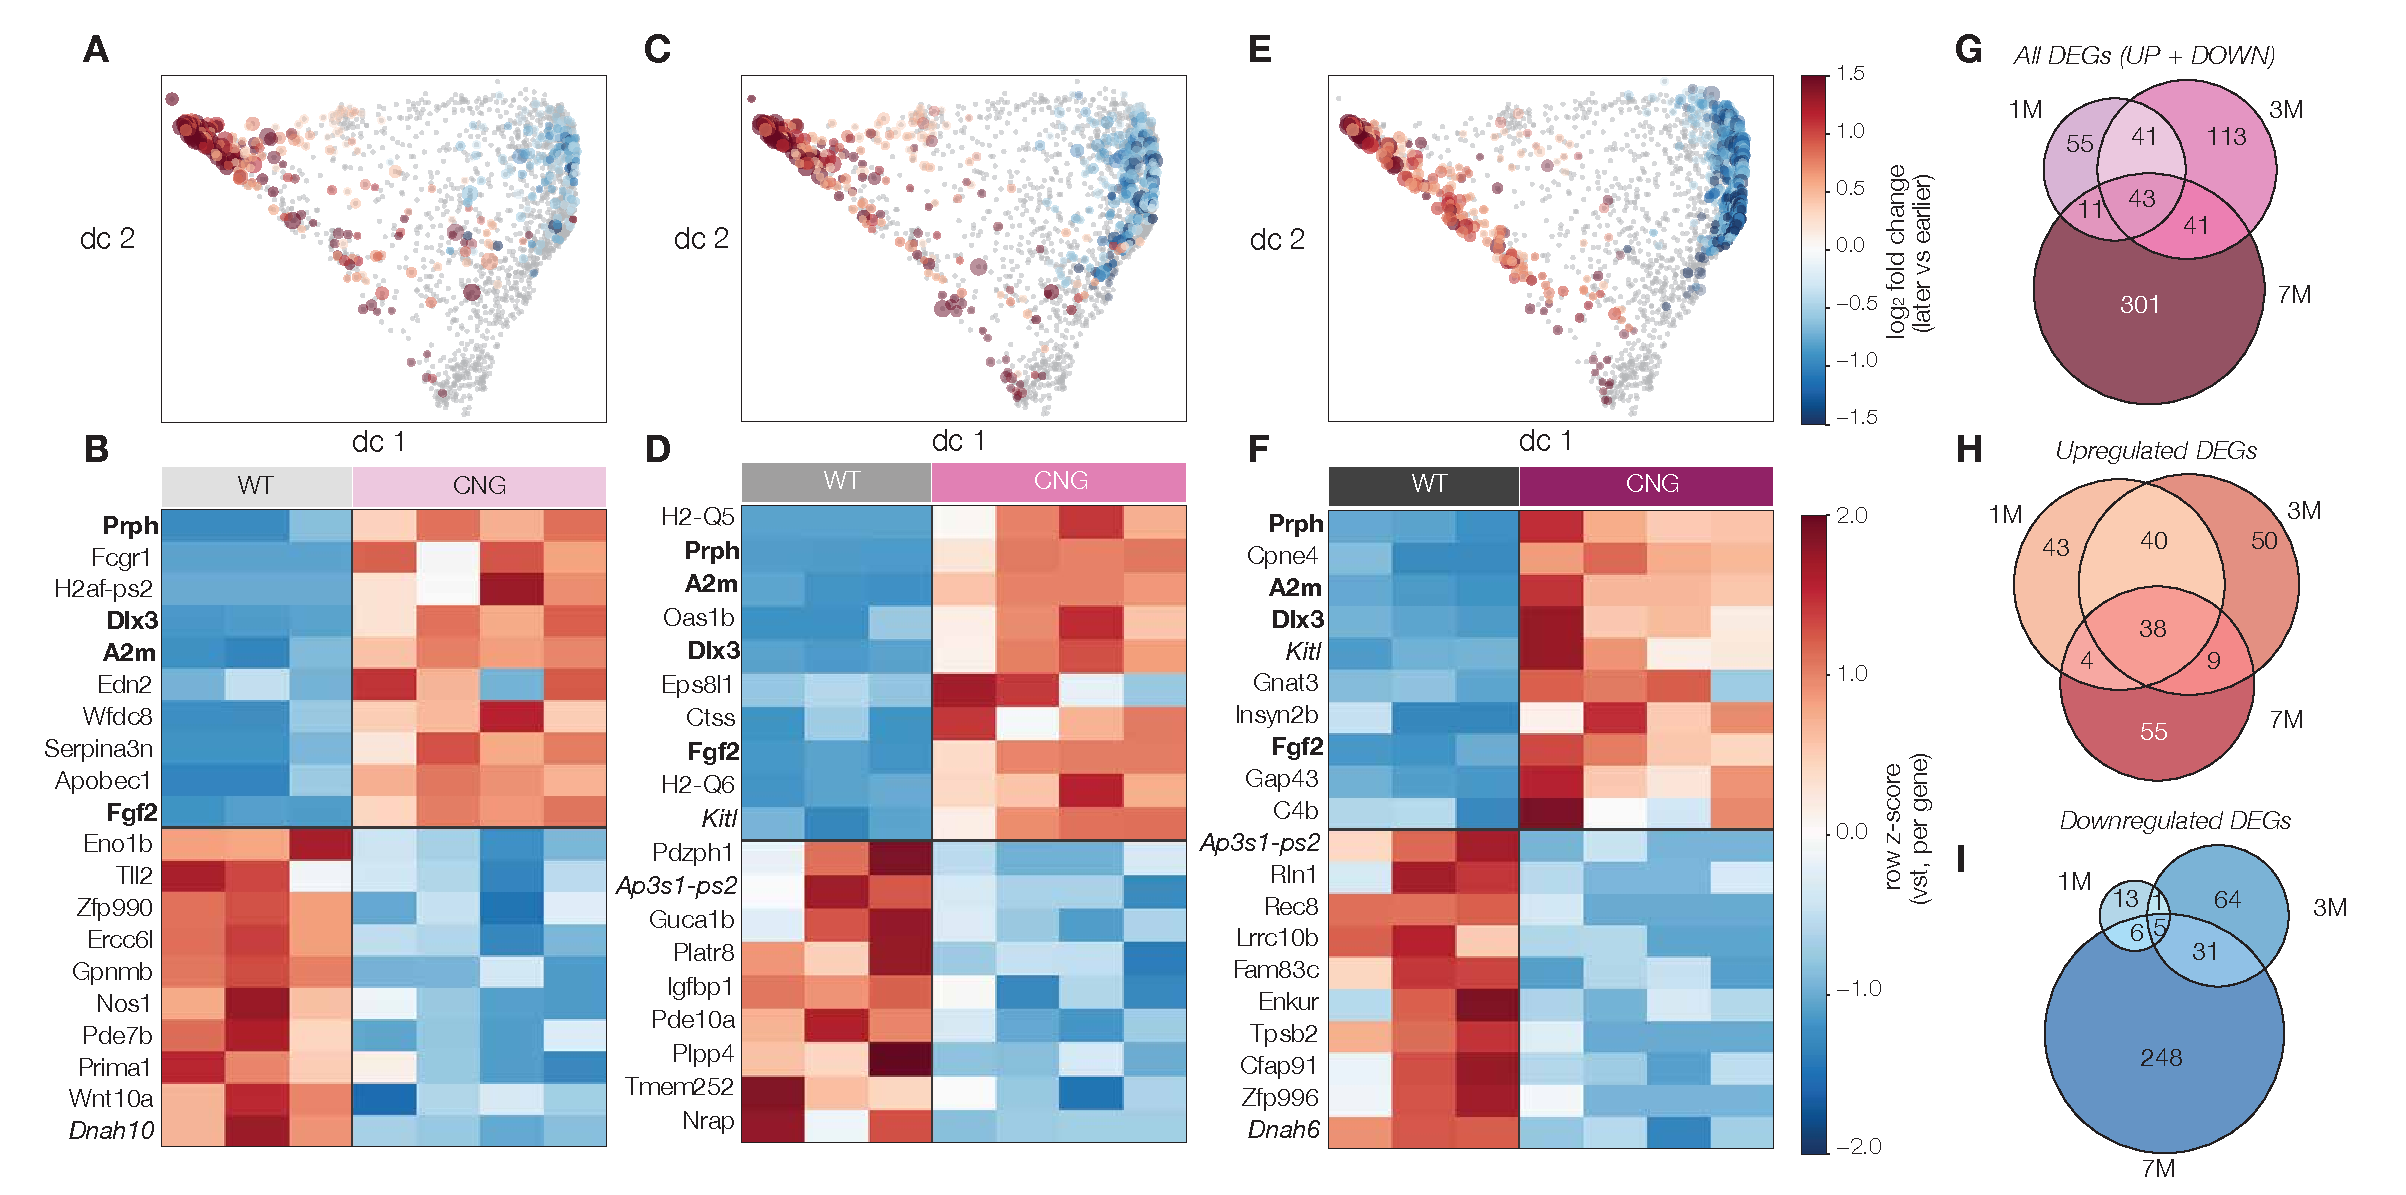
\includegraphics[width=1.0\textwidth]{final-figures/disease.pdf}
    \caption{Photoreceptor degeneration causes expanding changes in bipolar cell transcriptomes. (\textbf{A.}) Manifold identifying gene changes between 1M control and 1M \cngb mice. Point size indicates statistical significance and color indicates magnitude. (\textbf{B.}) Ten most up (top) and down (bottom) regulated genes between 1M control and 1M \cngb mice. Each row is a gene, each column shows expression levels in samples in one animal. (\textbf{C, E}) Same as A, but between 3M control and 3M \cngb and between 7M control and 7M \cngb mice, respectively. (\textbf{D, F}) Same as B, but between 3M control to 3M \cngb and between 7M control to 7M \cngb, respectively. (\textbf{G-H}) Venn diagrams indicating the numbers of shared and distinct genes that are differentially expressed (G), up regulated (H) and down regulated (I) across the three pairwise comparisons between control and \cngb retinas.}
    \label{fig:degen}
\end{figure}


\subsection*{Analysis of disease-specific progress identifies a relatively small number of key genes.}

The previous analysis compared ON bipolar cell gene expression between age-matched control and \cngb mice. While highlighting differences in gene expression between healthy and control animals, it does not necessarily identify or highlight genes that are key in disease progression. Therefore, we made comparisons between \cngb mice at 1-7M, 1-3, and 3-7M (Figure \ref{fig:progression}), similar to the analysis performed for aging (Figure \ref{fig:aging}). Many genes were differentially expressed in the 1M to 7M \cngb comparison (Figure \ref{fig:progression}A-B), however much smaller numbers of genes reached statistically significant differential expression between 1M-3M and 3M-7M \cngb comparisons (Figure \ref{fig:progression}C-F). These differences are striking in the Venn diagrams summarizing these numbers (Figure \ref{fig:progression}G-I). This is likely because the variances in gene expression profiles across animals were significantly more variable in the \cngb compared with control mice (\textbf{INCLUDE SOME VARIANCE ANALYSIS HERE}). 

\begin{figure}[htbp]
    \centering
    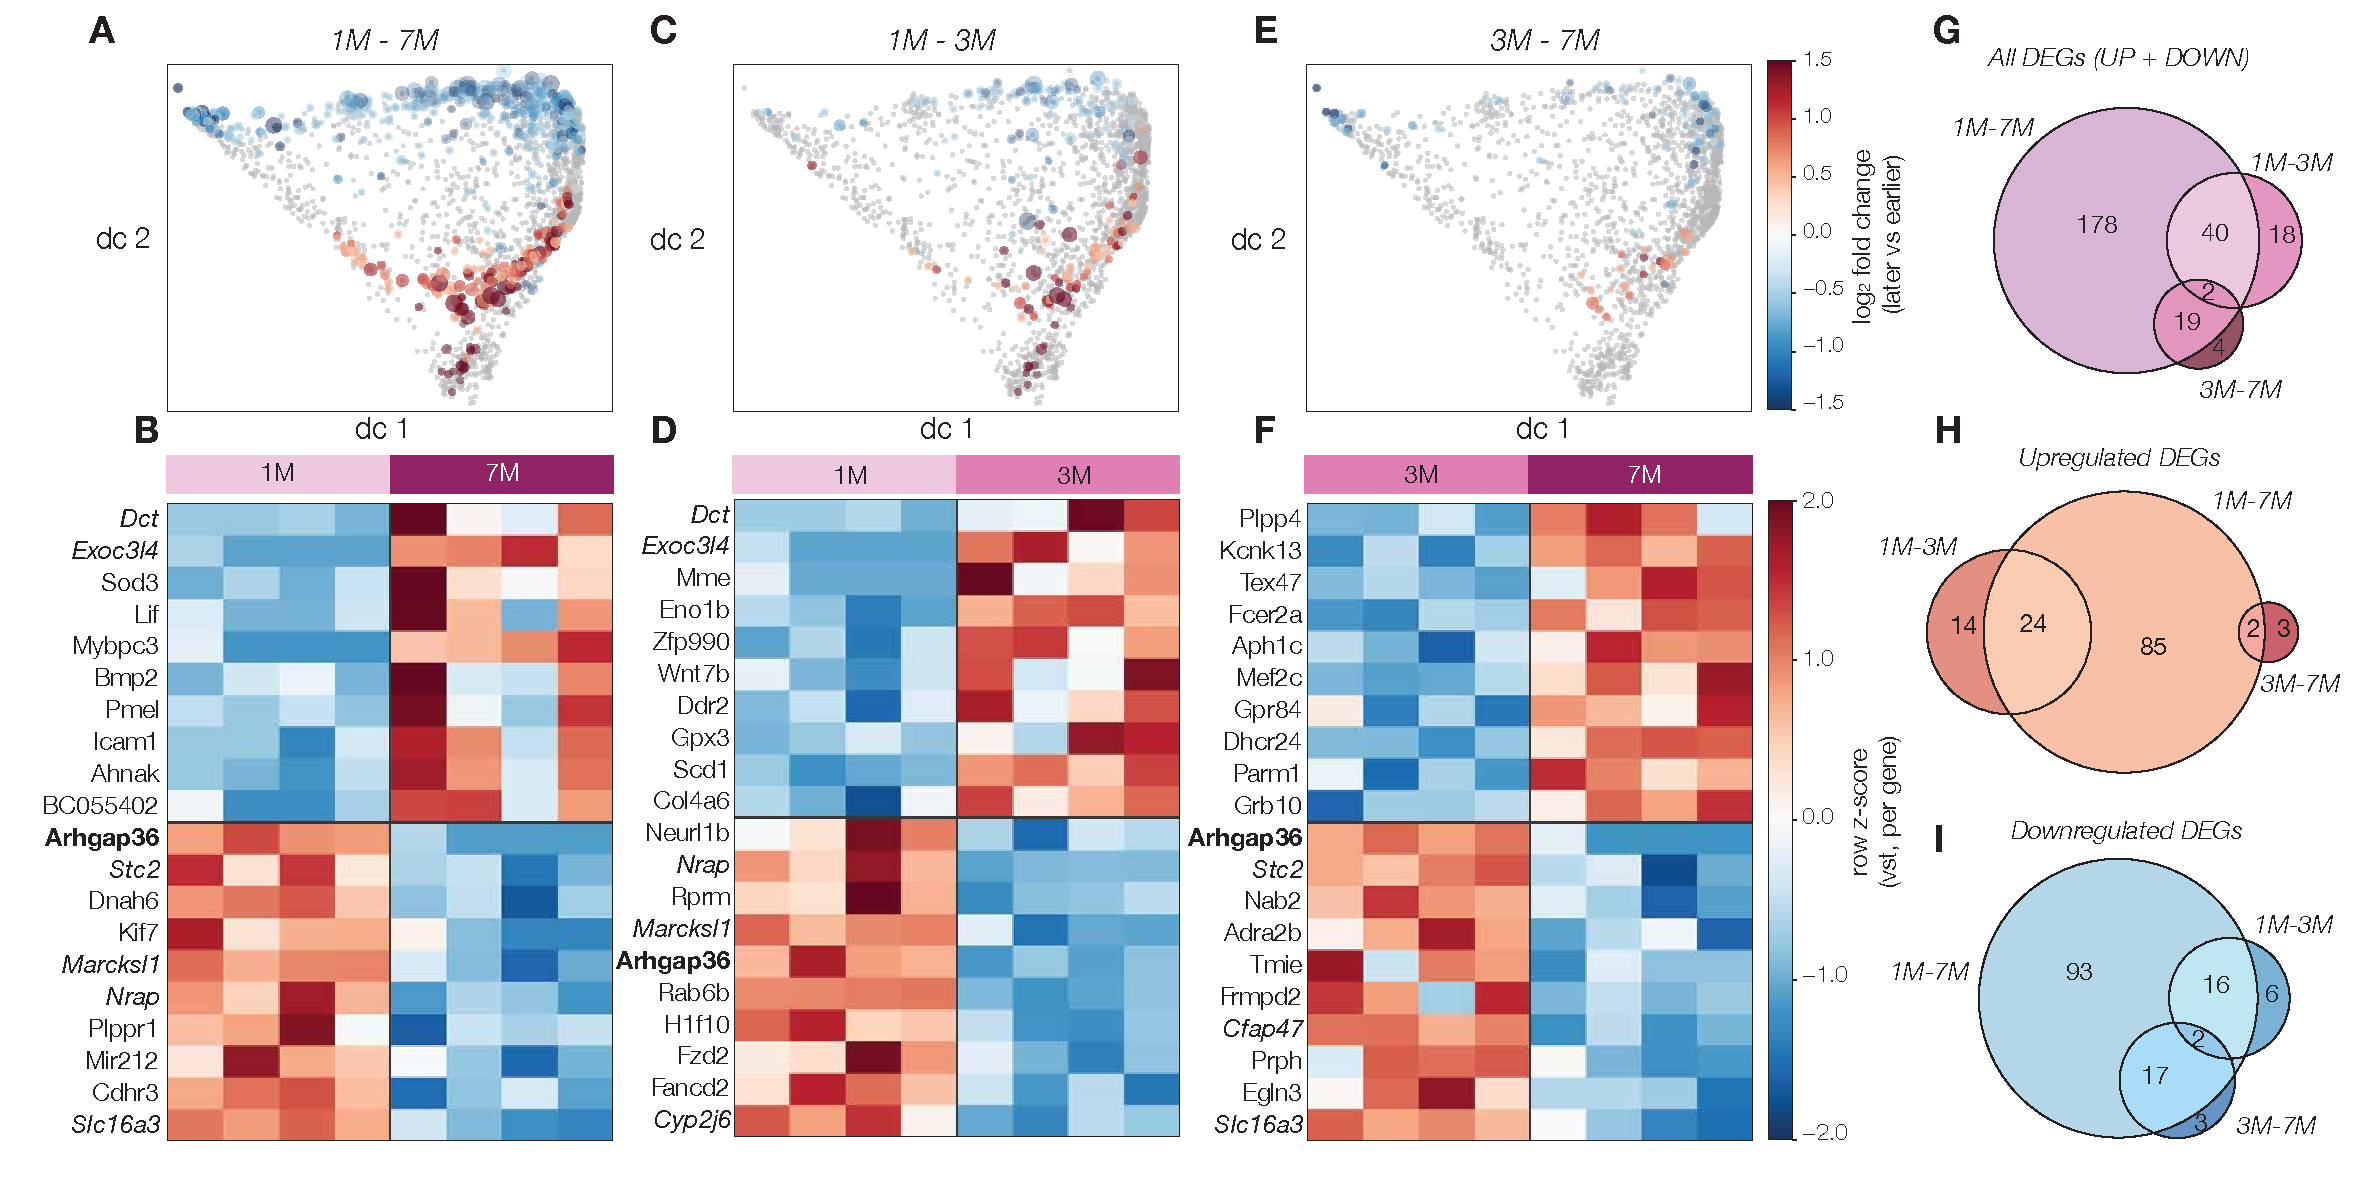
\includegraphics[width=1.0\textwidth]{final-figures/progression.pdf}
    \caption{Gene networks changing with disease progression. (\textbf{A.}) Manifold identifying gene changes between \cngb mice at 1M and 7M. Point size indicates statistical significance and color indicates magnitude. (\textbf{B.}) Ten most up (top) and down (bottom) regulated genes between 1M and 7M \cngb mice. Each row is a gene, each column shows expression levels in samples in one animal. (\textbf{C, E}) Same as A, but between 1M and 3M \cngb and mice between 3M and 7M \cngb mice, respectively. (\textbf{D, F}) Same as B, but between 1M and 3M \cngb mice and between 3M and 7M \cngb mice, respectively. (\textbf{G-H}) Venn diagrams indicating the numbers of shared and distinct genes that are differentially expressed (G), up regulated (H) and down regulated (I) across the three pairwise comparisons \cngb mice at different 1, 3 and 7M.}
    \label{fig:progression}
\end{figure}


Visual inspection of the manifold highlighting gene expression changes for 1M-7M normal aging (Figure \ref{fig:aging}A) with that highlighting expression changes for 1M-7M \cngb progression (Figure \ref{fig:progression}A) reveals overlapping, but shifted gene neighborhoods. Down regulated genes are more tightly grouped along the top edge of the manifold and more cluster in the left corner in the \cngb comparison relative to normal aging. Up regulated genes shift down and extend to the left edge of the manifold in the \cngb comparison relative to normal aging. The fact that these neighborhoods are overlapping, but they are not the same makes intuitive sense: the \cngb disease progression includes the aging process along with the degenerative process. Thus, we analyzed the overlap of genes identified as differentially expressed across aging groups that were also differentially expressed in \cngb progression (Figure XX). A Venn diagram of differentially expressed genes between 1M-7M control mice and 1M-7M \cngb mice revealed substantial overlap (Figure XX). 

NEED A NEW FIGURE THAT SHOWS UP AND DOWN REGULATION OF GENES ON THE MANIFOLD THAT ARE UNIQUE TO DEGENERATION PROGRESSION. 





The analysis above (Figure XX) compares healthy gene expression to that found in degenerating retinas at particular time points. However, it does not highlight expression level changes over the course of disease that are distinct from those associated with normal aging. To isolate the gene networks that were changed by degeneration by distinct from normal aging process, we identified genes that exhibited statistically significant changes in their expression levels between 1 and 7M \cngb mice, but that either did not change expression between 1 and 7M control mice or changed in the opposite direction (e.g., were down-regulated instead of up-regulated). This isolated a distinct cohort of genes that changed their expression between 1 and 7, 1 and 3, and 3 and 7M in the \cngb mice (Figure XX). GO analyses indicated that these genes were associated with XX, XX and XX biological processes, with an increase in XX between 3 and 7M in the \cngb mice.




%\subsection*{Distinct ON bipolar cell gene networks engaged at different stages of degeneration}

%\textbf{Previous studies of \cngb mice suggest that distinct gene networks may be activated as degeneration progresses \citep{Scalabrino2023-dk}. To examine the expression levels changes across degeneration, we next compared age-matched health mice (\cngbwt) with \cngb mice at 1, 3, and 7M (Figure XX). This comparison revealed distinct gene networks engaged at these different timepoint. For example, at 1M, a GO analysis indicated genes primarily involved in XXX, while at 7M, a GO analysis indicated genes primarily involved in XXX. There was also very little overlap in the genes with the largest changes in expression levels between the different time points.} 


% I'M NOT SURE WHAT WORK ANY OF THE TEXT BELOW IS DOING FOR US, BUT KEEPING IT IN CASE THERE ARE SOME GEMS IN THERE.

\subsection*{Pairwise cohort comparisons in a global context}

The geometry and topology of the manifold summarize the expression profiles of genes across conditions. Thus, we can use the manifold to visualize how particular groups of genes change their expression profiles between particular states, while preserving these genes in a greater context. This is not possible in a volcano plot (Fig XX), which simply compares pairwise changes. To illustrate this, we colored the points (genes) on the manifold according to various criteria such as: (1) normal aging (Fig XX), early degeneration (Fig XX), late degeneration (Fig XX), early-to-late degeneration (Fig XX) and degeneration-specific genes (Fig XX). This approach allows one to visualize how ubiquitous it is for genes to change between two conditions and to visualize the relationship of these genes to others that change under other conditions (e.g., normal aging versus disease-specific changes). Interestingly, some conditions are primarily associated with upregulation of particular sets of genes (e.g., early degeneration (Fig XX)), while other processes engage both up and down regulation of gene networks.   

Categories of aging genes varied. We found upregulation at 1M of genes known to be involved in neuron development, with decreasing expression as the animals age (e.g. Arhgap36, which regulates sonic hedgehog signaling during postmitotic neuron specialization). We also found increasing expression of homeostatic regulators (e.g. Mme, peptide regulation,  and Hfe, iron regulation) as animals age. 

Notable disease specific differential gene regulation includes upregulation of potentially neuroprotective genes Gap43, Kitl, and Fgf2, which may contribute to ON bipolar cell survival. Interestingly, Gnat3, which encodes the G-protein subunit alpha-gustducin, is upregulated specifically in late disease only. While the role of alpha-gustducin in ON bipolar cells has not been defined, alpha-gustducin is a strong marker of type 7 ON bipolar cells and weak marker of rod bipolar cells.  Finally, Mir670hg is downregulated during disease, particularly at 7M. This gene produces microRNA related to retinal damage response. 
\subsection*{Coordinated expression changes in genes associated with synaptic signaling and immune activation}

Through spatial colocalization on the manifold, we identified specific gene sets that exhibited concerted changes (Figure XX). As mentioned, we identified genes associated with 
For instance, the synaptic signaling gene set displayed an upregulation across ages in healthy controls, contrasting with an overall underexpression in \cngb mice. The heatmaps below the manifold image highlight several of these genes, showcasing their expression levels (Figure 3B). The selection of these genes was based on their positions on the manifold, allowing us to discern major changes within this set of genes.


Notably, an additional gene set exhibiting concerted changes was immune response genes (Figure 3C-F). In instances of degeneration, these genes were upregulated, mirroring the histological appearance of retinitis pigmentosa pathology observed. This alignment reinforces the manifold's ability to not only represent complex gene expression changes but also to link these changes to observable anatomical and histological variations. 

%\subsection*{Identifying individual gene expression changes in degeneration and aging}

%A useful feature of the \cngb mice is that it allows for the genetic rescue of Cngb1 expression by the administration of tamoxifen {references}. In previous work, we found there was a significant difference in functional recovery between Cngb1neo/neo animals treated early versus those treated later. Interestingly, while early treatment facilitated full recovery of visual information transmission through the retinal circuitry, late treatment did not yield the same positive outcomes. These results indicate the retinal circuitry is not recovering at this later time point, though it is unclear which, if any, underlying molecular mechanisms govern these divergent responses. By scrutinizing transcriptomic alterations, we aimed to identify the molecular mediators that contributed to the more optimal signal propagation. 

%Notably, the Cngb1neo/neo mouse line enables a model of gene replacement therapy without variables associated with viral therapy. Treatment was delivered at two distinct ages corresponding to time points utilized in Scalabrino \& Thapa et al., 2023: 1 month (1M), or early treatment when ~25% of rods have died, and 3 months (3M), or late treatment when ~70% of rods have died.

%To analyze the data generated from this experiment, we reconstructed the manifold using data solely from untreated animals. This manifold served as a reference point to contextualize gene expression changes in response to treatment. Additionally, we expanded the gene list to encompass genes affected by treatment, ensuring a thorough assessment of transcriptomic alterations. To discern the impact of treatment on gene expression patterns, we calculated z-scores to highlight the fractional change observed for each gene between older untreated animals (7 months) and older treated animals (5 months). This updated methodology offers a nuanced understanding of how treatment influences the transcriptomic landscape of bipolar cells amidst degeneration. 

%In our analysis, a prominent feature observed in the early treatment data was the emergence of a large arm distinct from the late treatment group (Figure 5B, 5C). This conspicuous arm, notably absent in the late treatment cohort, delineates a substantial portion of genes that undergo significant changes in expression as a result of early intervention. Specifically, a notable trend observed was the transition of numerous genes from upregulated to downregulated states following early treatment, a phenomenon not observed in the late treatment group. This shift underscores the impact of early intervention in mitigating the transcriptional dysregulation associated with degeneration.

%Moreover, gene ontology analysis revealed that the functional pathways affected by treatment intersected with those identified in our above work. Particularly noteworthy was the downregulation of genes associated with stress response and developmental processes following early treatment (Figure 5D). These findings suggest a potential role for early intervention in modulating key biological pathways implicated in retinal degeneration. The observed downregulation of stress response genes indicates a reduction in cellular stress levels, while the suppression of developmental genes may reflect a stabilization of cellular differentiation processes. Overall, these insights shed light on the multifaceted effects of treatment on the transcriptomic landscape of bipolar cells, offering valuable clues for the development of targeted therapeutic strategies for retinal degenerative disorders.

Two gene sets that exhibited non-coordinated changes, yet displayed alterations, are synaptogenesis genes and developmental genes. The choice to investigate these genes stemmed from their significance in previous studies focusing on degeneration in the visual system, particularly in retinal ganglion cells (RGCs) and primary visual cortex (V1). The rationale behind this exploration lies in the fact that both synaptogenesis and developmental processes entail the formation of synapses, suggesting a potential overlap in the underlying mechanisms during degeneration. Notably, these genes demonstrated a dispersed distribution across the entire manifold, emphasizing the absence of a singular expression trajectory. However, leveraging the manifold allowed us to identify prominent differences in expression patterns for these genes by locating those positioned towards the perimeter of the manifold (Figure 4A-B). An illustrative example is Vsx2, a crucial transcription factor in bipolar cells responsible for their developmental processes, which was downregulated as a consequence of degeneration.




%\begin{figure}[htbp]
%    \centering
%    \includegraphics[width=0.6\textwidth]%{figures/Fig4B_Immune_Activation.pdf}
%    \caption{Aging versus degeneration.}
%    \label{fig:aging-v-degen}
%\end{figure}

%\begin{figure}[htbp]
%    \centering
%    \includegraphics[width=0.7\textwidth]
%{figures/Fig4C_Synaptic_Signaling.pdf}
%    \caption{Aging versus degeneration.}
%    \label{fig:aging-v-degen}
%\end{figure}




\subsection*{Discussion}



\section*{Methods}

\subsection*{Manifold Analysis}

\subsection*{Animal Model}
All animal procedures were approved by Duke University's Institutional Animal Care and Use Committee in accordance with protocol A084-21-04 and aligned with guidelines from the Association for Research in Vision and Ophthalmology. All experiments followed ARRIVE guidelines. \cngb mice (sub-strain C57Bl$/$6J) were bred with Grm6-GFP mice (gift from Shannon Boye, University of Florida) to produce mice with GFP+ ON BCs. Mice were housed in controlled conditions and provided standard chow ad libitum. Both female () and male () mice were utilized. Wild-type (\textit{Cngb1$^{+/neo}$} and \textit{Cngb1$^{+/+}$}) \cngb controls consisted of littermates. Genotyping was conducted by Transnetyx using specific primers. 

\subsection*{Histology and Confocal Microscopy}
Histological procedures were carried out on tissue samples from animals involved in other experiments, following established protocols. Briefly, enucleated eyes were fixed with 4% paraformaldehyde, dissected to remove cornea and lens, eye cups submerged in 30% sucrose, cryopreserved with Optimal Cutting Temperature media, and cryosectioned at 12um. Immunostaining was performed using primary and secondary antibodies, and slides were mounted with DAPI-containing mounting media. Imaging was performed using a Nikon AR1 confocal microscope with ×20 air and ×60 oil objectives and a motorized stage. Images were processed using FIJI. 

\subsection*{Flow Cytometry, RNA Extraction, and Sequencing}
Retinal dissociations were performed using Worthington Papain Kits, as previously described. Briefly, mice were ssacrificed by CO2 inhalation followed by cervical disslocation. Retinas were harvested by placing curved forceps under the eye, slicing the cornea with a razor blade, then pulling up with the forceps. Retina was then isolated from the lens and RPE and submerged into papain solution. Retinas from both eyes were aggregated, but biological replicates were not pooled. 
FACS Sorting: Sorted into lysis buffer
RNA extraction was performed using Qiagen RNeasy Mini Prep Kits (product \#) using manufacturer instructions. 
RNA sequencing
The initial data set contained approximately 55,000 genes. In order to enhance downstream statistical analysis, genes were filtered. First we removed genes that were expressed at very low levels or in 3 or fewer samples. This removed a huge portion of genes, leaving about 25,000. Genes were then annotated for their gene ID using the mygene and pybiomart Python libraries to map the Ensembl IDs to their corresponding gene symbols. Further filtering was done with poorly annotated genes (e.g., symbols with prefixes like ``Gm-'', ``Rik-'', ``AC-'', ``AL-'', or ``LOC-'') in order to ensure biologically relevant interpretations. Finally, this analysis focuses on genes from ON-Bipolar cells. Even with FACS sorting, there is a possibility of contamination from other cell types. To correct for this, a list of known genetic markers from other cell types were created by finding the most highly variable genes in the resulting diffusion map. After these initial filtering steps, about 14,000 genes remained.

Raw reads from RNA-sequencing are not comparable without normalization of the gene counts. This is due to the inherent bias in RNA-sequencing in which longer genes will be read more than shorter gene transcripts, making them appear to be more highly expressed, as well as differences in the total number of reads between samples, which can be highly variable. In order to correct for this, we normalized the raw counts using Transcripts per million (TPM), which takes each genes raw count, divides it by the length of the gene in kilobases to correct for gene length, then scales each sample so that all reads add up to 1 million for each sample, ensuring they can be compared to each other. Further normalization was done by applying a log1p transformation. Log1p is calculated by adding 1 to each TPM count before applying a logarithmic transformation, accounting for values of 0, and reducing the range of expression values to a more normal distribution. 

In order to create the genomic manifold, mean expression for each gene was calculated within each of the 12 cohorts. Variance was calculated for each gene among these 12 cohorts, and the top 2000 highly varying genes were selected for the final expression matrix of 2000 genes $\times$ 12 cohorts. Z-score transformation was applied to this expression matrix, scaling all genes to a mean expression value of 0. This final 2000 gene by 12 cohort expression matrix was used as the input to the IAN algorithm, which constructs a similarity graph between the genes, resulting in a 2000$\times$2000 weighted adjacency matrix. This analysis used the 'correlation' parameter, calculating distance between two genes as 1 - (Pearson correlation coefficient). This adjacency matrix was used as the input for a diffusion map, which uses non linear dimensionality reduction to find the 8 most important axes of variation, or diffusion components.

In order to analyze the multi factorial experimental conditions, a unified model was created using the DESeq2 library in Python. We did this by fitting the GLM model to all 42 samples, incorporating the experimental factors from the metadata (genotype, age, and treatment timing). This allows us to estimate the contribution of each experimental factor on gene expression levels while controlling for the others. It also creates normalized expression counts across all samples which can be compared to each other. By creating this unified model, we could then create contrasts to compare different experimental conditions and test our biological questions.

\begin{figure}[htbp]
    \centering
    % This figure has three panels (A, B, C) using the 'subcaption' package.
    \begin{subfigure}{0.32\textwidth}
        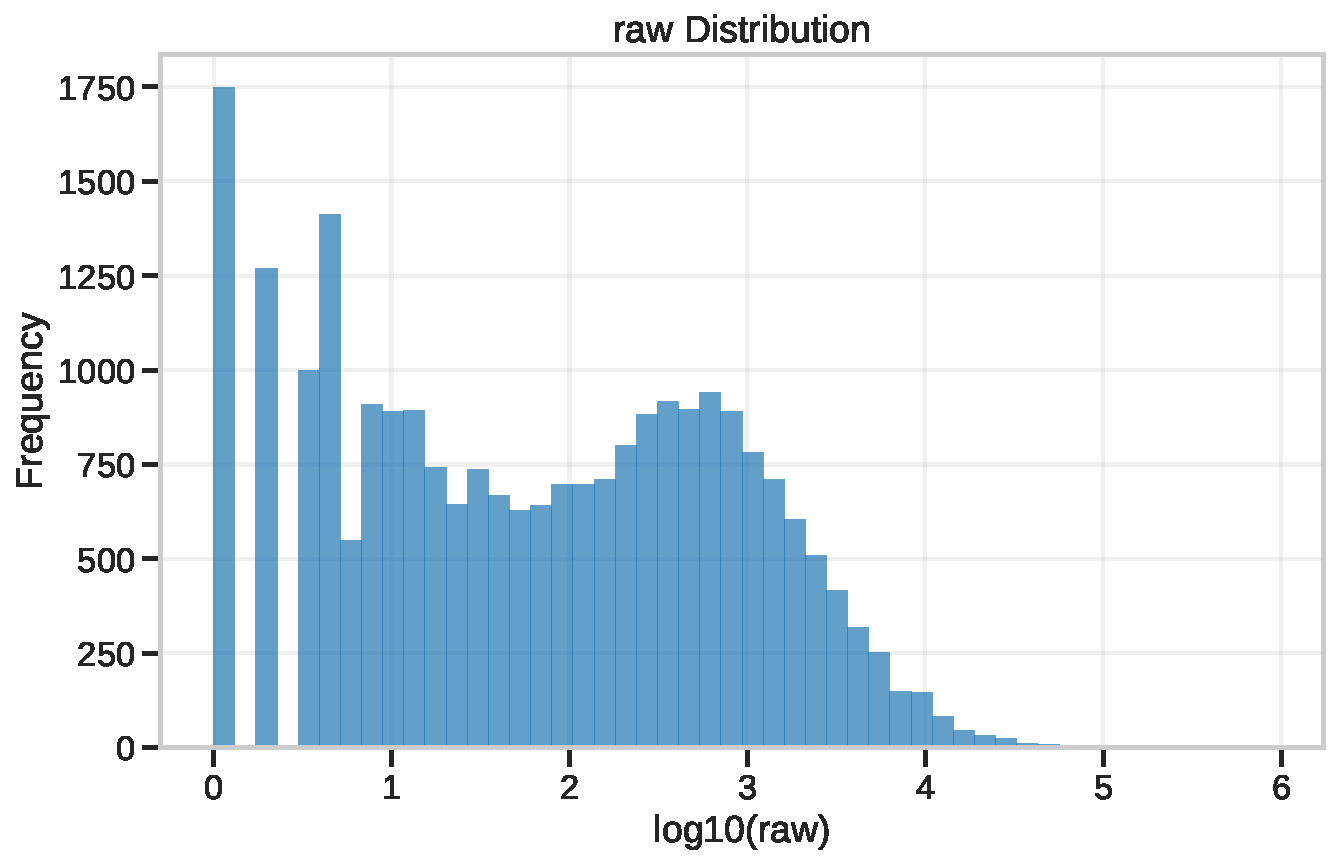
\includegraphics[width=\linewidth]{figures/raw_distribution.pdf}
        \caption{Raw Counts}
        \label{fig:raw_dist}
    \end{subfigure}
    \hfill % Adds space between the subfigures
    \begin{subfigure}{0.32\textwidth}
        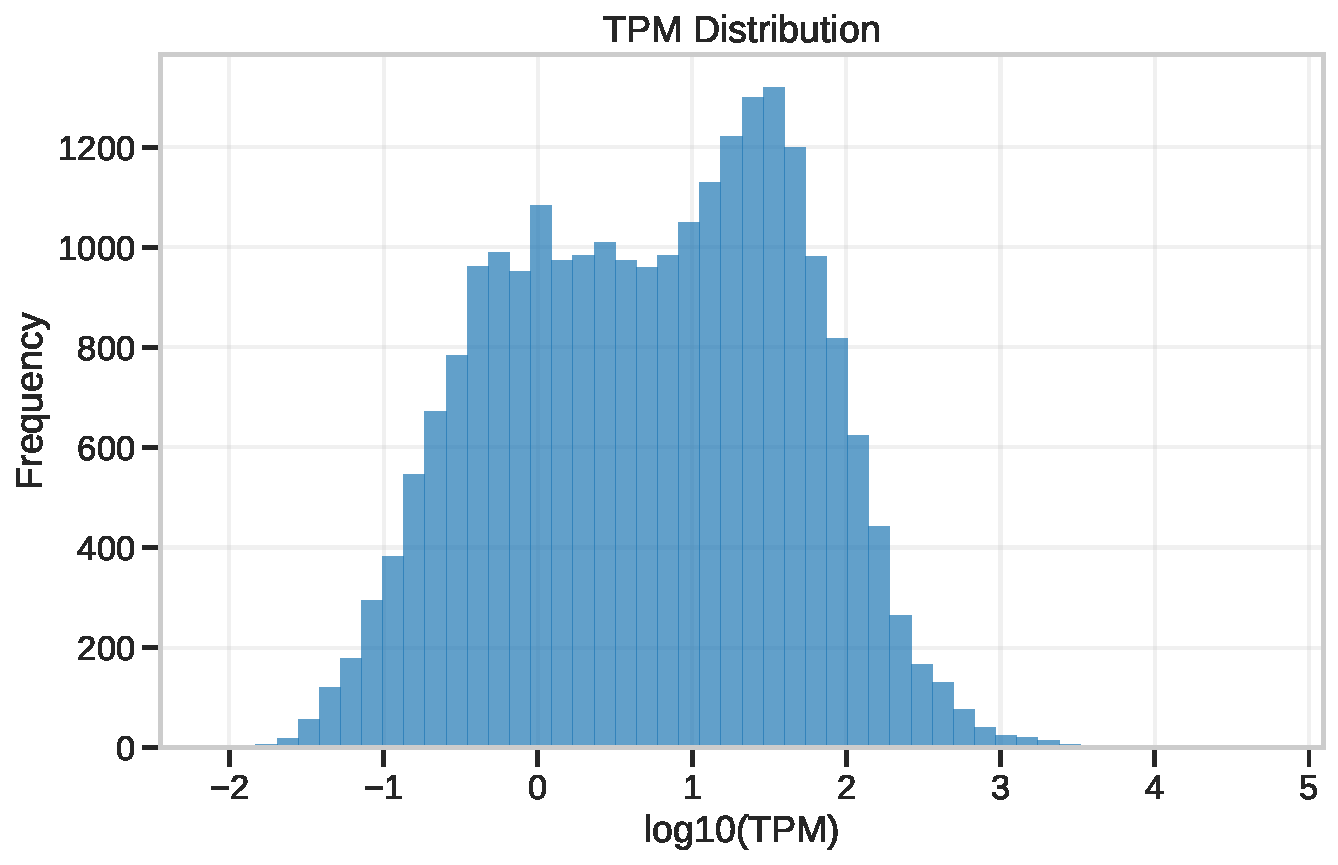
\includegraphics[width=\linewidth]{figures/TPM_distribution.pdf}
        \caption{TPM Normalized}
        \label{fig:tpm_dist}
    \end{subfigure}
    \hfill
    \begin{subfigure}{0.32\textwidth}
        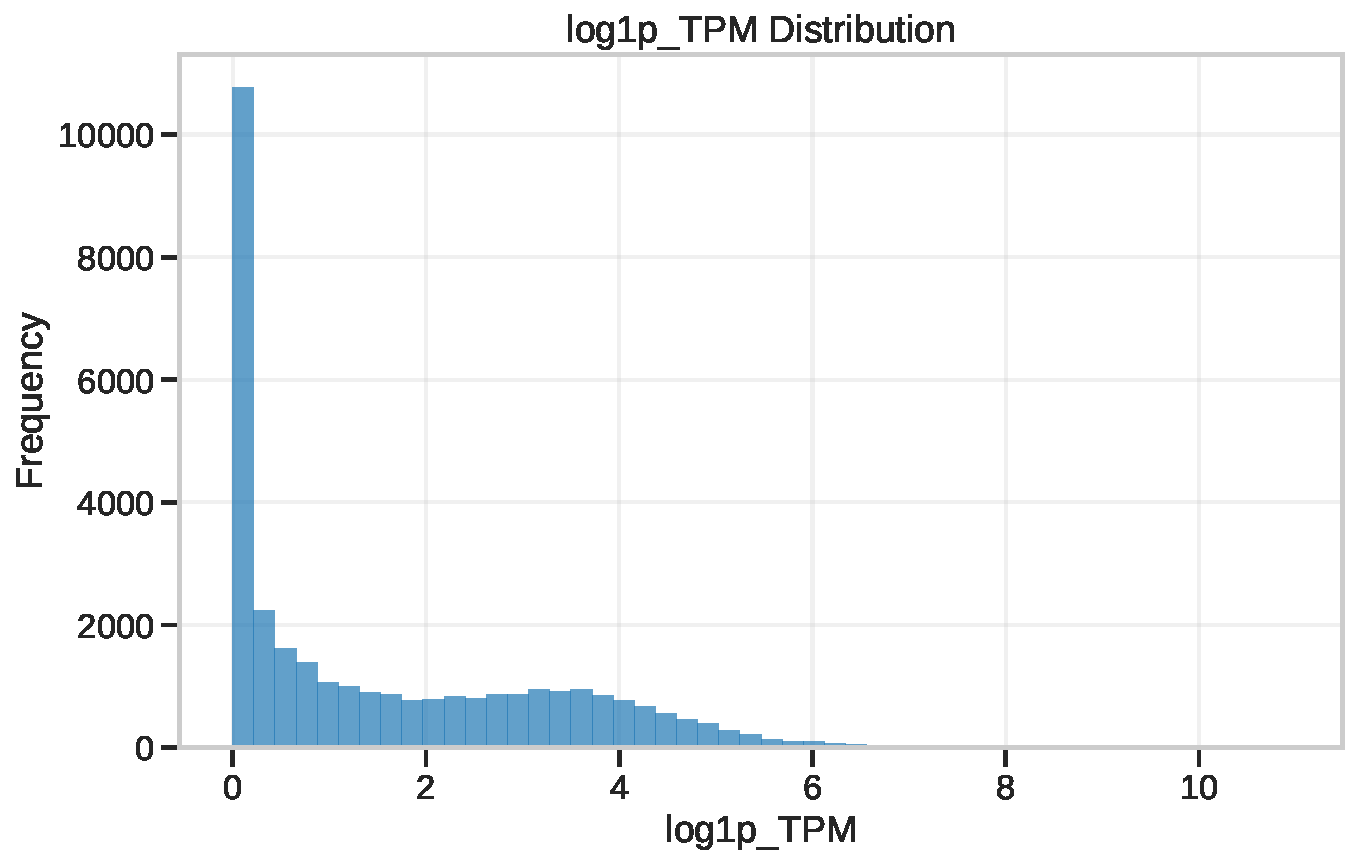
\includegraphics[width=\linewidth]{figures/log1p_TPM_distribution.pdf}
        \caption{Log-Transformed TPM}
        \label{fig:log_dist}
    \end{subfigure}
    \caption{Distribution of gene expression values at key stages of data normalization.}
    \label{fig:normalization}
\end{figure}

\begin{figure}[htbp]
    \centering
    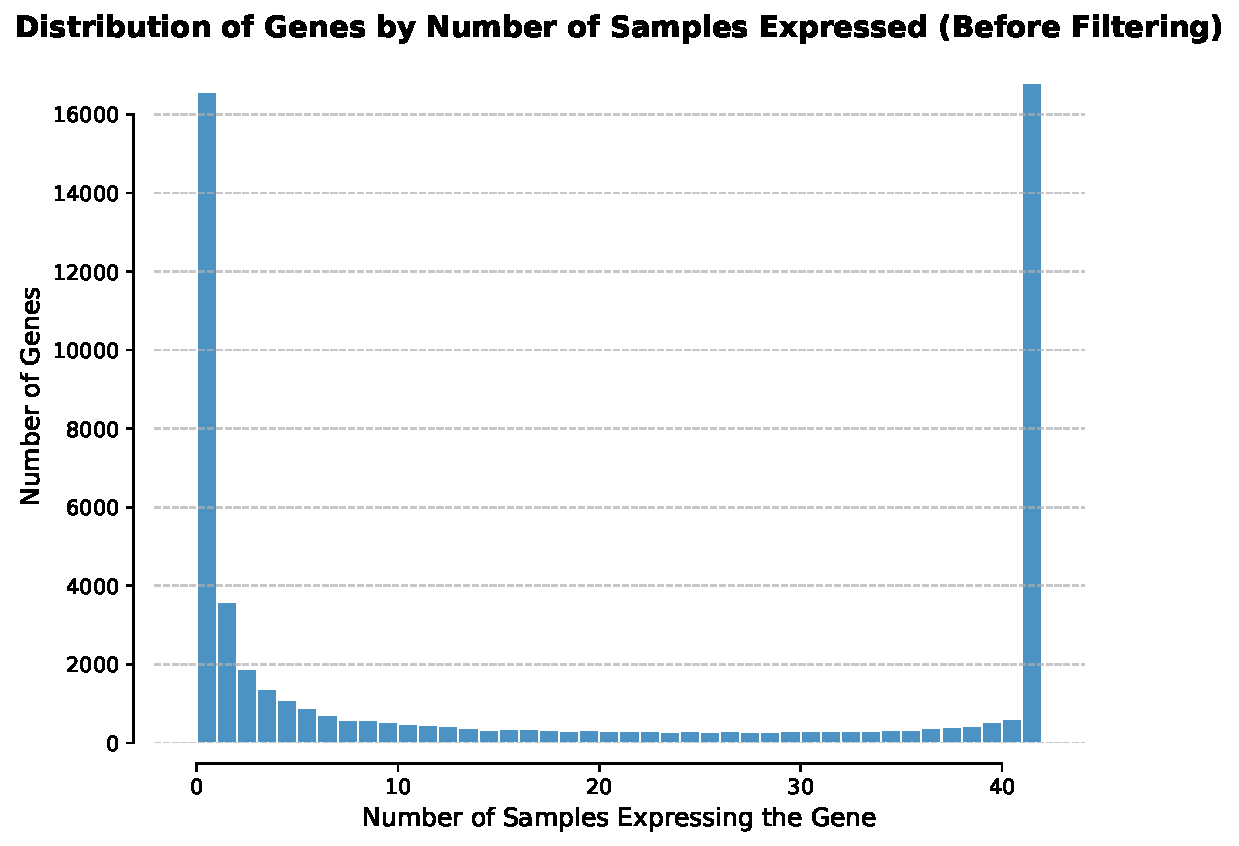
\includegraphics[width=0.7\textwidth]{figures/genes_per_sample_before_filtering_histogram.pdf}
    \caption{Distribution of genes by the number of samples they are expressed in, prior to filtering. This histogram shows that a large number of genes are expressed in very few or nearly all samples.}
    \label{fig:gene_filtering}
\end{figure}


\begin{figure}[htbp]
    \centering
    \begin{subfigure}{0.49\textwidth}
        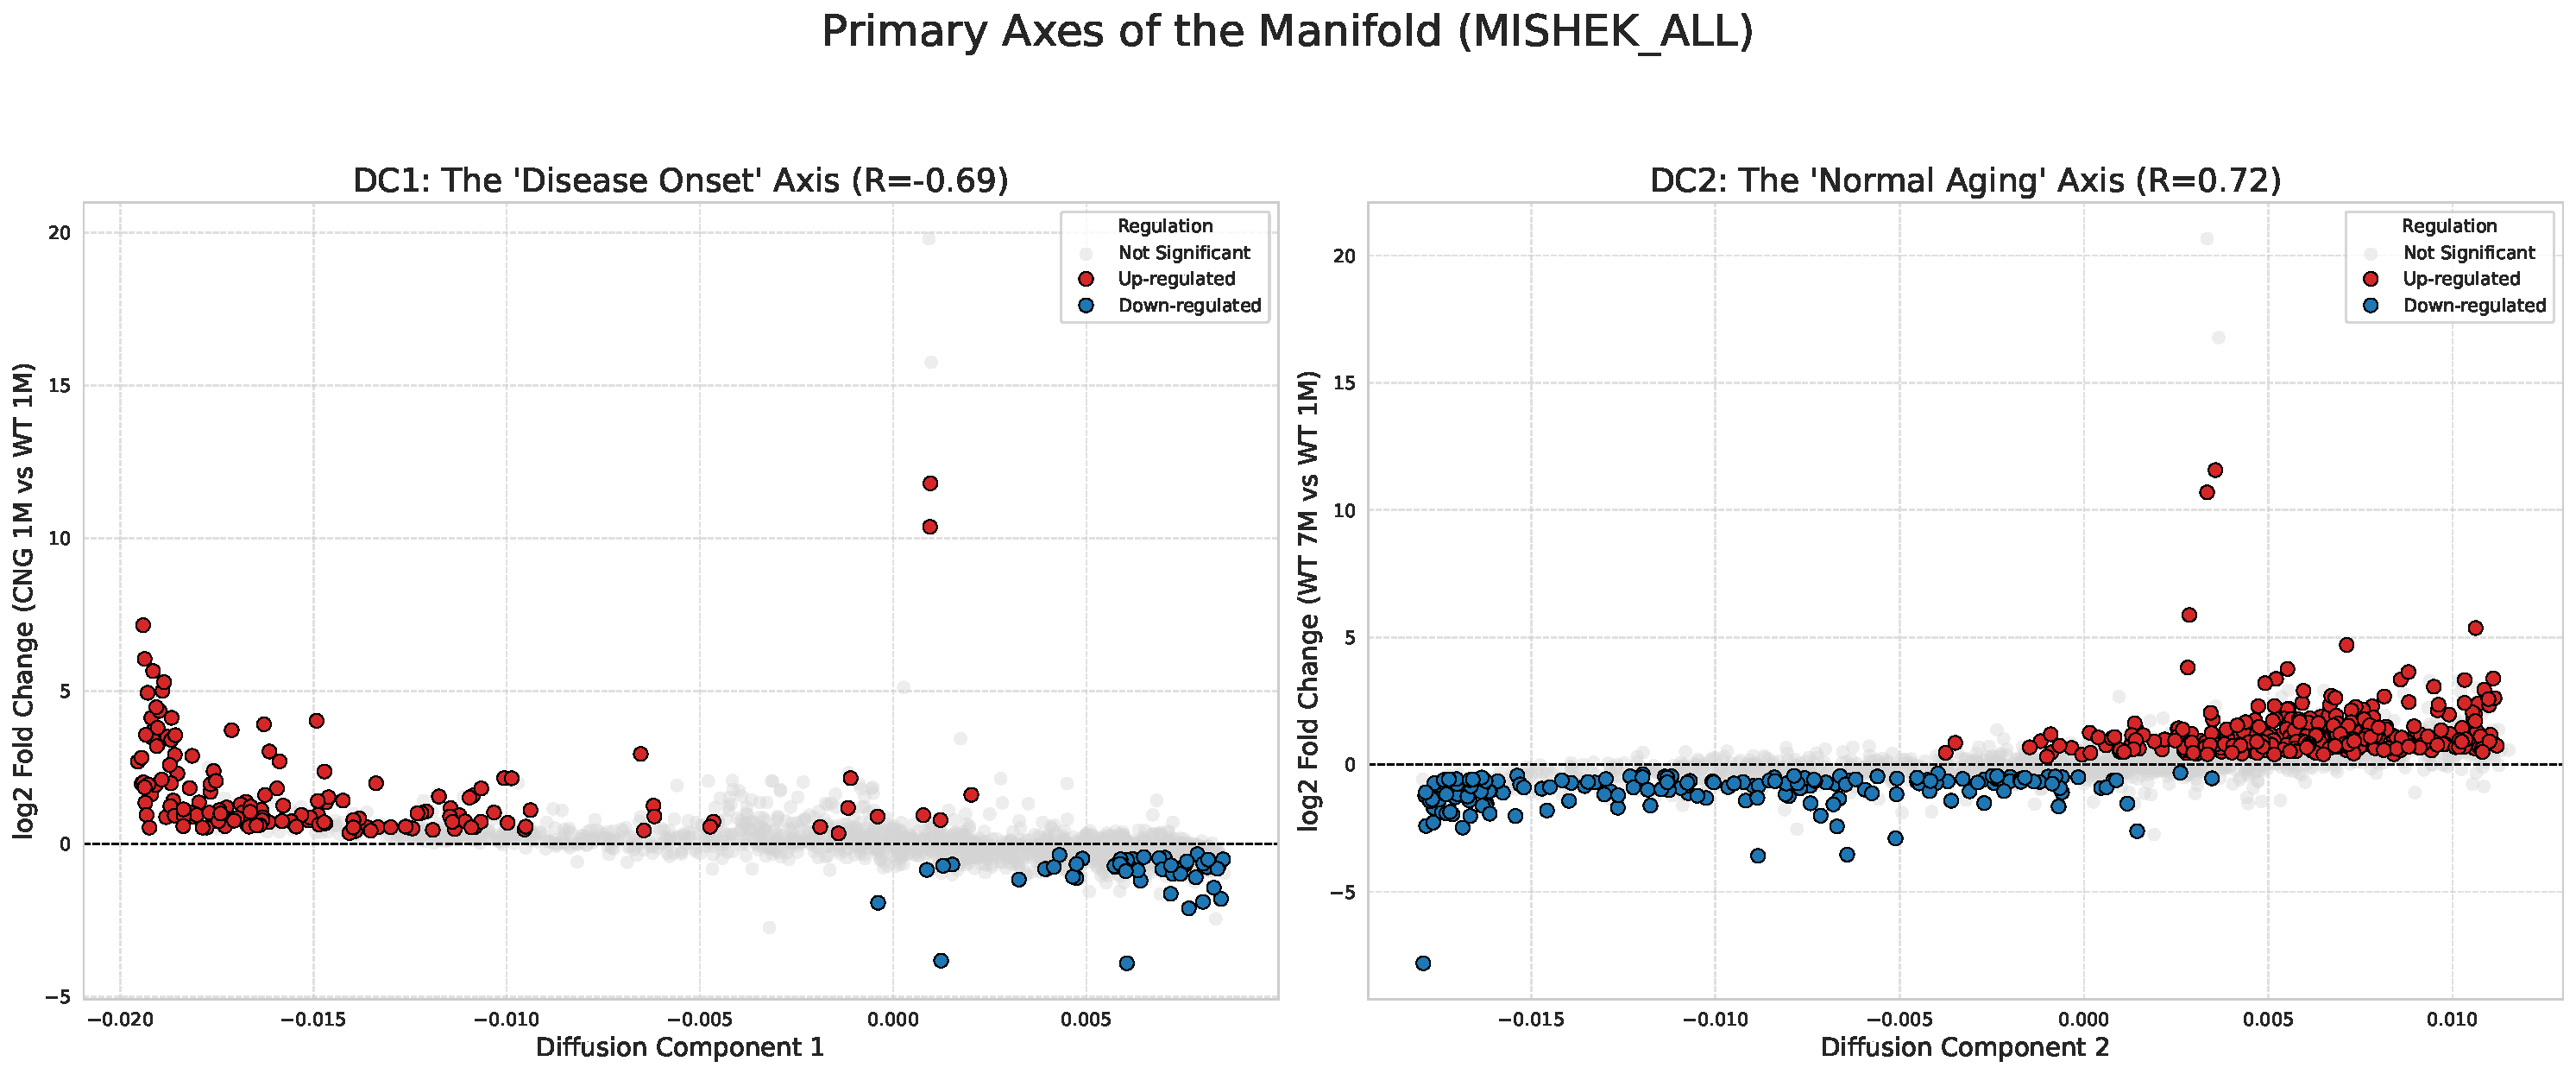
\includegraphics[width=\linewidth]{figures/mishek_all-primary_axes_interpretation_enhanced.pdf}
        \caption{Mishek - All Samples}
    \end{subfigure}
    \hfill
    \begin{subfigure}{0.49\textwidth}
        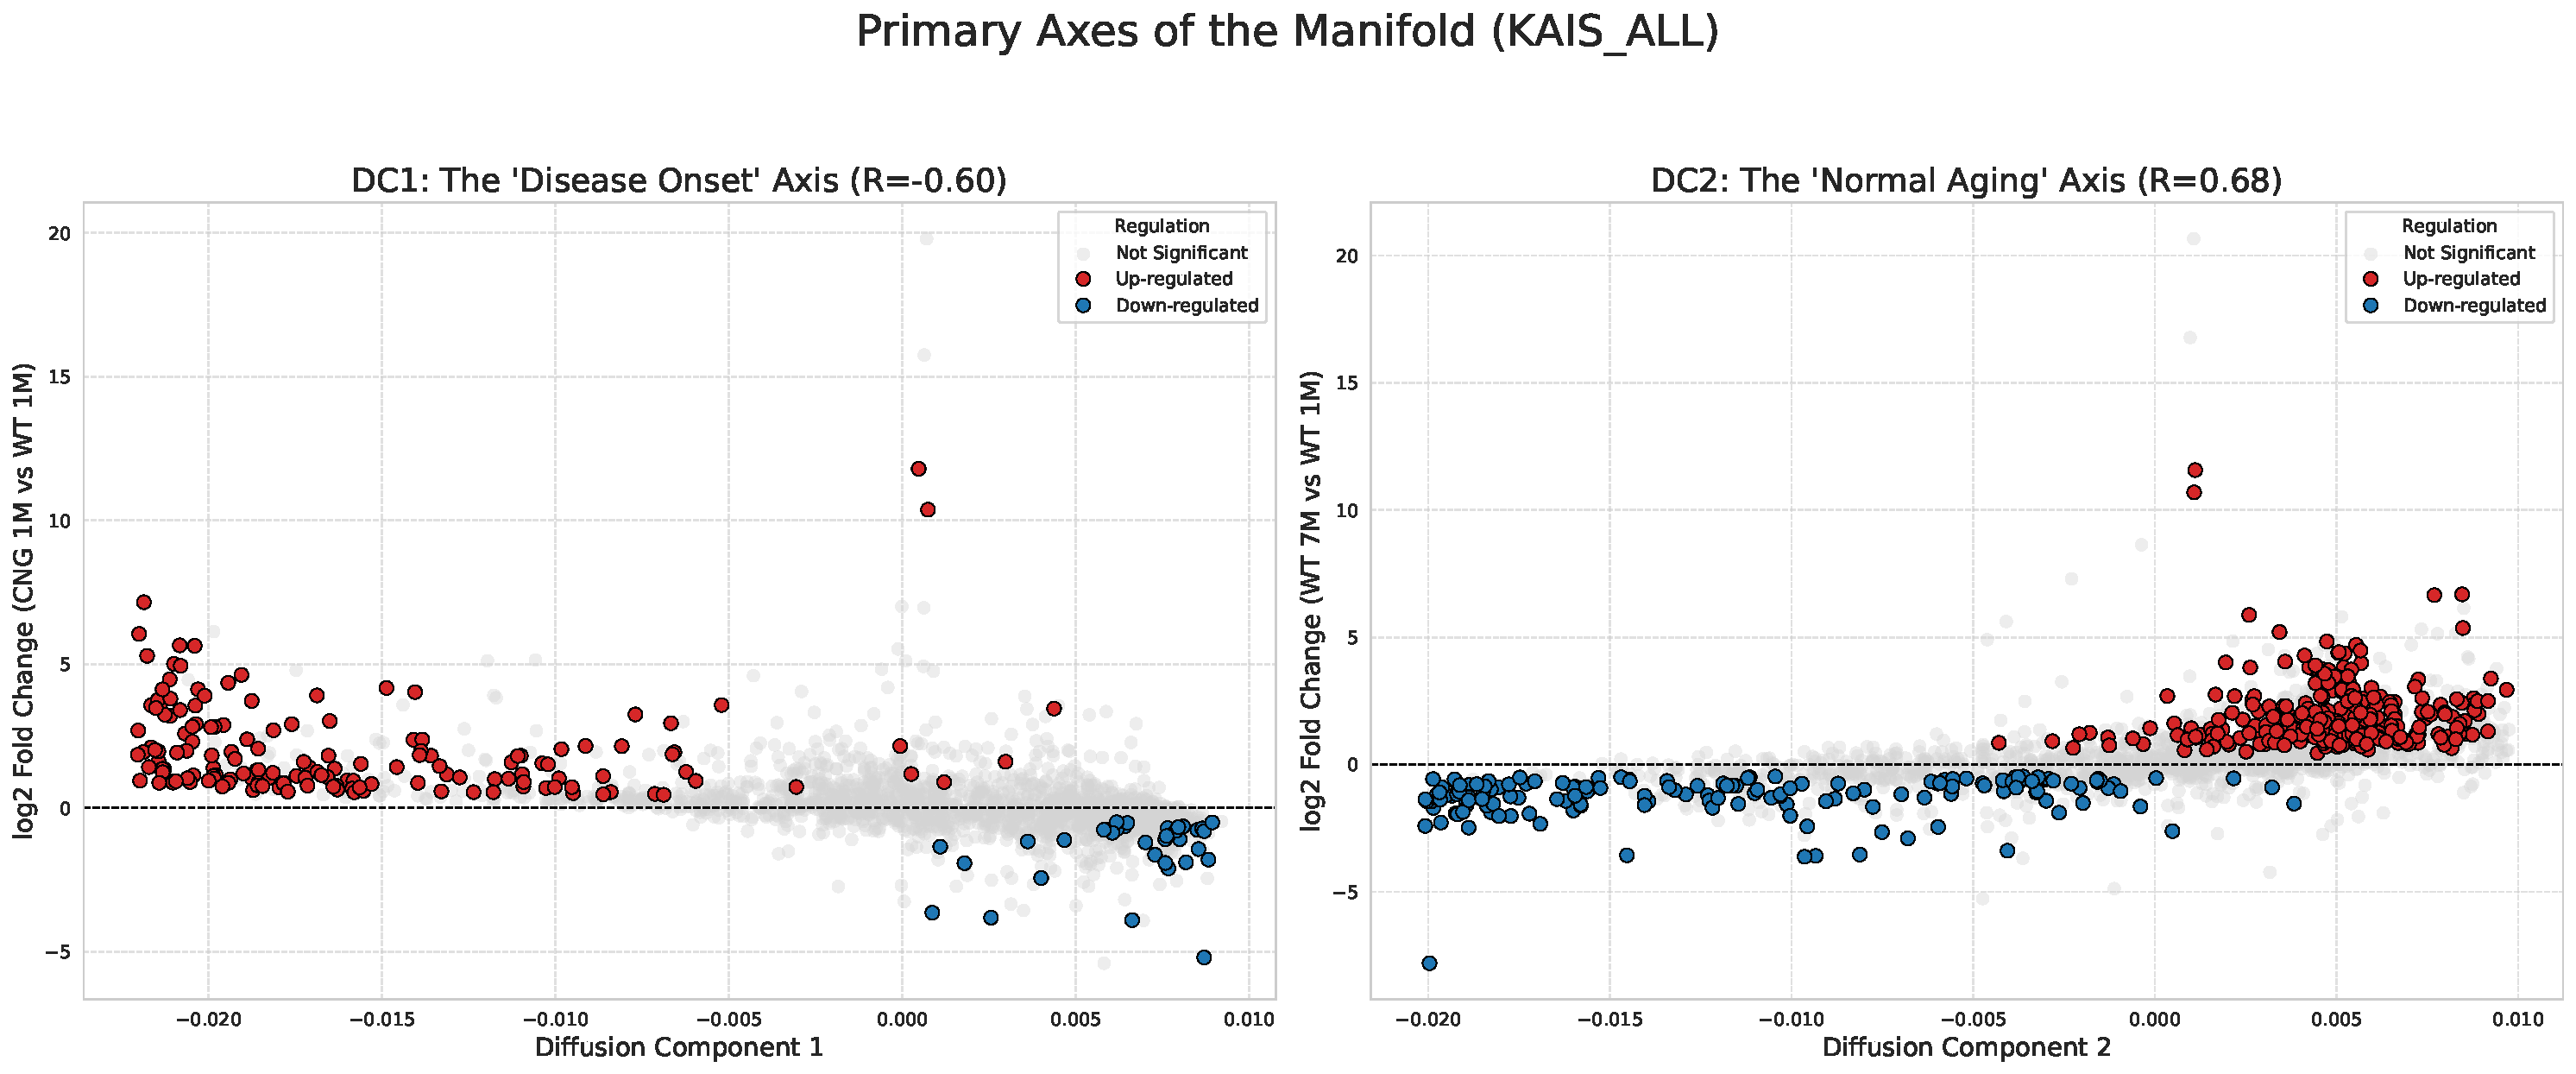
\includegraphics[width=\linewidth]{figures/kais_all-primary_axes_interpretation_enhanced.pdf}
        \caption{Kais - All Samples}
    \end{subfigure}
    
    \vspace{5mm}
    
    \begin{subfigure}{0.49\textwidth}
        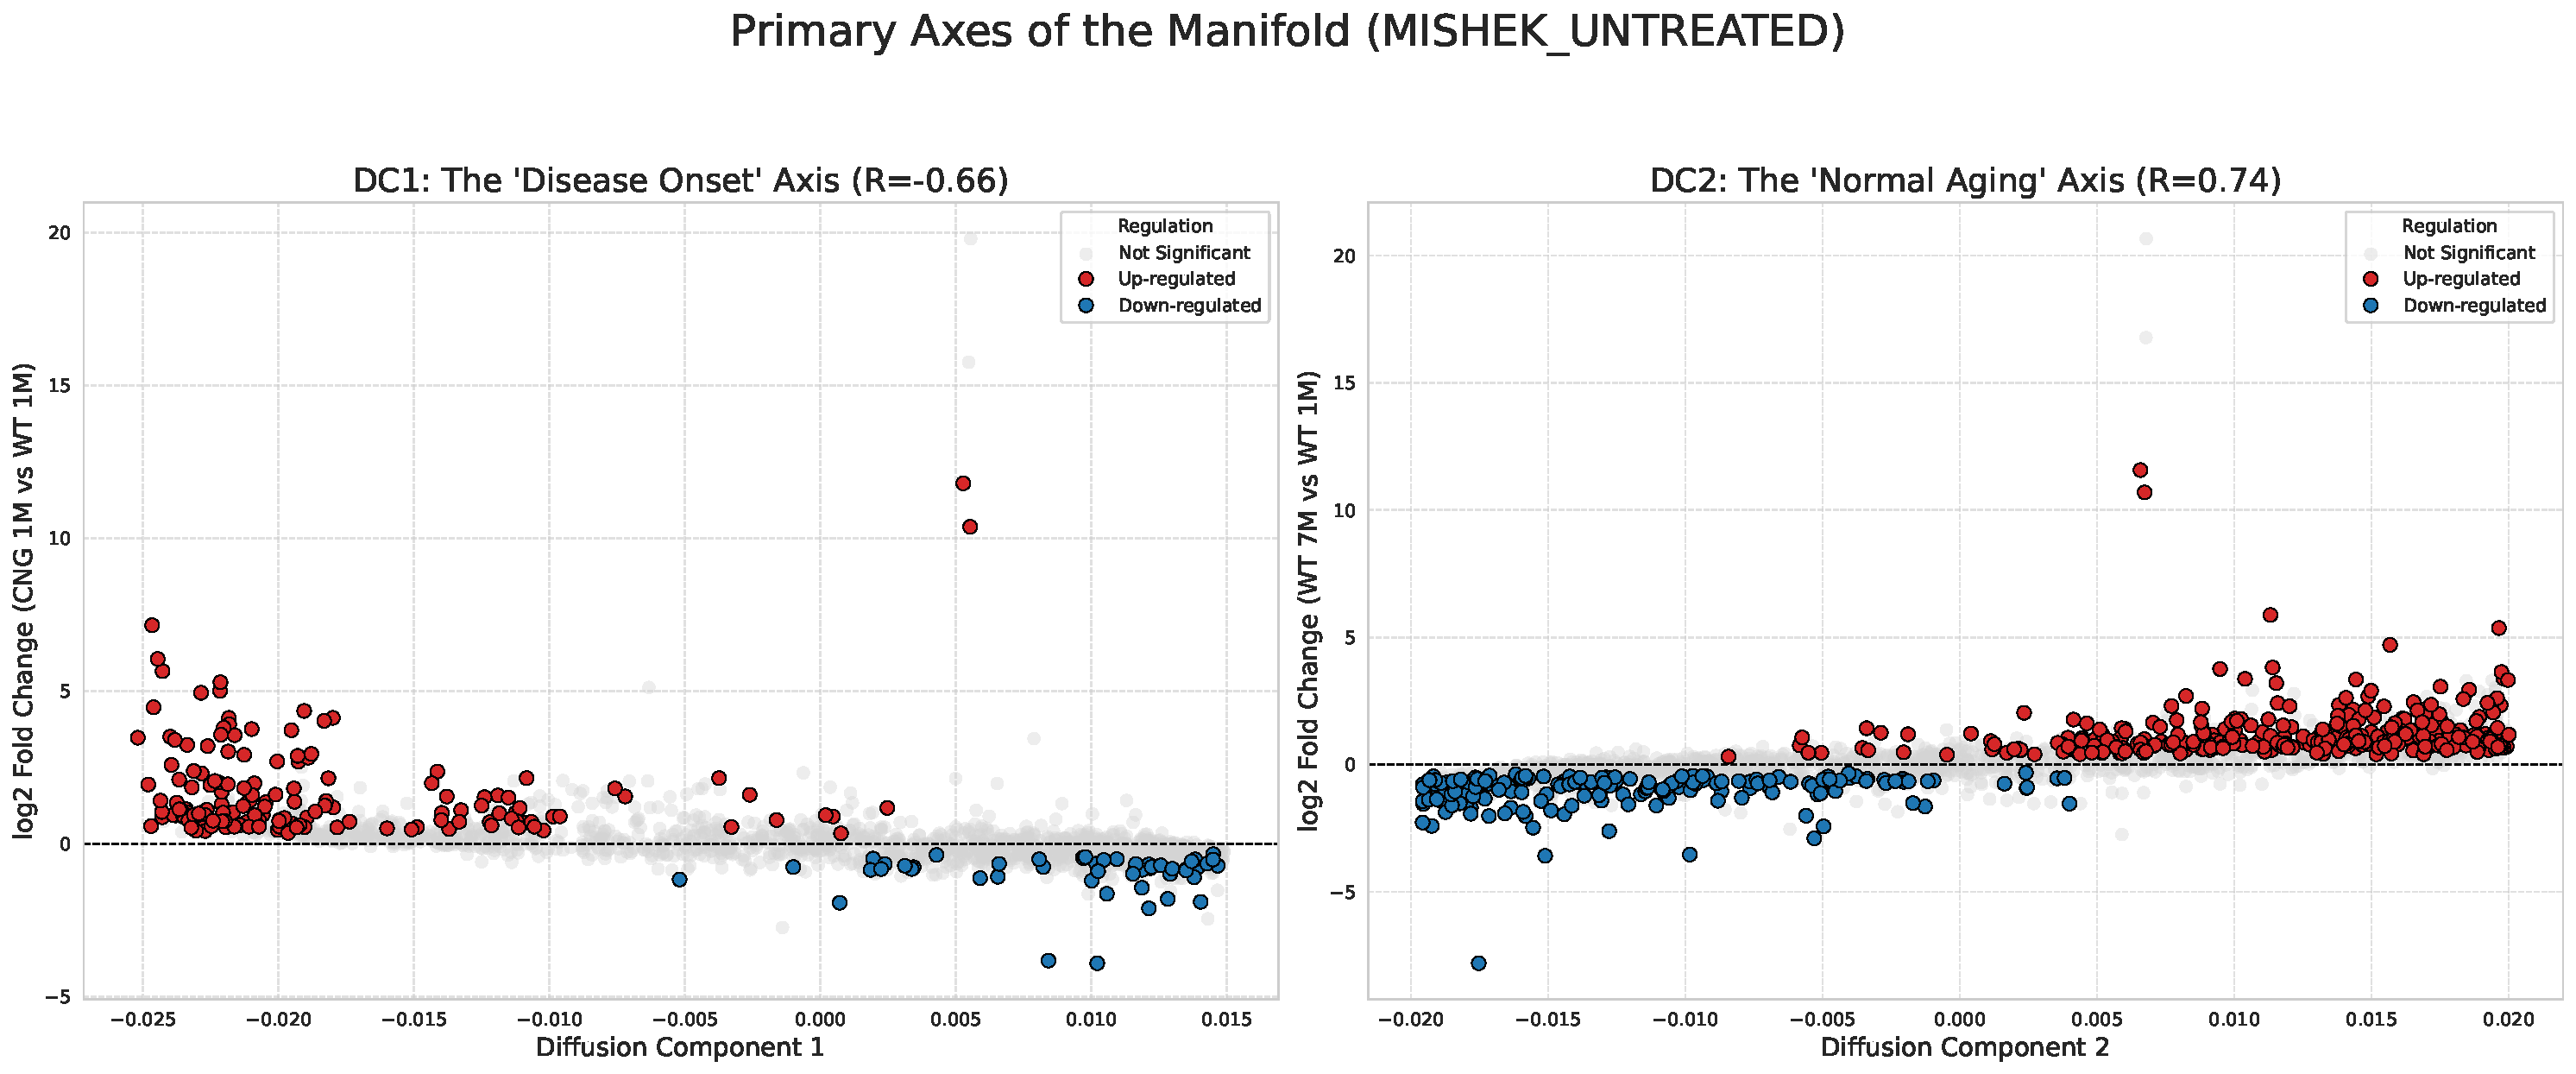
\includegraphics[width=\linewidth]{figures/mishek_untreated-primary_axes_interpretation_enhanced.pdf}
        \caption{Mishek - Untreated Only}
    \end{subfigure}
    \hfill
    \begin{subfigure}{0.49\textwidth}
        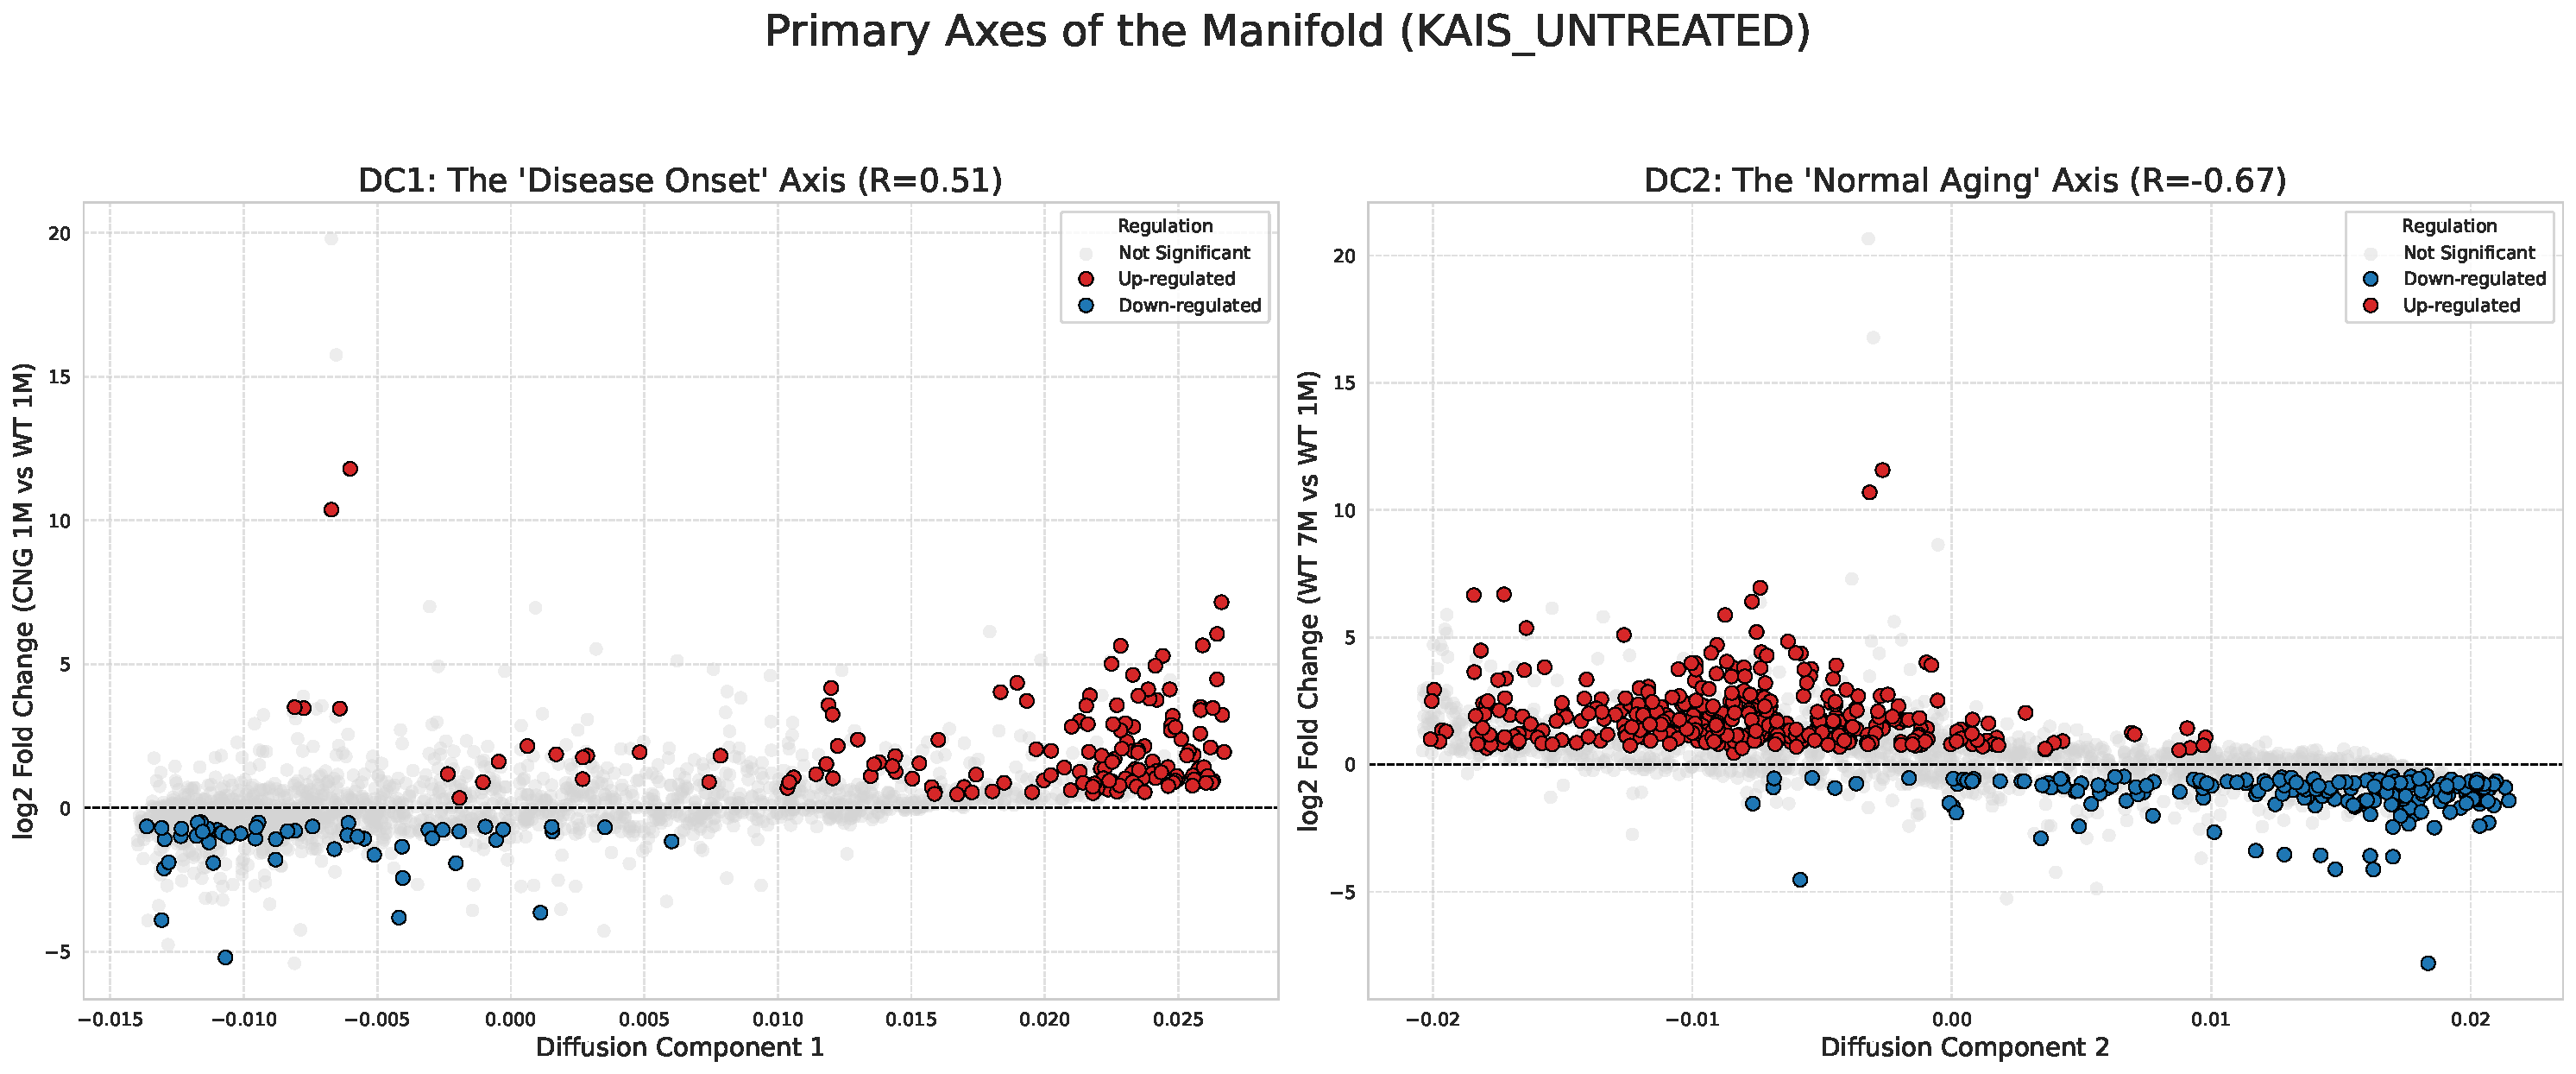
\includegraphics[width=\linewidth]{figures/kais_untreated-primary_axes_interpretation_enhanced.pdf}
        \caption{Kais - Untreated Only}
    \end{subfigure}
    \caption{Defining the Primary Manifold Axes. DC1 represents the 'Disease Onset Axis' and DC2 represents the 'Normal Aging Axis' across all analysis versions.}
    \label{fig:primary_axes_all_versions}
\end{figure}

\begin{figure}[htbp]
    \centering
    \begin{subfigure}{0.49\textwidth}
        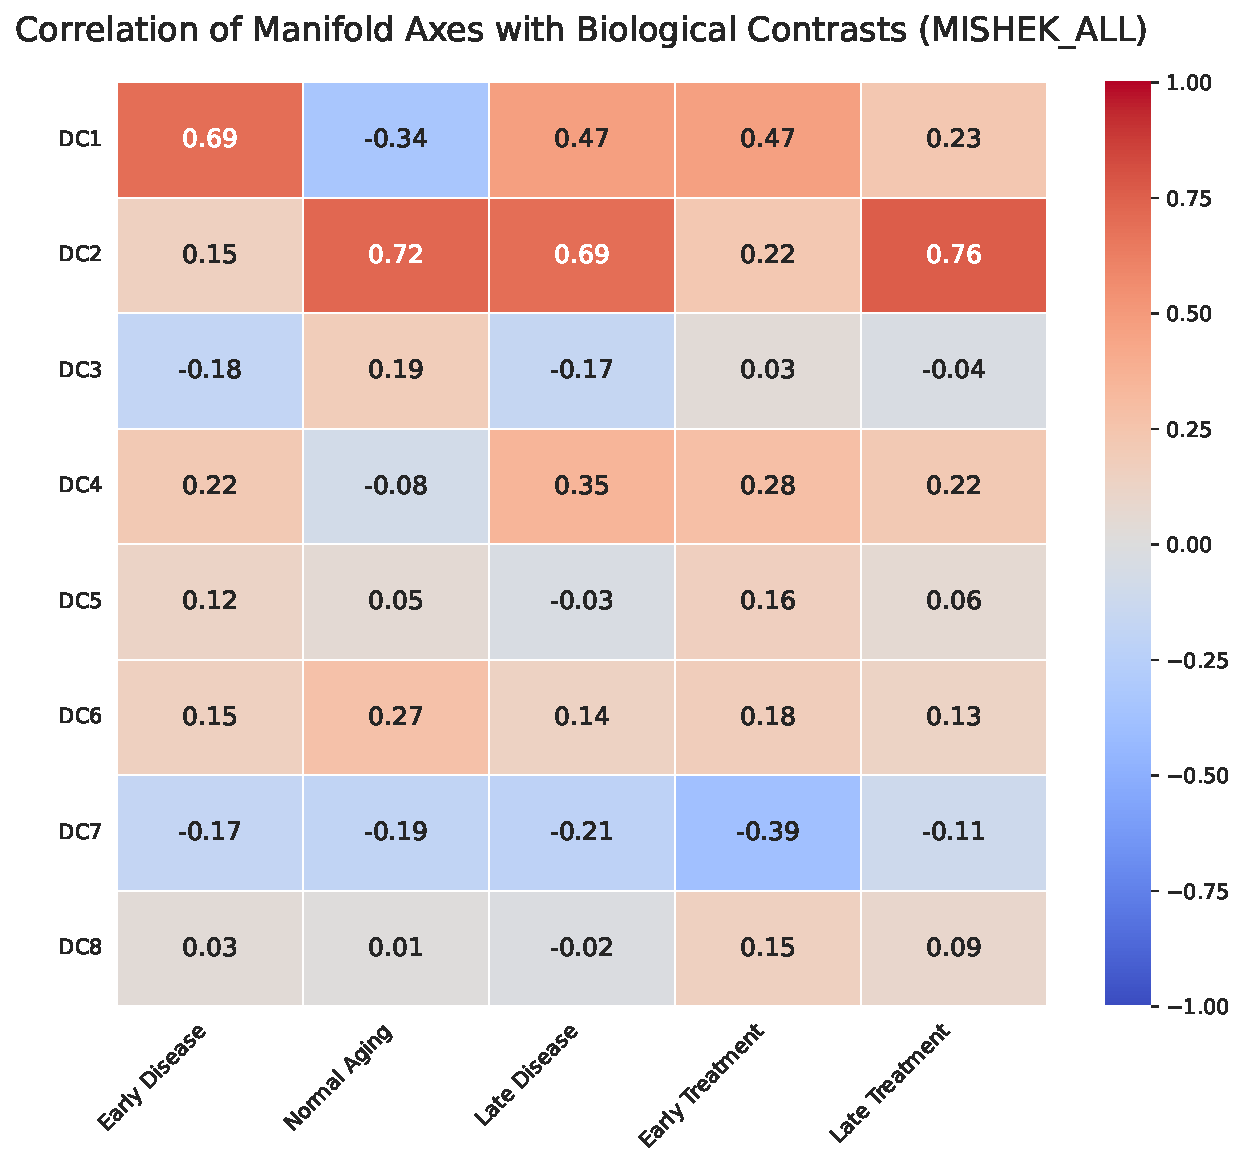
\includegraphics[width=\linewidth]{figures/mishek_allcorrelation_heatmap.pdf}
        \caption{Mishek - All Samples}
    \end{subfigure}
    \hfill
    \begin{subfigure}{0.49\textwidth}
        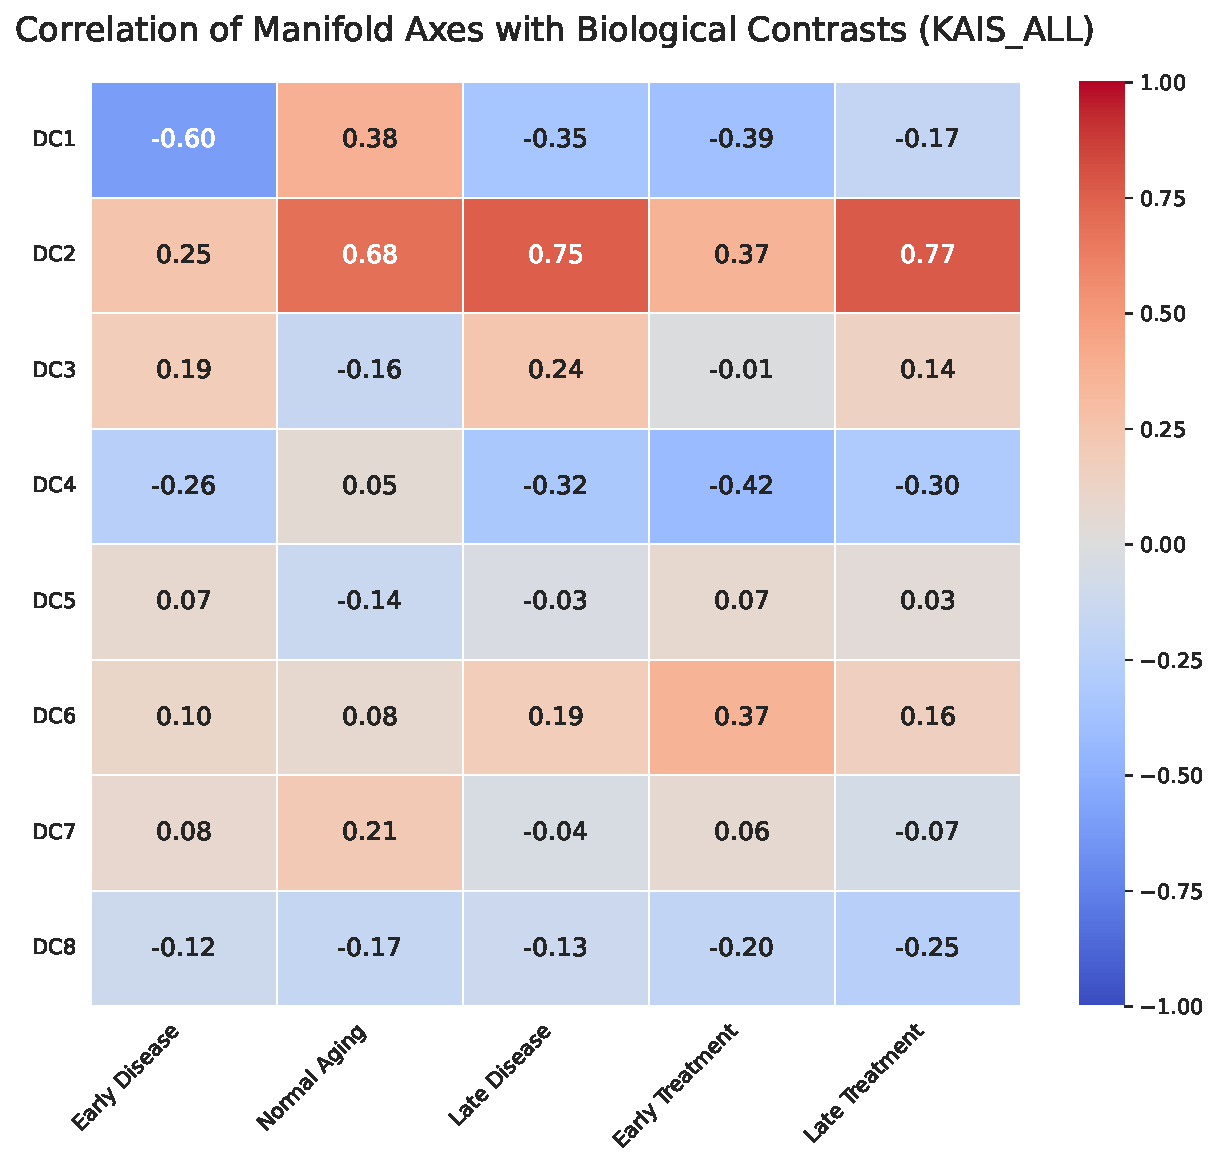
\includegraphics[width=\linewidth]{figures/kais_all-correlation_heatmap.pdf}
        \caption{Kais - All Samples}
    \end{subfigure}
    
    \vspace{5mm}
    
    \begin{subfigure}{0.49\textwidth}
        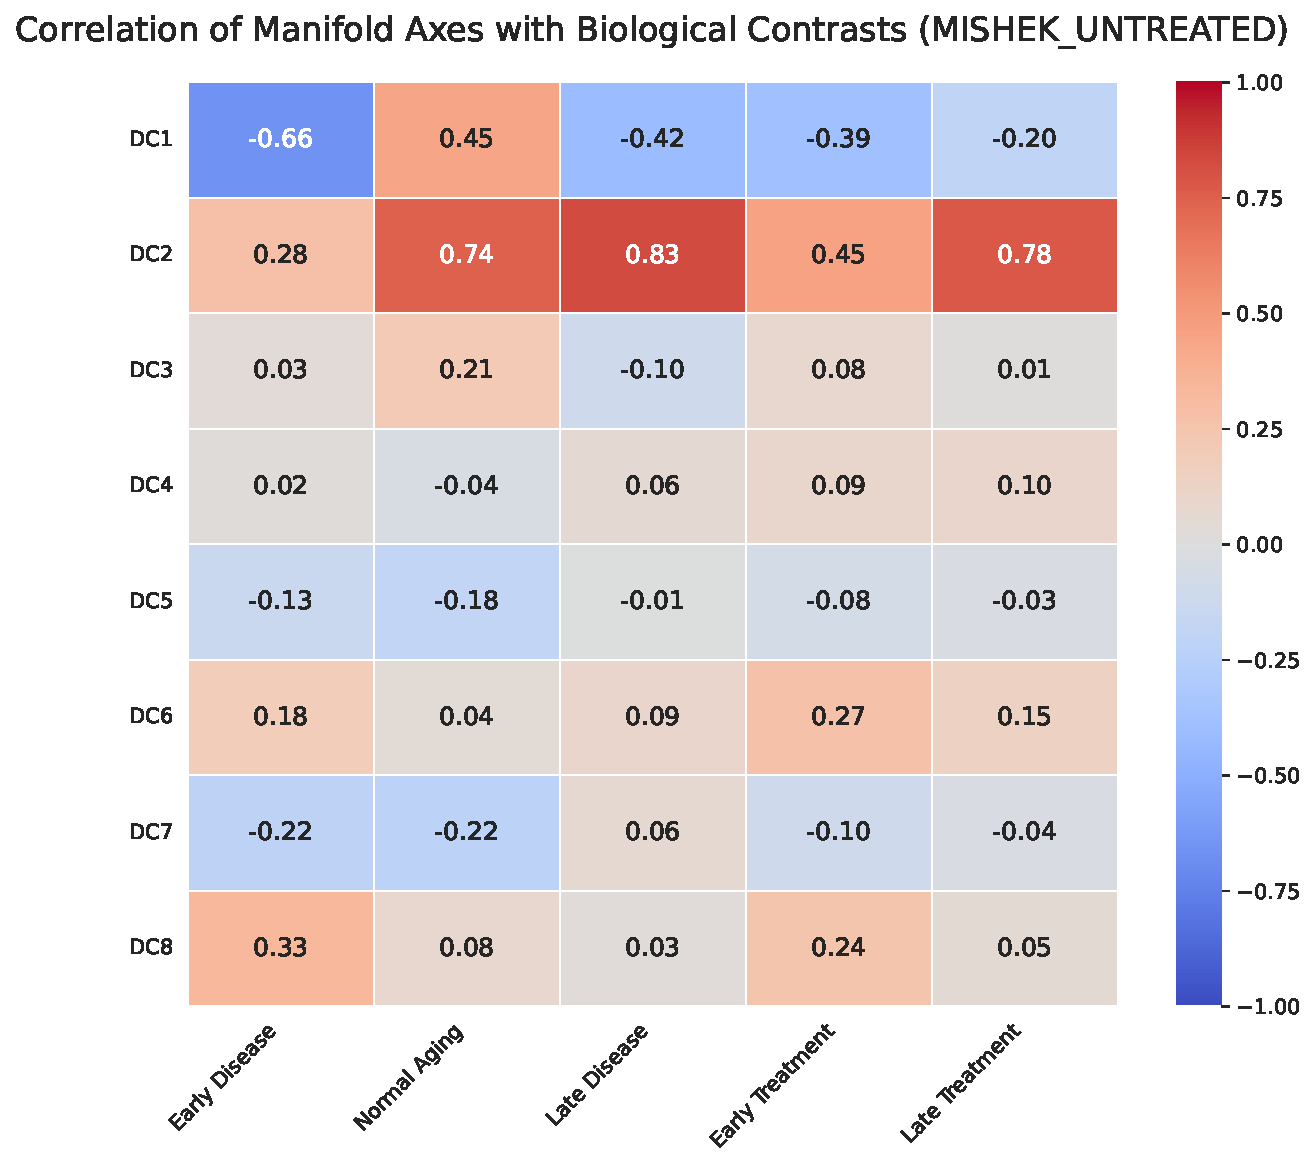
\includegraphics[width=\linewidth]{figures/mishek_untreated-correlation_heatmap.pdf}
        \caption{Mishek - Untreated Only}
    \end{subfigure}
    \hfill
    \begin{subfigure}{0.49\textwidth}
        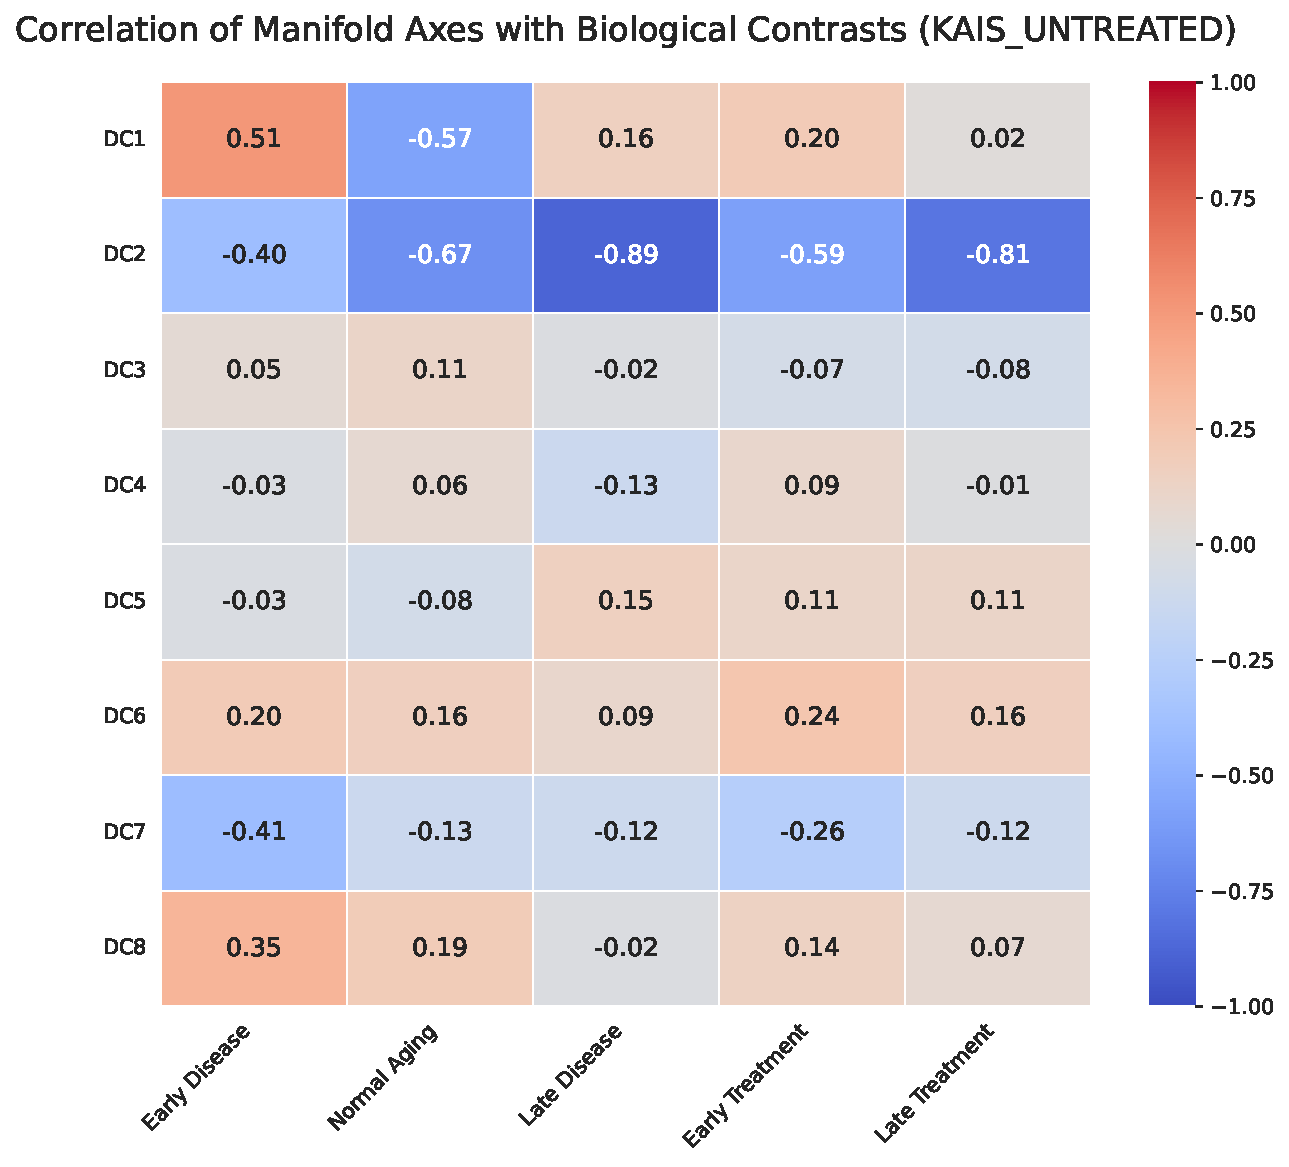
\includegraphics[width=\linewidth]{figures/kais_untreated-correlation_heatmap.pdf}
        \caption{Kais - Untreated Only}
    \end{subfigure}
    \caption{Correlation of diffusion components with biological contrasts across all analysis versions.}
    \label{fig:correlation_heatmaps_all_versions}
\end{figure}

\begin{figure}[htbp]
    \centering
    \begin{subfigure}{0.49\textwidth}
        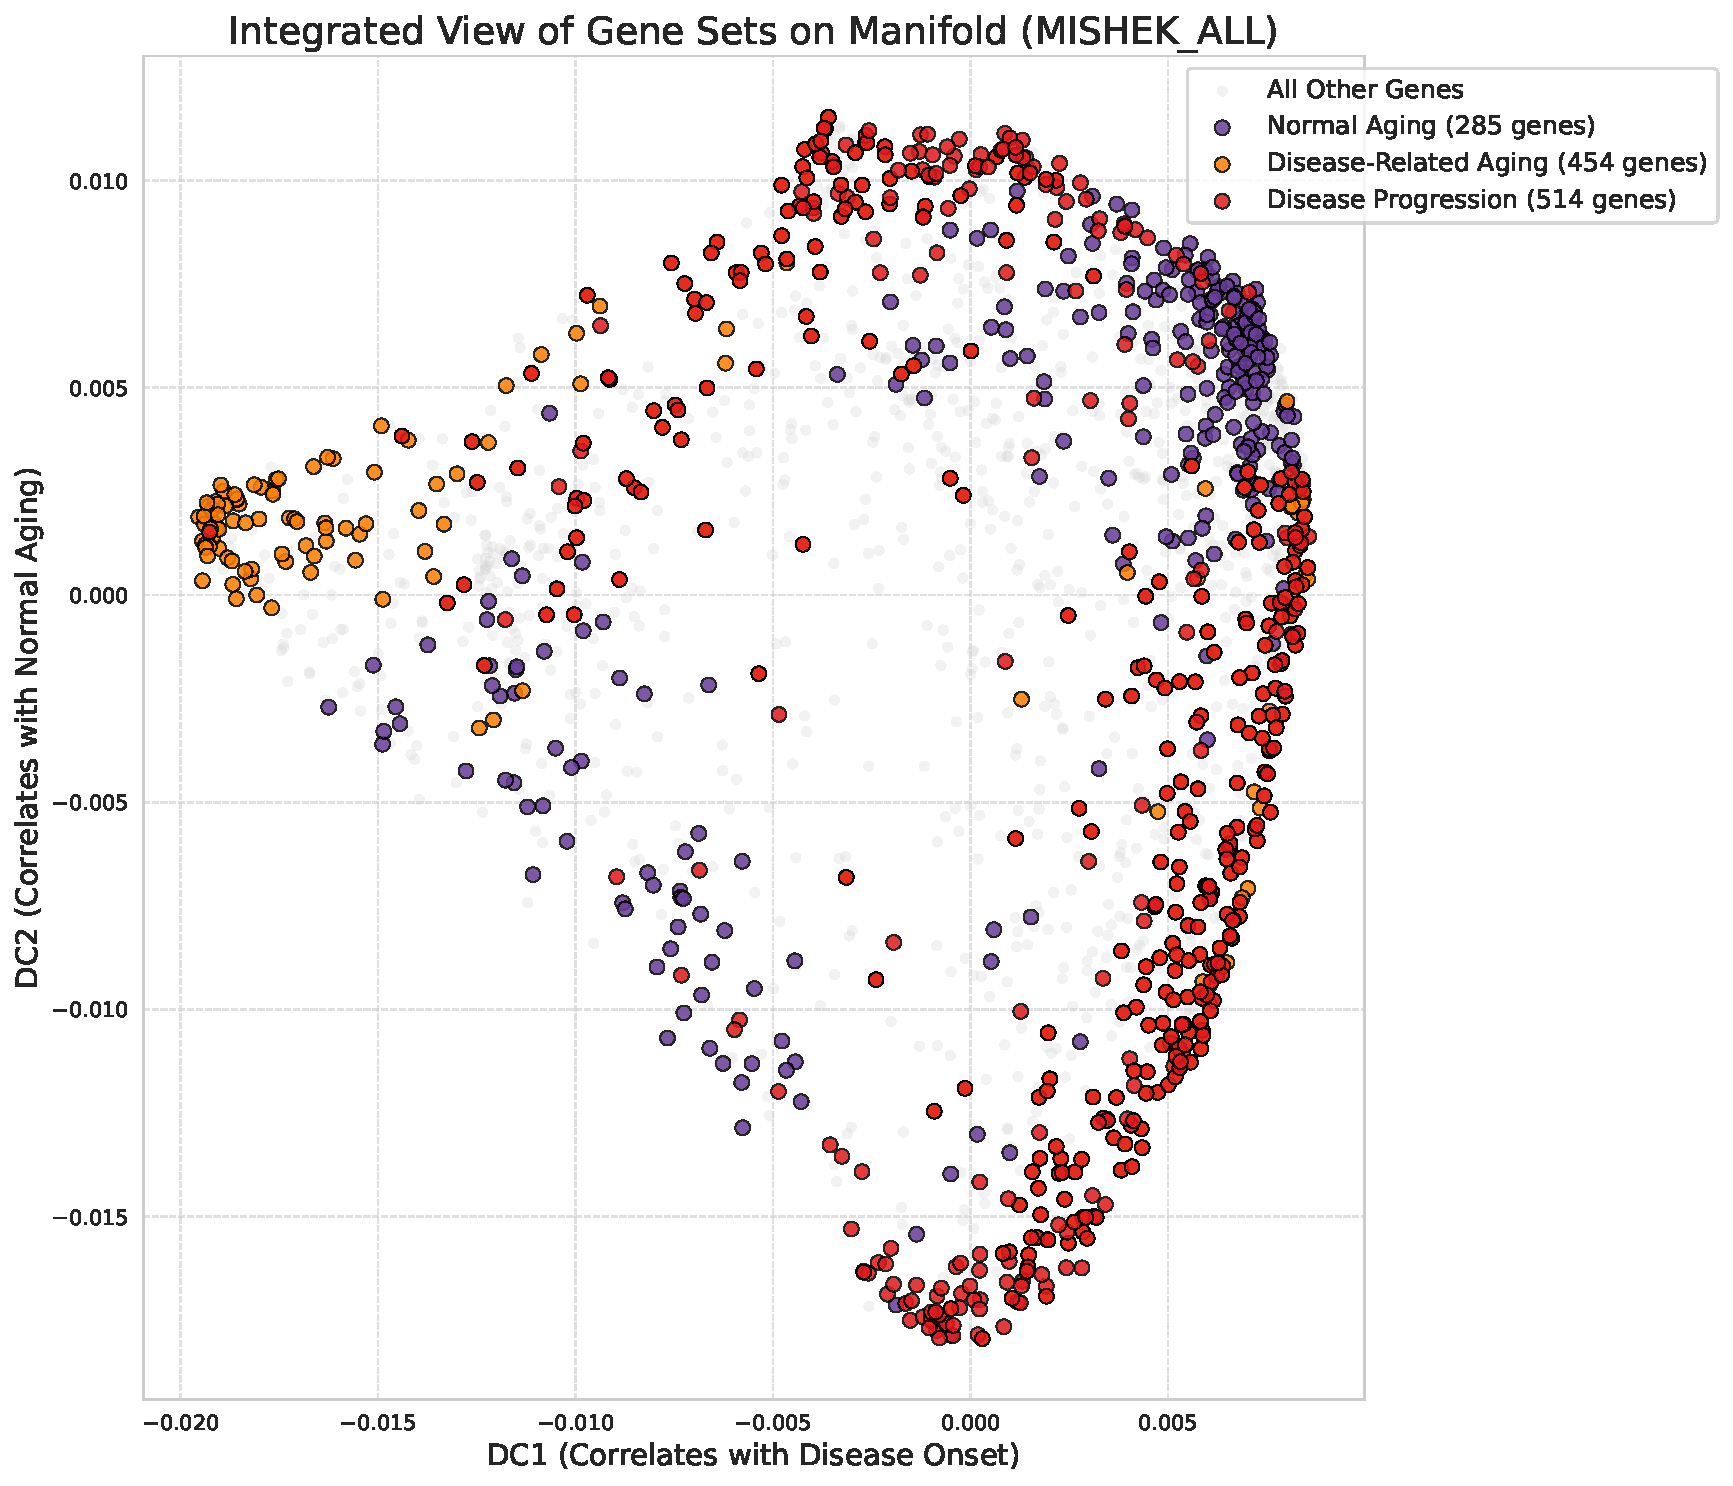
\includegraphics[width=\linewidth]{figures/mishek_all-integrated_gene_sets.pdf}
        \caption{Mishek - All Samples}
    \end{subfigure}
    \hfill
    \begin{subfigure}{0.49\textwidth}
        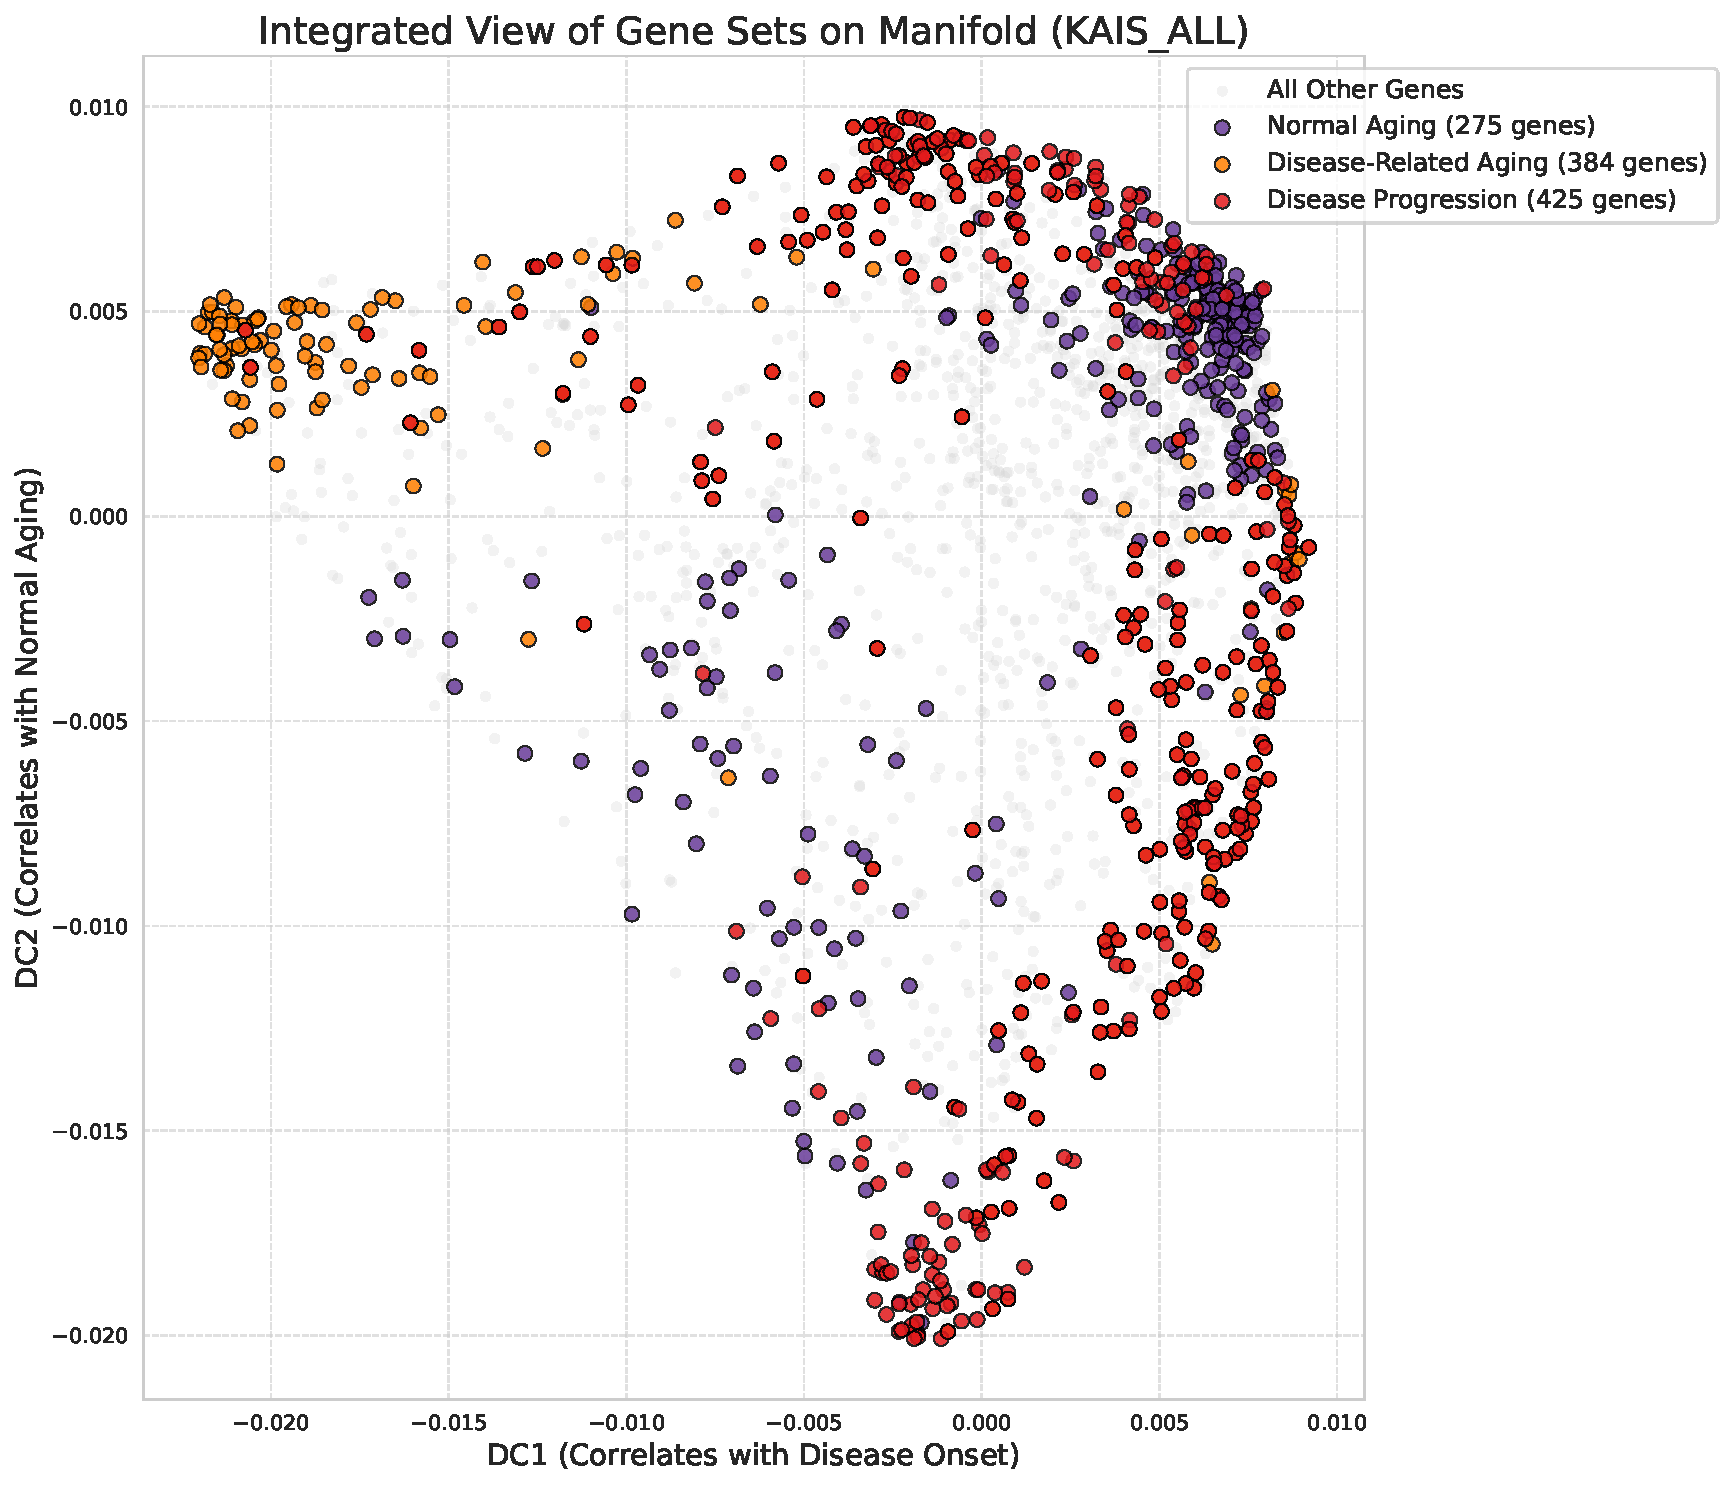
\includegraphics[width=\linewidth]{figures/kais_all-integrated_gene_sets.pdf}
        \caption{Kais - All Samples}
    \end{subfigure}
    
    \vspace{5mm}
    
    \begin{subfigure}{0.49\textwidth}
        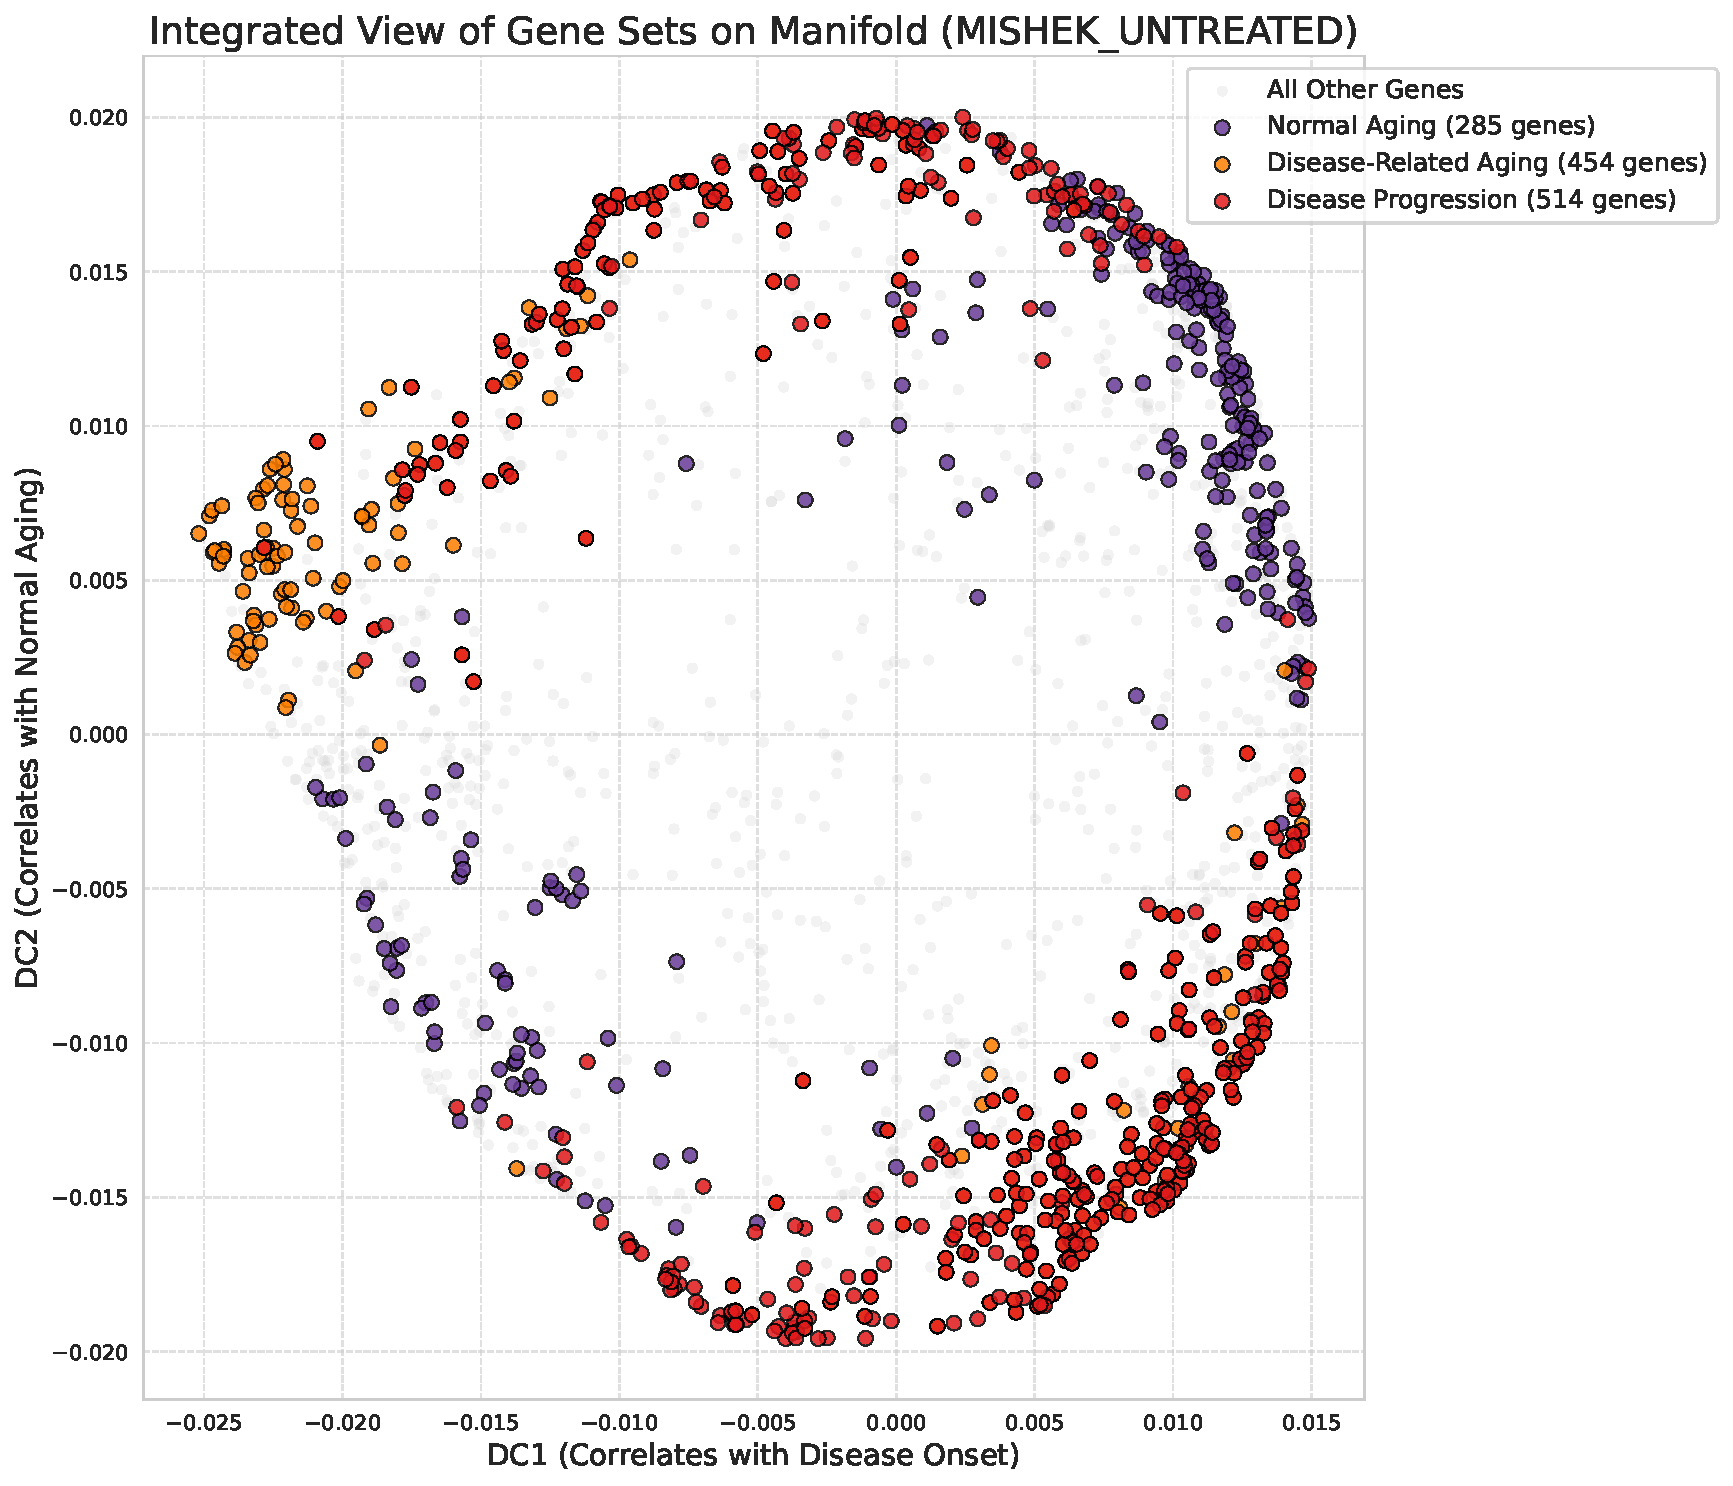
\includegraphics[width=\linewidth]{figures/mishek_untreated-integrated_gene_sets.pdf}
        \caption{Mishek - Untreated Only}
    \end{subfigure}
    \hfill
    \begin{subfigure}{0.49\textwidth}
        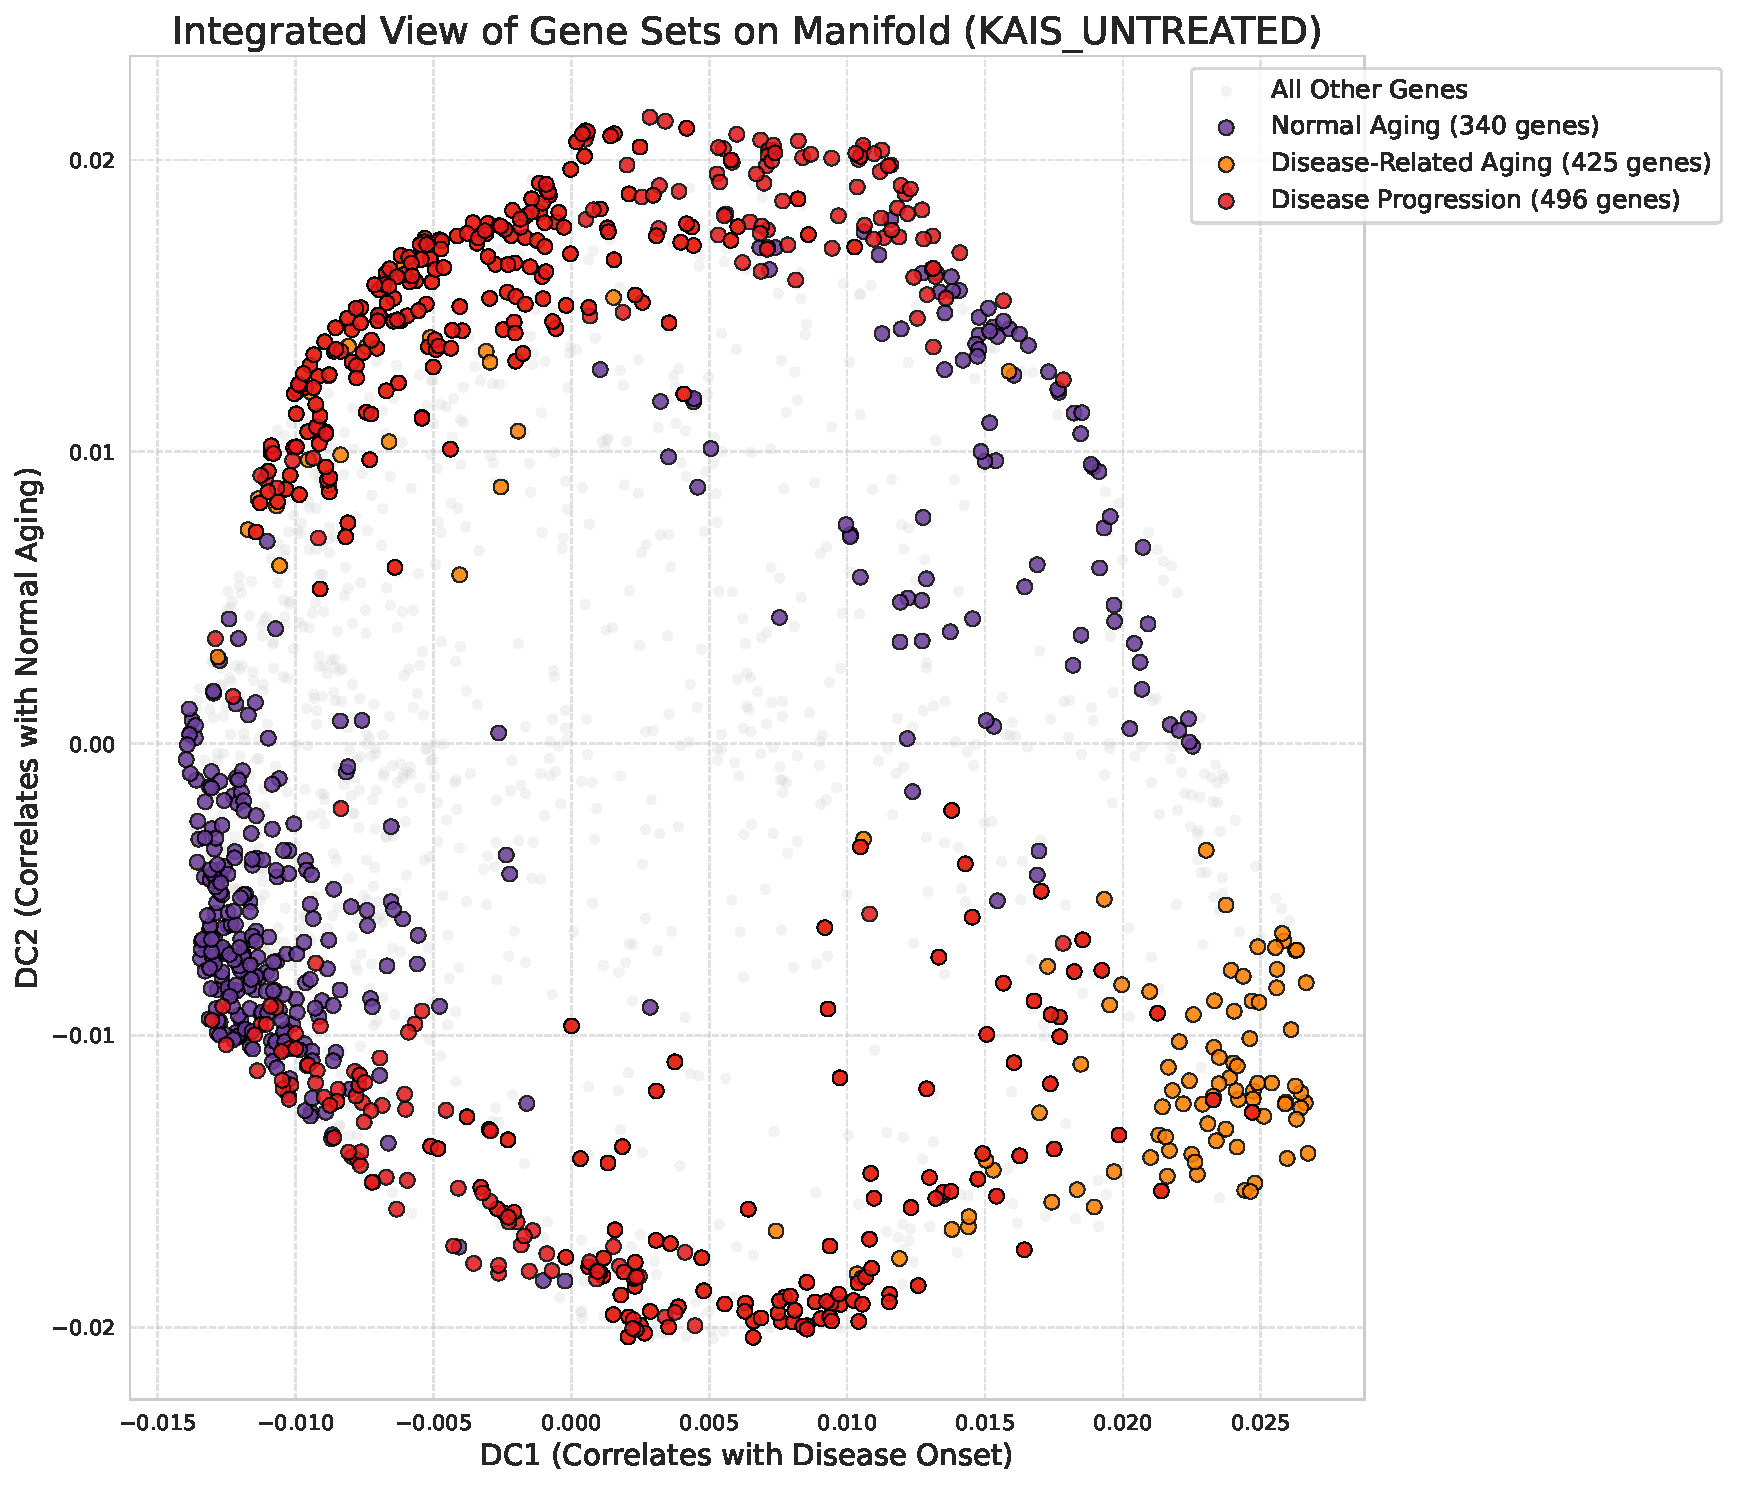
\includegraphics[width=\linewidth]{figures/kais_untreated-integrated_gene_sets.pdf}
        \caption{Kais - Untreated Only}
    \end{subfigure}
    \caption{Integrated view of gene sets on the manifold across all analysis versions.}
    \label{fig:integrated_view_all_versions}
\end{figure}

\begin{figure}[htbp]
    \centering
    \begin{subfigure}{\textwidth}
        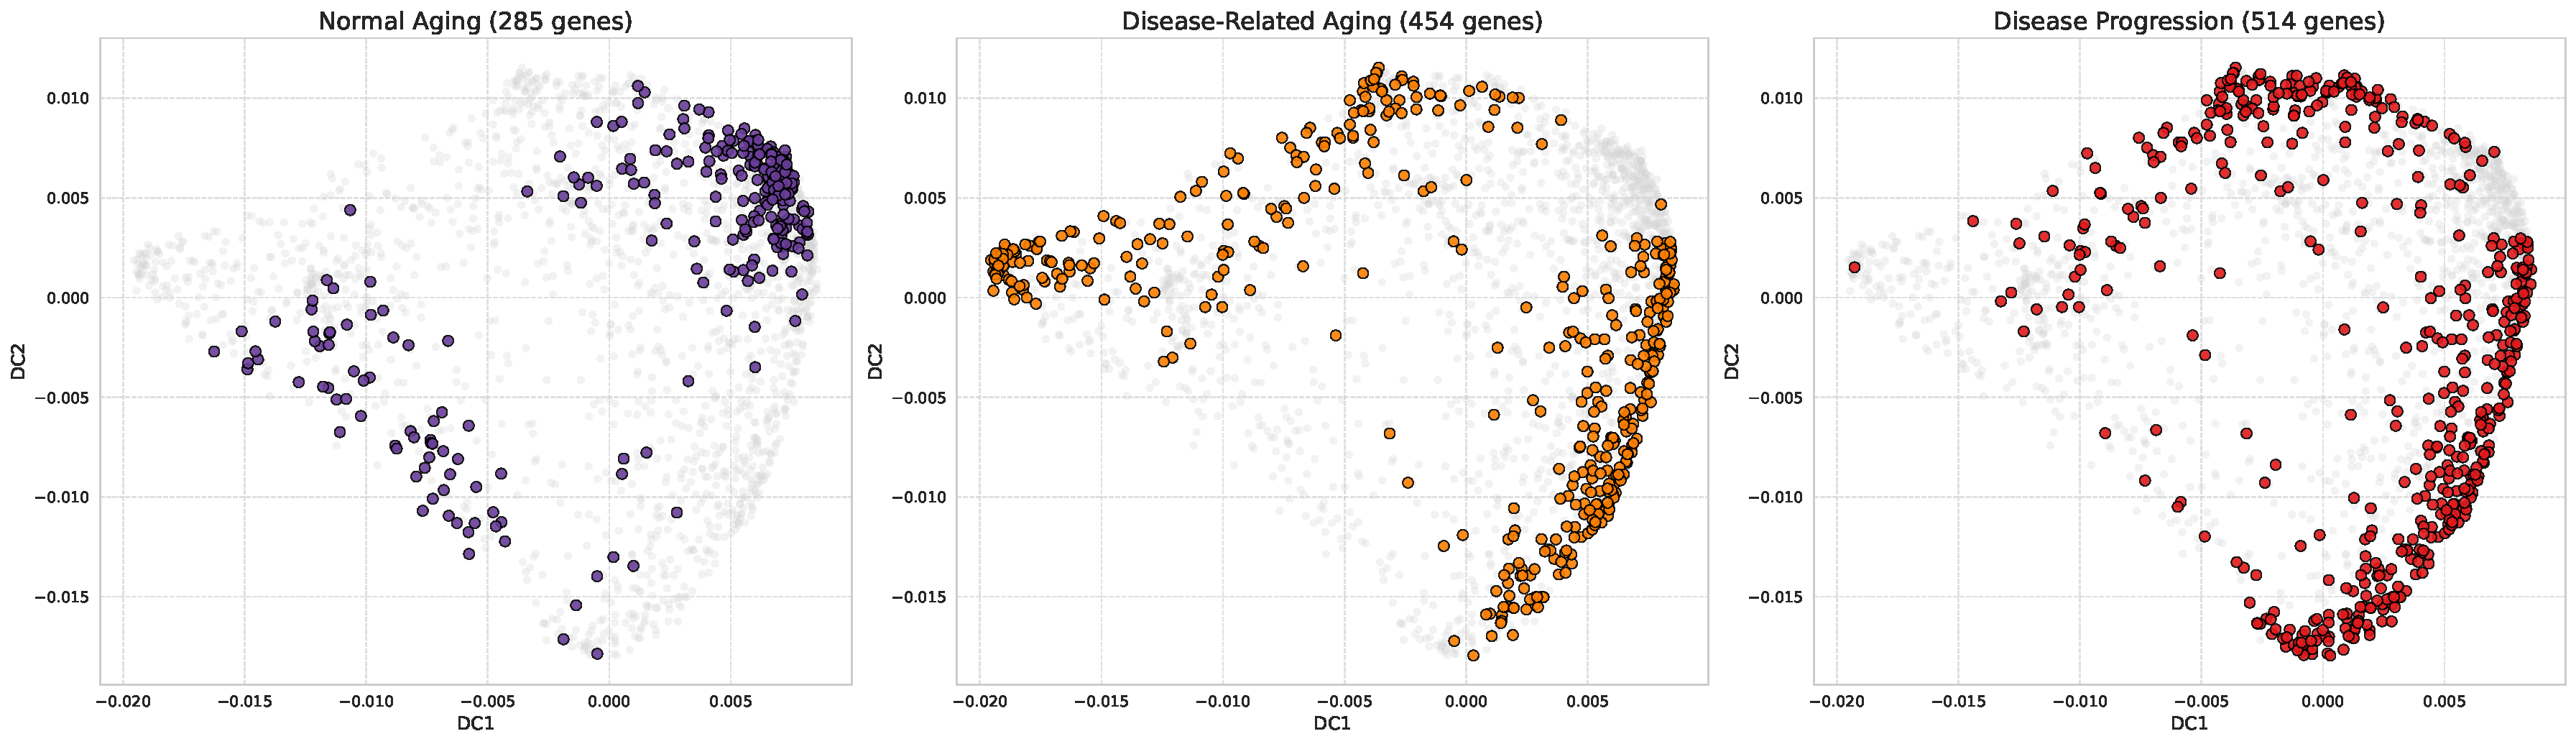
\includegraphics[width=\linewidth]{figures/mishek_all-multi_panel_gene_sets.pdf}
        \caption{Mishek - All Samples}
    \end{subfigure}
    
    \vspace{5mm}
    
    \begin{subfigure}{\textwidth}
        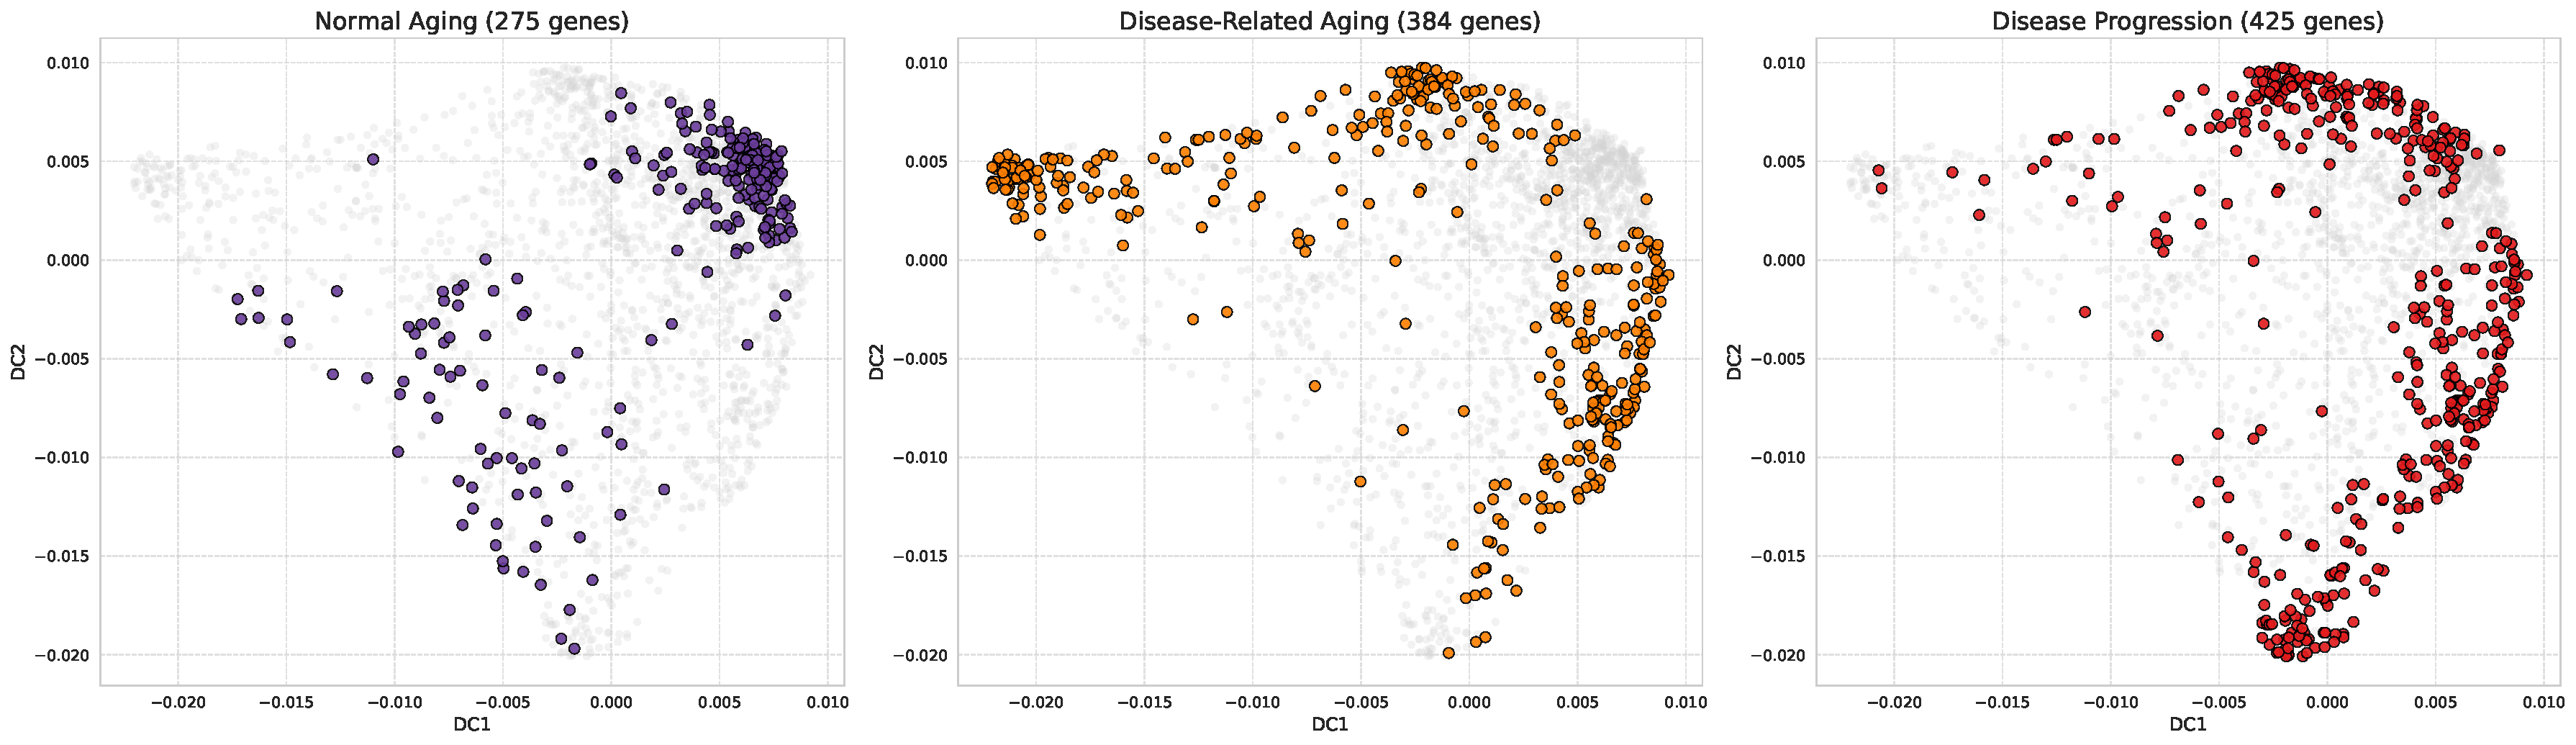
\includegraphics[width=\linewidth]{figures/kais_all-multi_panel_gene_sets.pdf}
        \caption{Kais - All Samples}
    \end{subfigure}
    \caption{Multi-panel visualization of gene sets for the analyses including all samples (treated and untreated).}
    \label{fig:multipanel_all_samples}
\end{figure}

\begin{figure}[htbp]
    \centering
    \begin{subfigure}{\textwidth}
        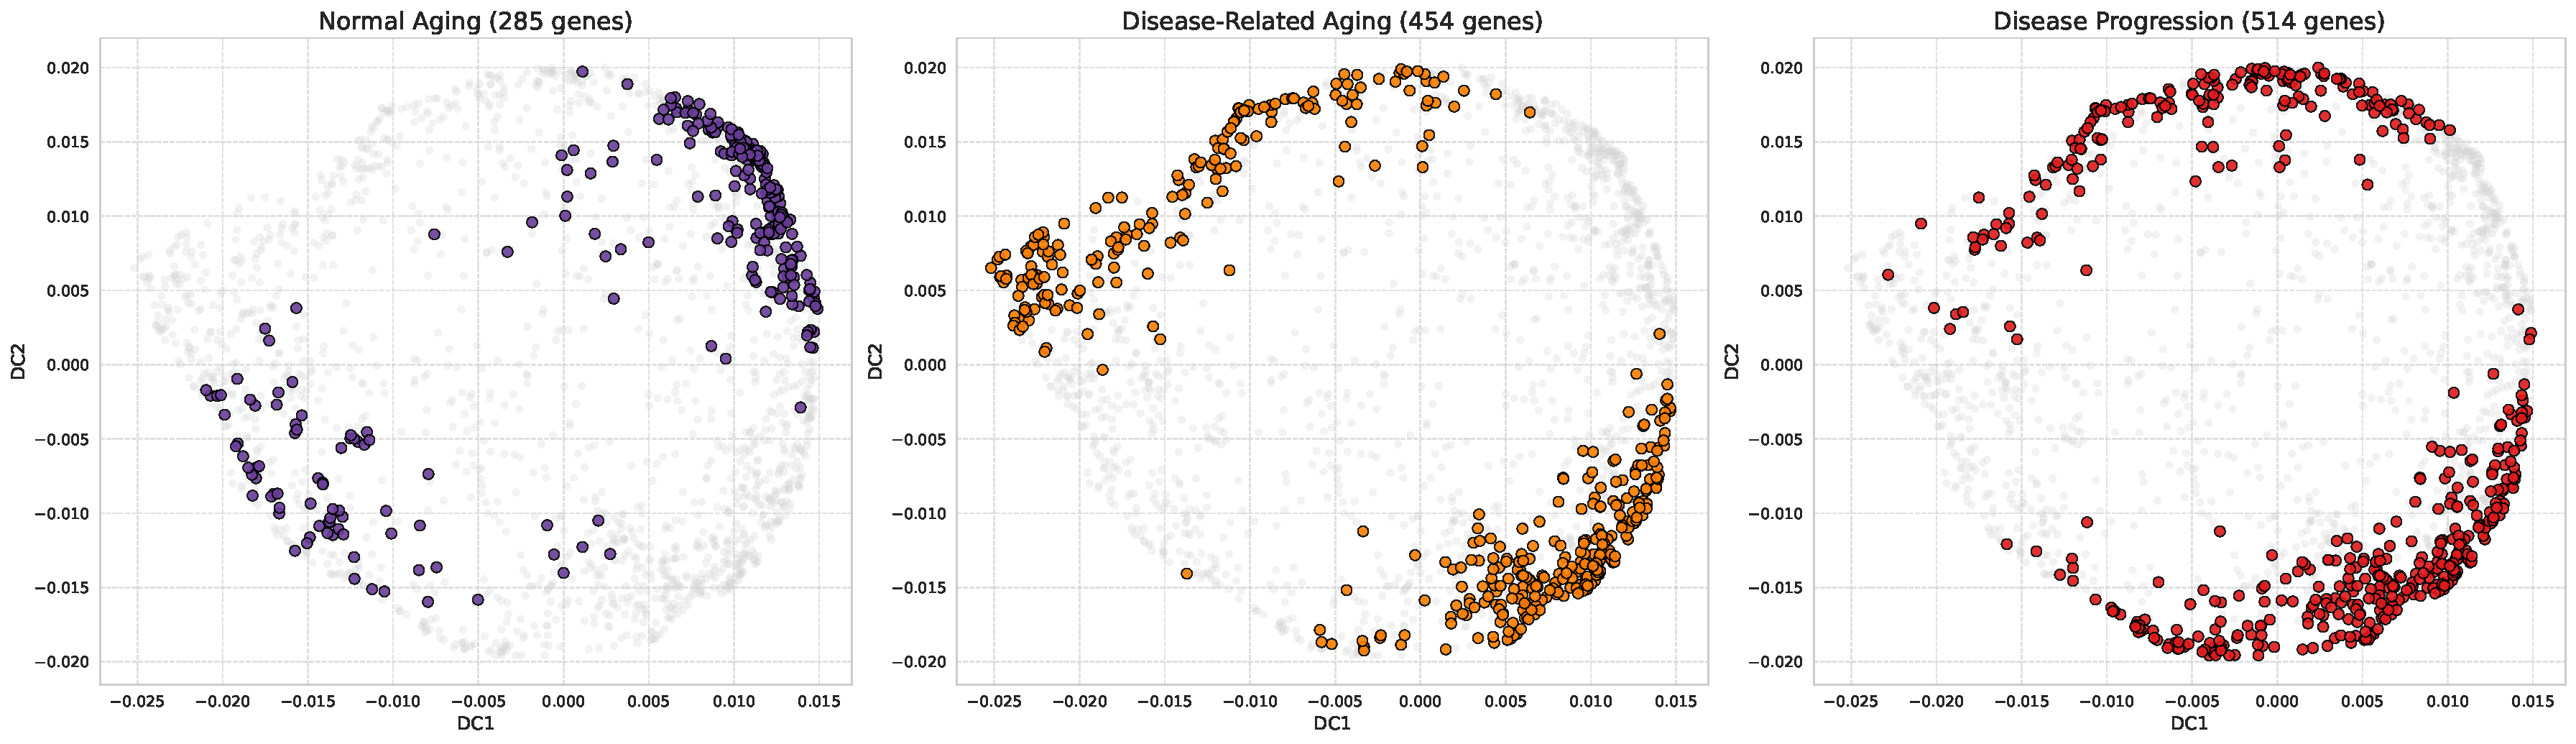
\includegraphics[width=\linewidth]{figures/mishek_untreated-multi_panel_gene_sets.pdf}
        \caption{Mishek - Untreated Only}
    \end{subfigure}
    
    \vspace{5mm}
    
    \begin{subfigure}{\textwidth}
        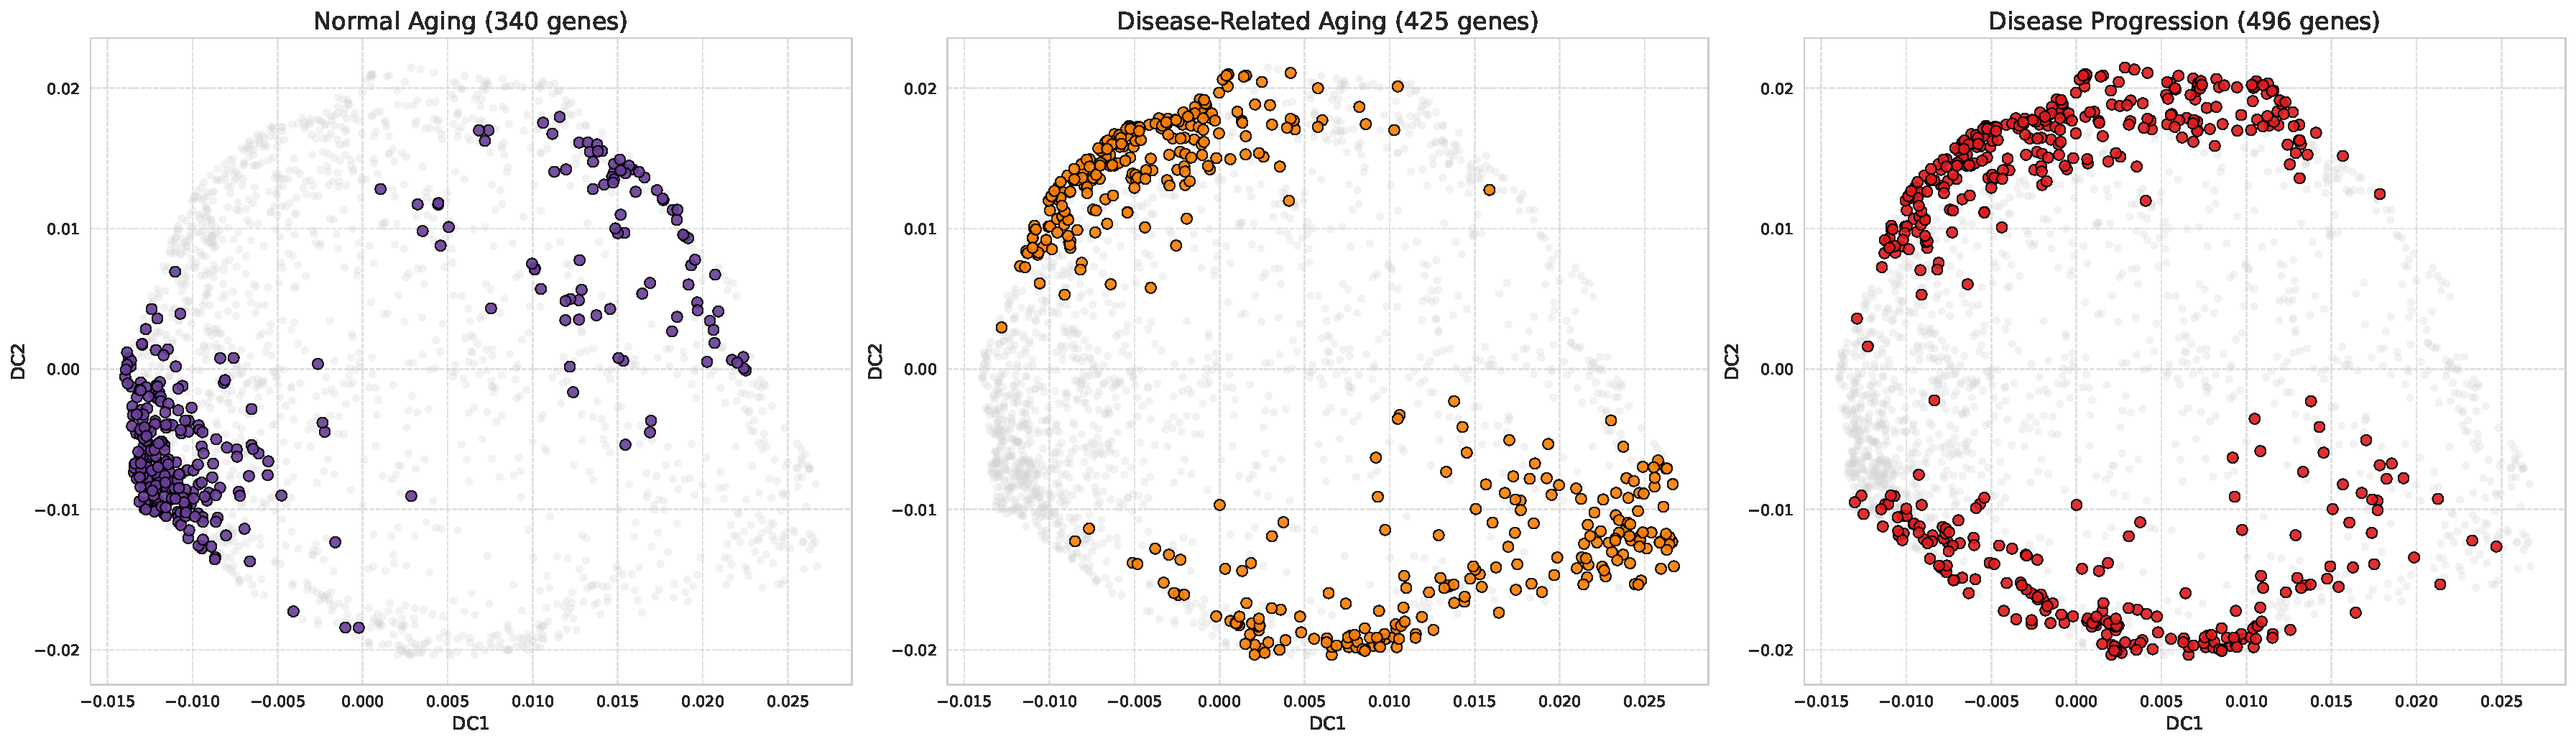
\includegraphics[width=\linewidth]{figures/kais_untreated-multi_panel_gene_sets.pdf}
        \caption{Kais - Untreated Only}
    \end{subfigure}
    \caption{Multi-panel visualization of gene sets for the analyses including only untreated samples.}
    \label{fig:multipanel_untreated_samples}
\end{figure}


\section*{My Figure}

Here is the figure we generated showing the composition of gene variance. 
See Figure~\ref{fig:gene_variance_hist}.

\begin{figure}[htbp]
    \centering % This centers the image
    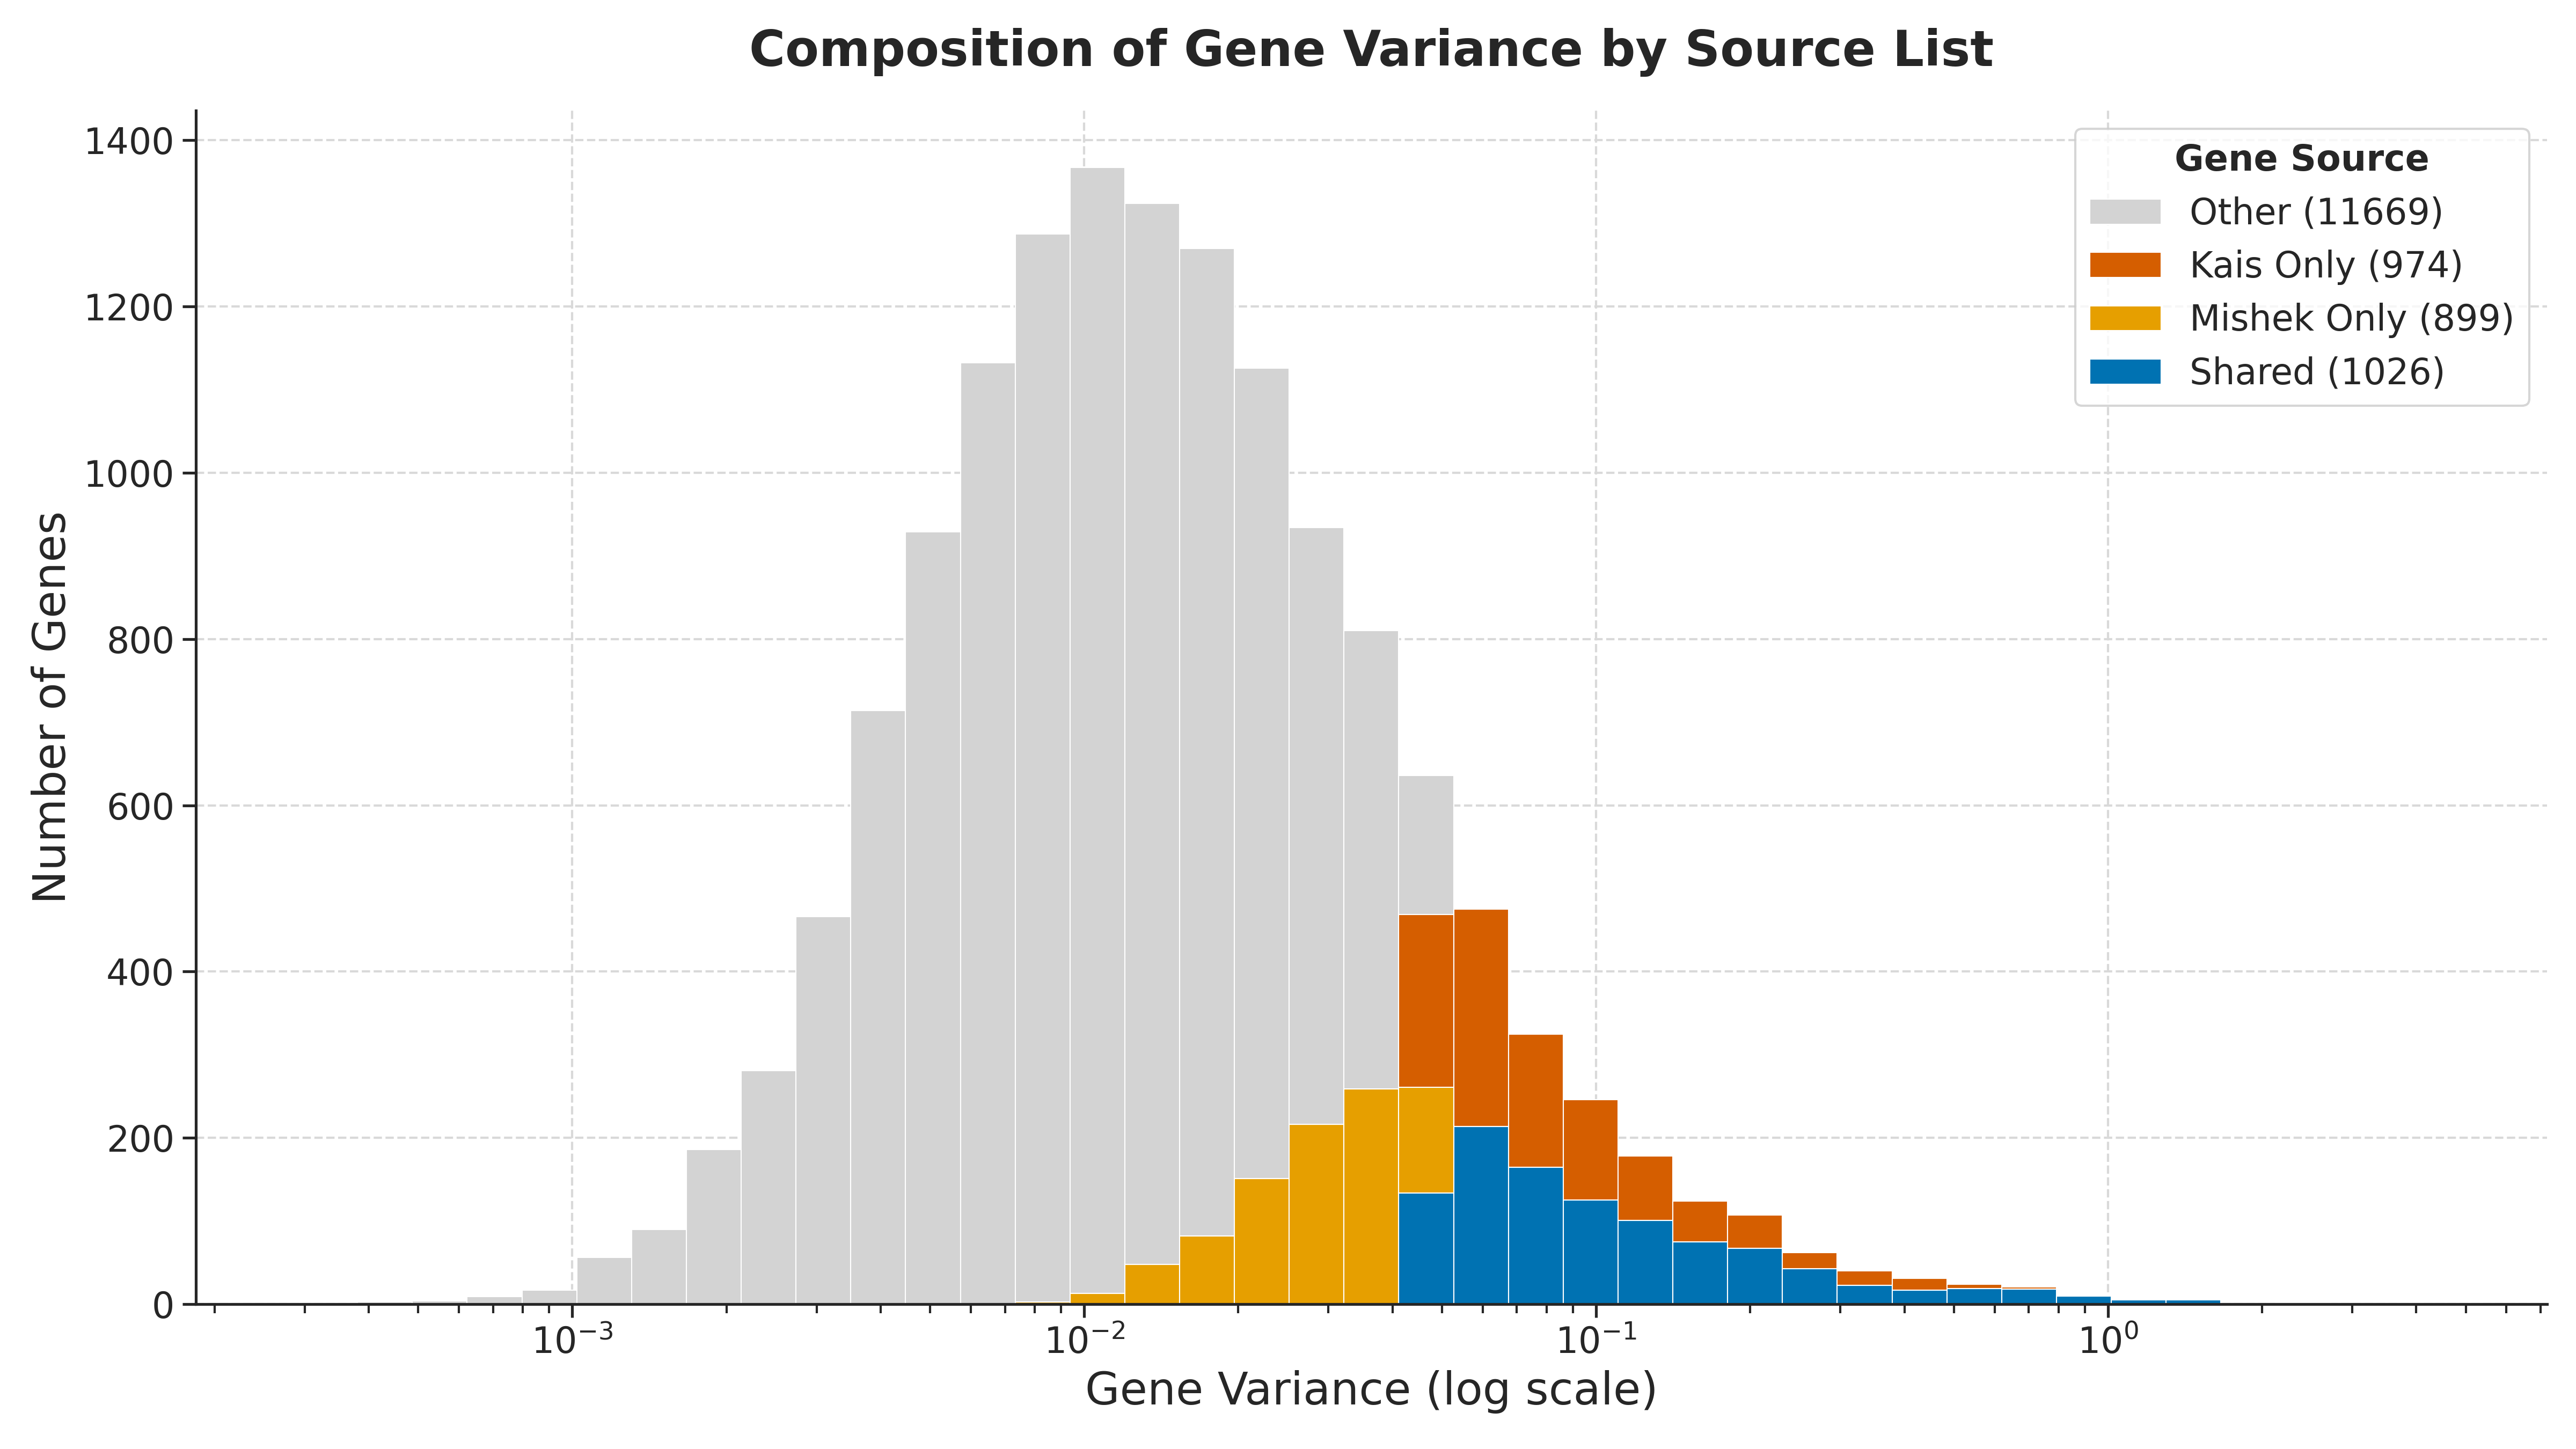
\includegraphics[width=0.9\textwidth]{figures/gene_variance_histogram_stacked_final.png}
    \caption{Composition of Gene Variance by Source List. The histogram shows the distribution of gene variances on a log scale, categorized by whether the genes were identified by the 'Kais' method, the 'Mishek' method, both (Shared), or neither (Other).}
    \label{fig:gene_variance_hist}
\end{figure}

\begin{figure}[htbp]
    \centering
    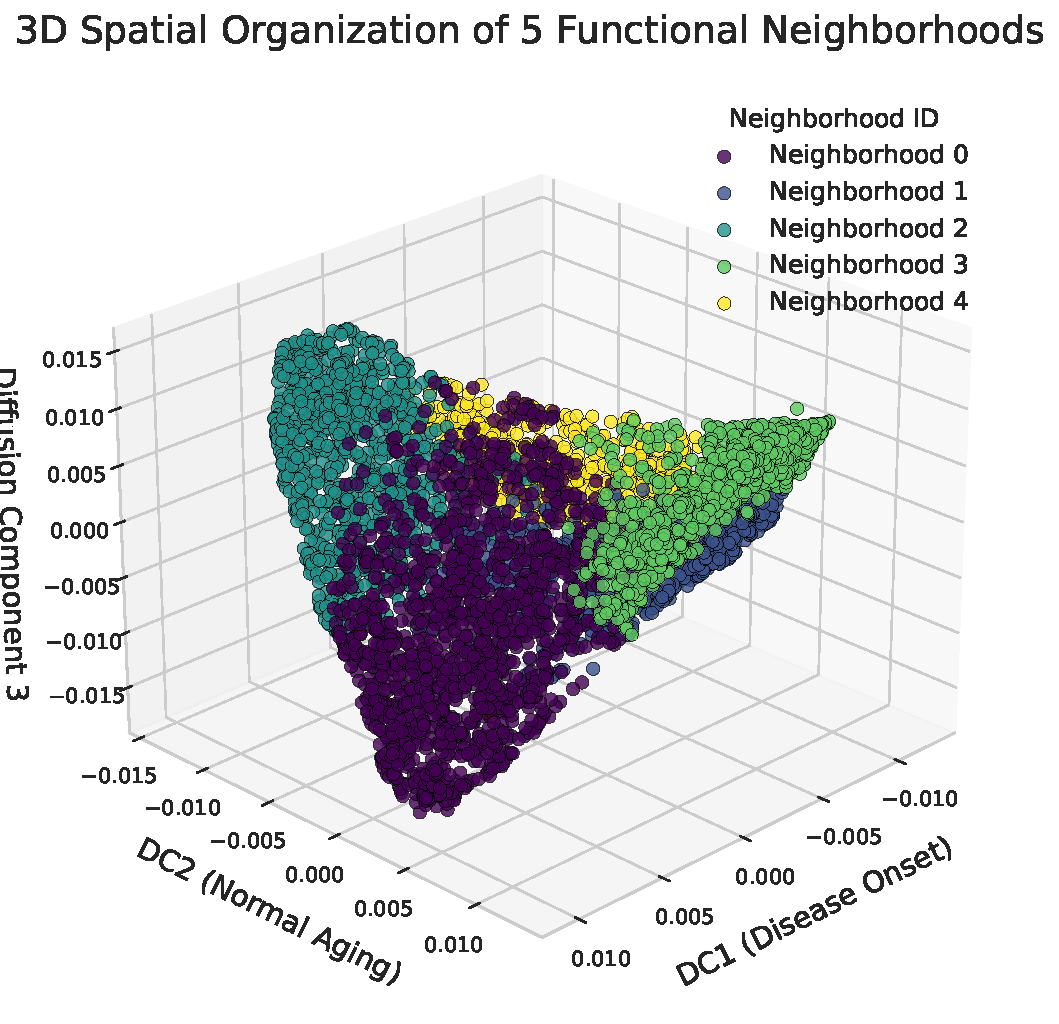
\includegraphics[width=0.65\textwidth]{figures/Fig_3B_Static_3D_Neighborhoods.pdf}
    \caption{\textbf{Static 3D Organization of Gene Neighborhoods}. The manifold is partitioned into 5 functional neighborhoods (Neighborhood 0 through 4) using K-means clustering.}
    \label{fig:static_neighborhoods}
\end{figure}

\begin{figure}[htbp]
    \centering
    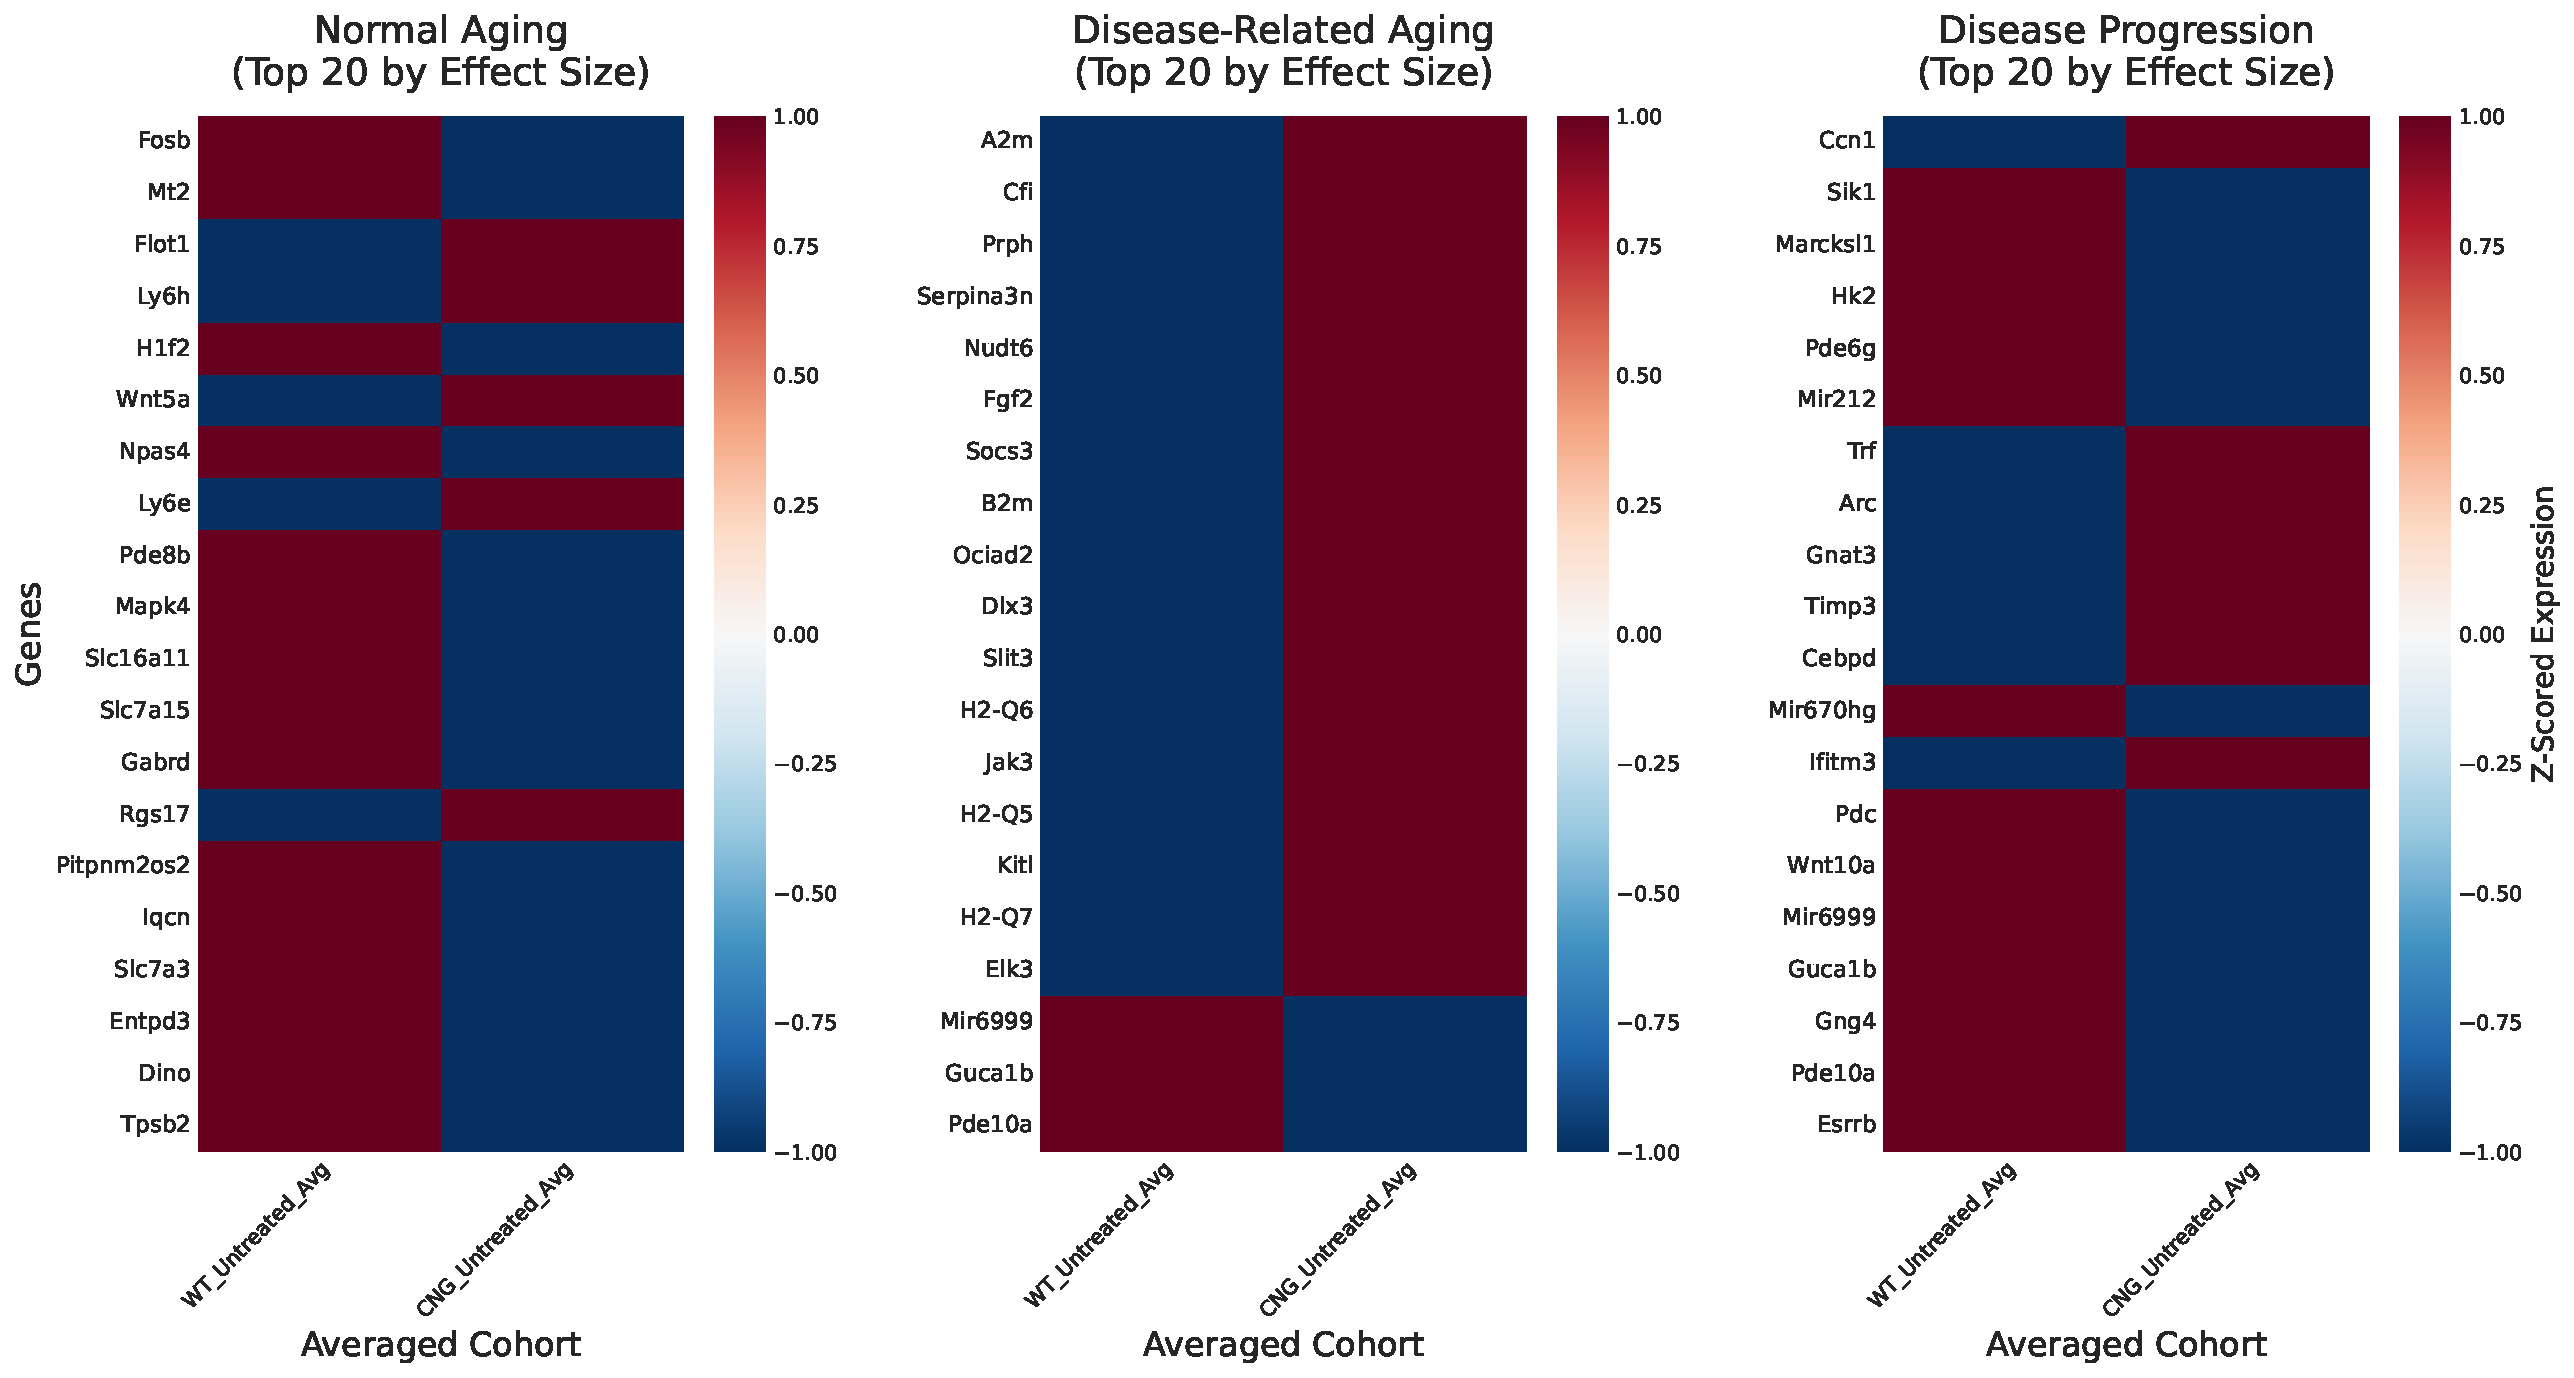
\includegraphics[width=0.5\textwidth]{figures/Figure_3_Top_Down_Heatmaps_by_Effect_Size.pdf}
    \caption{\textbf{Differential Gene Sets Reveal Distinct Processes}. Differential Gene Sets Reveal Distinct Transcriptional Processes. Heatmaps of the top 20 genes (ranked by effect size) highlight three biologically distinct gene sets. The definition of each set is based on comparisons from the multi-factorial DESeq2 model: \textbf{(Left) Normal Aging genes} are defined as those significantly changed in 7M WT vs. 1M WT retinas but *not* significantly changed in the late-stage disease comparison (CNG 7M vs. WT 1M). \textbf{(Center) Disease-Related Aging genes} are those significantly changed in late-stage disease (CNG 7M vs. WT 1M) but *not* significantly changed by normal aging (WT 7M vs. WT 1M). \textbf{(Right) Disease Progression genes} are defined as those significantly changed in late-stage disease (CNG 7M vs. WT 1M) but *not* significantly changed in early disease (CNG 1M vs. WT 1M).}
    \label{fig:aging_disease_heatmaps}
\end{figure}

\begin{figure}[htbp]
    \centering
    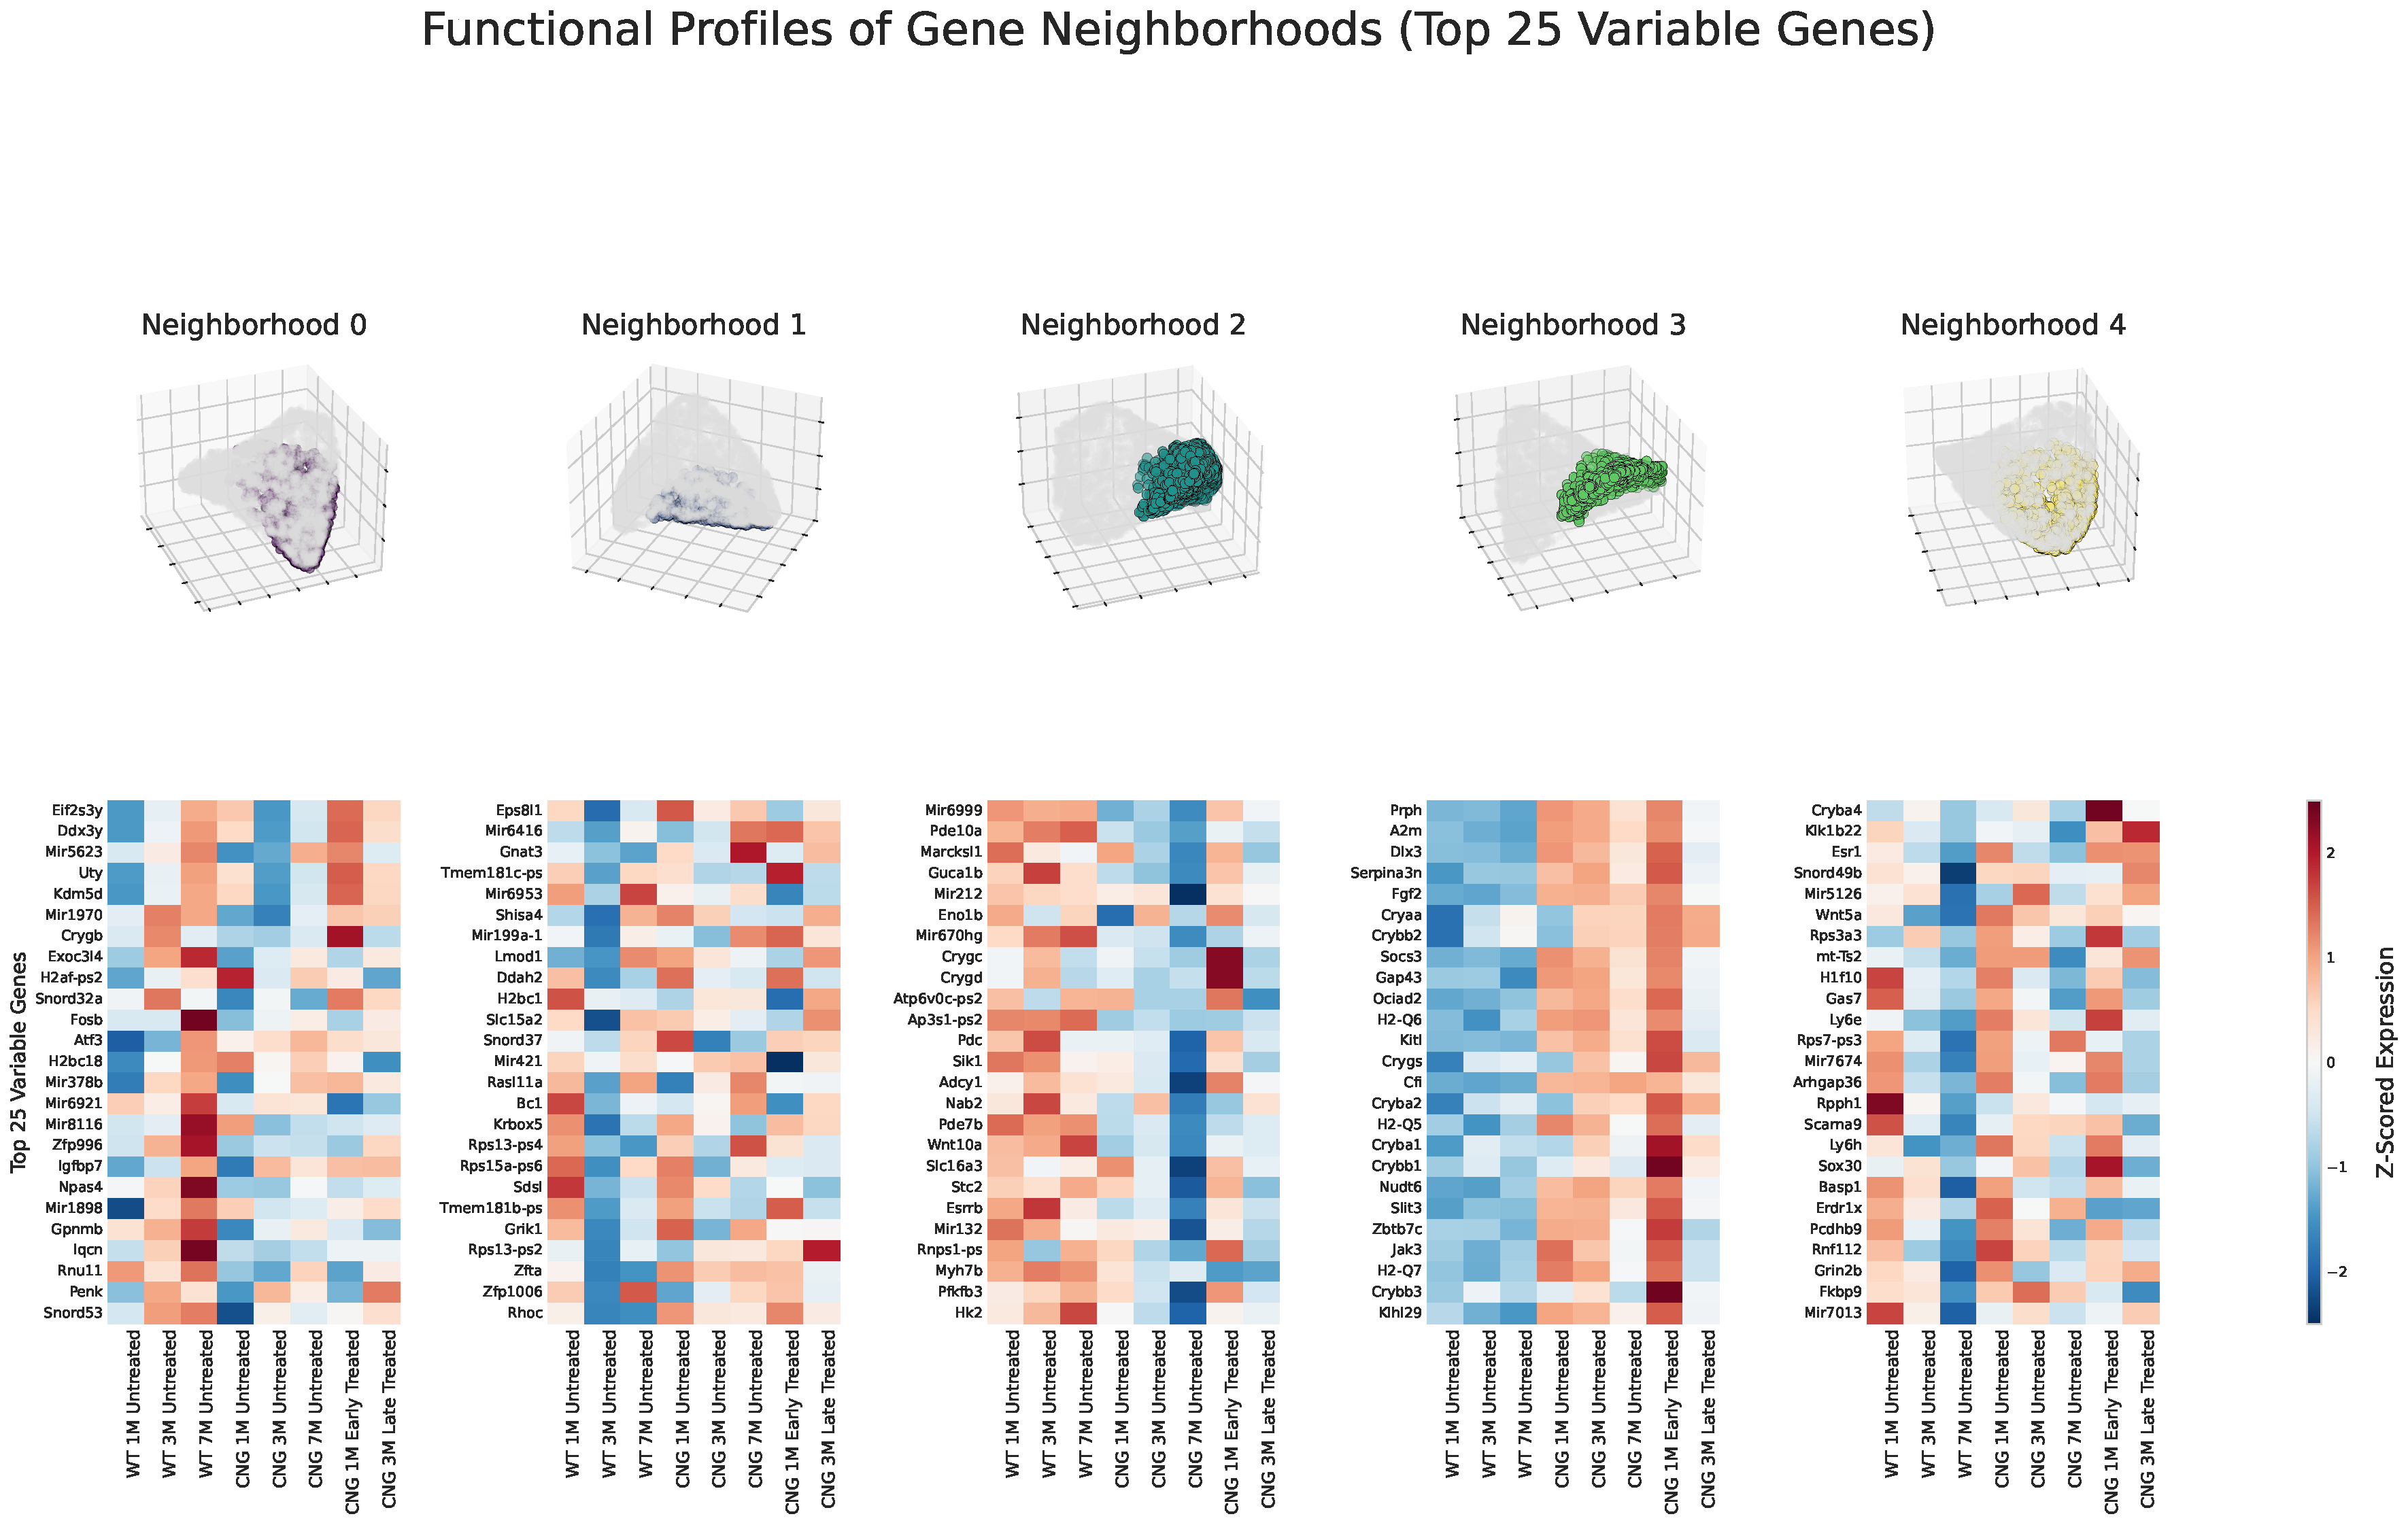
\includegraphics[width=\textwidth]{figures/Figure_4_Unbiased_Neighborhood_Profiles_All_Cohorts_FIXED.pdf}
    \caption{\textbf{Composite Profiles of Gene Neighborhoods}. Z-scored expression profiles of the top 25 most variable genes in each neighborhood across all 8 experimental cohorts.}
    \label{fig:neighborhood_profiles_heatmap}
\end{figure}

\begin{figure}[htbp]
    \centering
    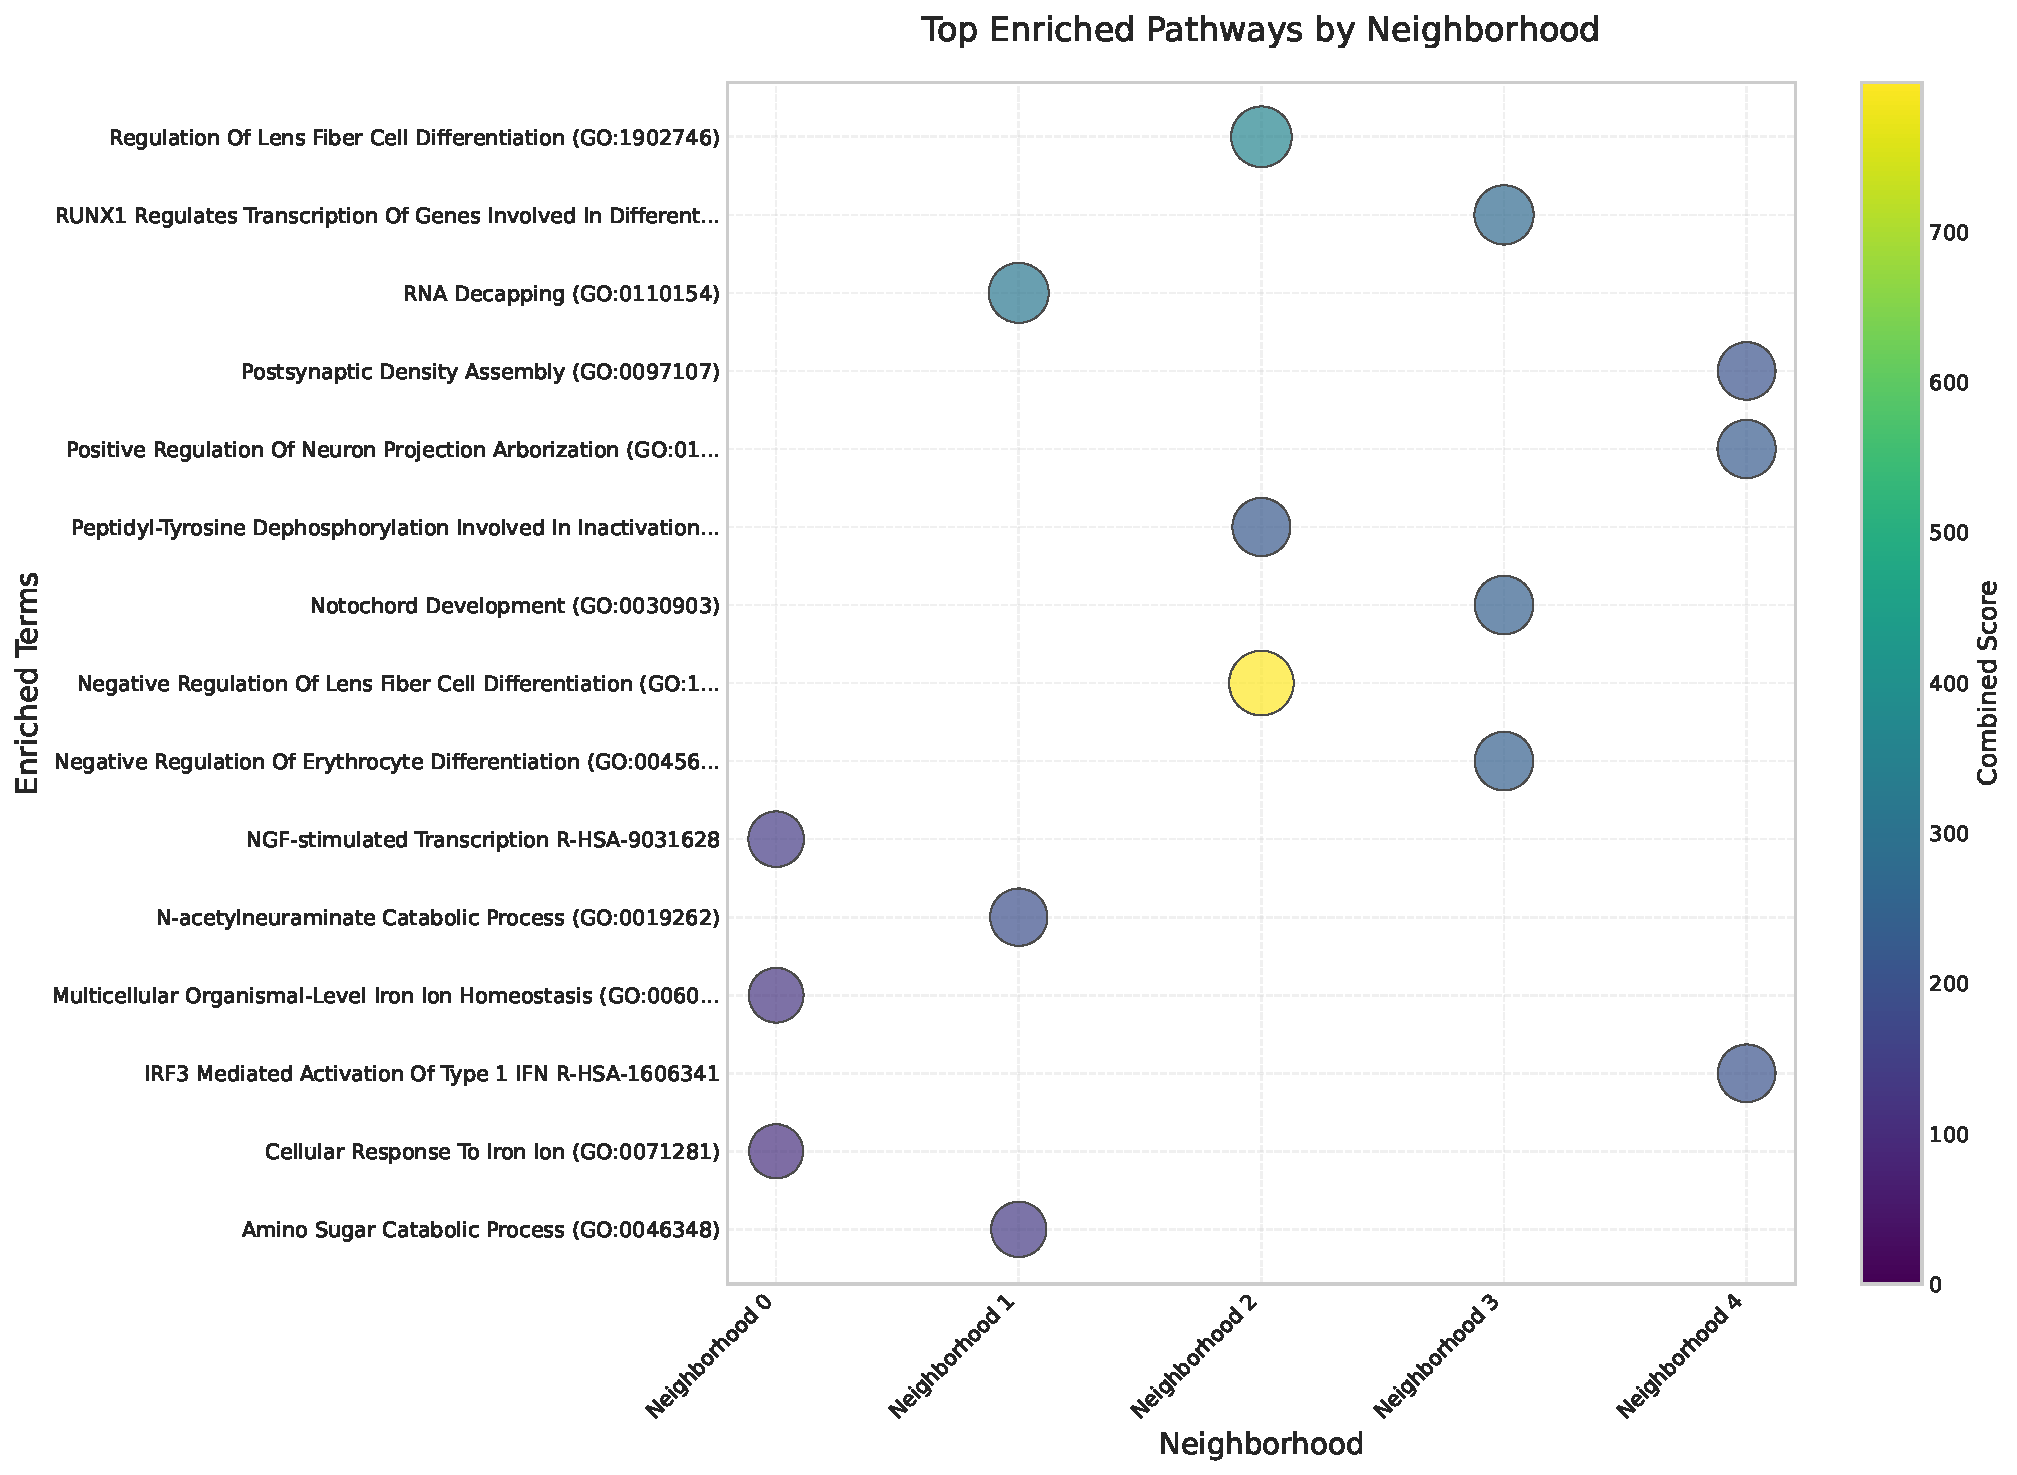
\includegraphics[width=0.8\textwidth]{figures/Figure_4A_GSEA_DotPlot.pdf}
    \caption{\textbf{Top Enriched Biological Pathways by Neighborhood}. GSEA validates the functional identity of each neighborhood, linking expression trajectories to known biological processes.}
    \label{fig:gsea_dot_plot}
\end{figure}

\begin{figure}[htbp]
    \centering
    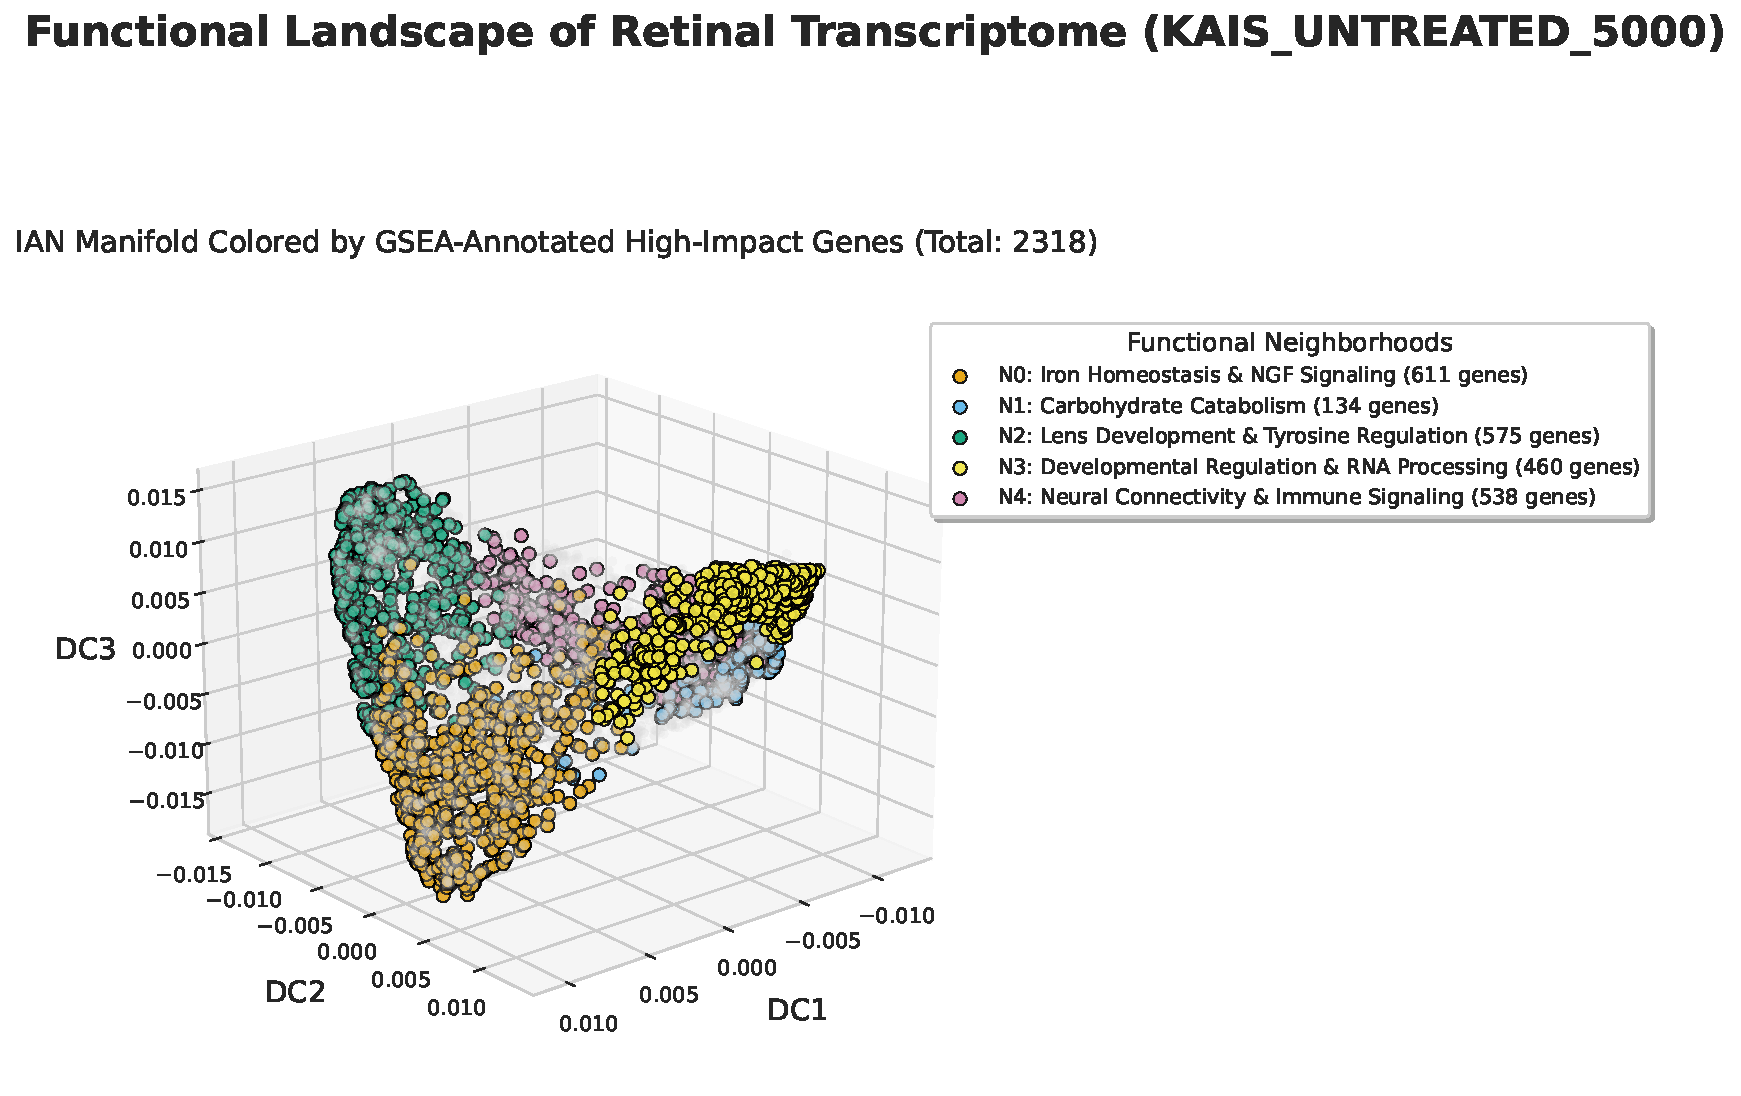
\includegraphics[width=0.8\textwidth]{figures/functional_lanscape.pdf}
    \caption{\textbf{Functional Landscape of the Retinal Transcriptome}. The IAN manifold is colored based on its 5 functional neighborhoods, with annotations derived from Gene Set Enrichment Analysis (GSEA). This figure highlights the spatial organization of high-impact genes according to the primary biological axes (DC1 and DC2) and DC3.}
    \label{fig:functional_landscape_3d}
\end{figure}


\bibliography{bibfile}


\end{document}
